\documentclass[a4paper,10pt]{book}
\usepackage[centertags]{amsmath}
\usepackage{amscd}
\usepackage{amsthm}
\usepackage{amssymb}
\usepackage{enumerate}
\usepackage{multicol}
\usepackage[english,catalan,spanish]{babel}
\usepackage[all]{xy}
\usepackage{color}
\usepackage{tikz}
\usepackage{indentfirst}
\usepackage[utf8]{inputenc}
\usepackage[T1]{fontenc}
\linespread{1.1}
\setlength{\parskip}{10pt}
\usepackage[twoside,bindingoffset=1cm]{geometry}
\usepackage{lmodern}
\usepackage[x11names, dvipsnames, table]{xcolor}
\definecolor{ubblue}{HTML}{0059A2}
\usepackage[colorlinks=true, linkcolor=black, citecolor=ubblue, urlcolor=ubblue]{hyperref}
\usepackage{cleveref}
\usepackage[protrusion=true,expansion=true]{microtype}
\usepackage{cite}
\usepackage{booktabs}
\usepackage{IEEEtrantools}
\usepackage{subcaption}
\usepackage{enumitem}
\setlist[itemize]{itemsep=4pt, parsep=2pt, topsep=2pt, leftmargin=*}
\setlist[enumerate]{itemsep=4pt, parsep=2pt, topsep=2pt, leftmargin=*}
\usepackage{chronology}
\usepackage{longtable}
\usepackage{dirtree}
\usepackage{tabularx}
\usepackage{caption}
\captionsetup[table]{labelfont=bf}

%% Custom packages


%%%%%%%%%%%%%%%%%%%%%%%%%%%%%%%%%%%%%%%%%%%%%%%%%%%%%%%%%%%%%%%%%%%%%%%%%%%
%%%% local definitions for this paper
%%%%%%%%%%%%%%%%%%%%%%%%%%%%%%%%%%%%%%%%%%%%%%%%%%%%%%%%%%%%%%%%%%%%%%%%%%%


%%%%%%%%%%%%%%%%%%%%%% aix{\`o} pels headings %%%%%%%%%%%%%%%%%%%%%%%%
\usepackage{fancyhdr}
\pagestyle{fancy}
\renewcommand{\chaptermark}[1]{\markboth{#1}{}}
\renewcommand{\sectionmark}[1]{\markright{\thesection\ #1}}
\fancyhf{} \fancyhead[LE,RO]{\bfseries\thepage}
\fancyhead[LO]{\bfseries\rightmark} \fancyhead[RE]{\bfseries\leftmark}

\def\paginaenblanc{\newpage%
\thispagestyle{empty}%
\vspace*{2cm}%
\newpage%
\thispagestyle{empty}%
}


%%%%%%%%%%%%%%%%%%%%%%%%%%%%%%%%%%%%%%%%%%%%%%%%%%%%%%%%%%%%%%%%%%%%%%%%%
% aux commands
%%%%%%%%%%%%%%%%%%%%%%%%%%%%%%%%%%%%%%%%%%%%%%%%%%%%%%%%%%%%%%%%%%%%%%%%%
%==========================================================================
% macros to support private authors' notes
%==========================================================================
\newif\ifprivate
\privatetrue
\def\xbar{\vskip0.09in\hrule\vskip0.06in}
\def\private#1{\ifprivate \xbar {\em #1} \xbar
\else \fi}
\def\huh{\ifprivate ??? \marginpar{\Huge ???}
\else \fi}
\def\???{\ifprivate {\bf {???}} \marginpar{\begin{center}{\Huge {\bf ?}}\end{center}}
\else \fi}
%\def\???{\ifprivate {\bf {???}} \marginpar{{\Huge {\bf ?}}}
%\else \fi}
\marginparsep1mm
\def\nota#1{\ifprivate  $\clubsuit$ \marginpar{\parbox[t]{2.4cm}{\begin{center}\tiny #1\end{center}}}
\else \fi}
\def\comment#1{\ifprivate \marginpar{\parbox[t]{2.4cm}{\begin{center}\tiny #1\end{center}}}
\else \fi}
%\def\nota#1{\ifprivate  $\clubsuit$ \marginpar{\parbox[t]{1.8cm}{\tiny #1}}
%\else \fi}
\def\privateeject{\ifprivate\eject\fi}
%\def\???{{\bf {???}} \marginpar{{\Huge {\bf ?}}} }
%%%%%%%%%%%%%%%%%%%%%%%%%%%%%%%%%%%%%%%%%%%%%%%%%%%%%%%%%%%%%%%%%%%%%%%%%%

%%%%%%%%%%%%%%%%%%%%%%%%%%%%%%%%%%%%%%%%%%%%%%%%%%%%%%%%%%%%%%%%%%%%%%%%
%%%%%%%%%%%%%%%%%%%%%%%%%%%%%%%%%%%%%%%%%%%%%%%%%%%%%%%%%%%%%%%%%%%%%%%%
\def\UrlBreaks{\do\/\do\-}
\begin{document}
\bstctlcite{IEEEexample:BSTcontrol}
\pagestyle{empty}

\begin{titlepage}
	\begin{center}
		\begin{figure}[htb]
			\begin{center}
				
\includegraphics[width=6cm]{assets/ub_color.pdf}
			\end{center}
		\end{figure}
				
		\def\worktitle{Evaluation of Transformer-Based Models for Molecular Subtype Classification of Invasive Ductal Breast Carcinoma Using Mammography}
				
		\textbf{\LARGE Treball final de grau} \\
		\vspace*{.5cm}
		\textbf{\LARGE GRAU D'ENGINYERIA INFORM\`{A}TICA } \\
		\vspace*{.5cm}
		\textbf{\LARGE Facultat de Matem\`atiques i Inform\`atica\\ Universitat de Barcelona} \\
		\vspace*{1.0cm}
		\rule{16cm}{0.1mm}\\
		\begin{Huge}
			\textbf{Evaluation of Transformer-Based Models for Molecular Subtype Classification of Invasive Ductal Breast Carcinoma Using Mammography} \\
		\end{Huge}
		\rule{16cm}{0.1mm}\\
				
		\vspace{1cm}
				
		\begin{flushright}
						
						
			\vspace*{2.5cm}
						
			\hfill
						
			\renewcommand{\arraystretch}{1.5}
			\begin{tabular}{ll}
				\textbf{\small Autor:}       & \textbf{\small David Bland\'on T\'orrez }                             \\
				\textbf{\small Director:}    & \textbf{\small Dr. Oliver D\'iaz Montesdeoca }                        \\
				\textbf{\small Realitzat a:} & \textbf{\small  Departament de Matem\`{a}tiques i  Inform\`{a}tica  } \\
				\textbf{\small Barcelona,}   & \textbf{\small \today }                                               
			\end{tabular}
						
		\end{flushright}
				
	\end{center}
		
\end{titlepage}

%%%%%%%%%%%%%%%%%%%%%%%%%%%%%%%%%%%%%%%%%%%%%%%%%%%%%%%%%%%%%%%%%%%%%%%%%
\newpage
\selectlanguage{english}
\noindent \textbf{\large Abstract}

Breast cancer remains the most prevalent malignancy and a leading cause of mortality in women worldwide. Early and accurate molecular characterization is critical for prognosis and treatment selection. Molecular subtyping, traditionally guided by invasive tissue biopsies and immunohistochemical analysis, enables personalized therapies but is costly, time-consuming, and not universally feasible. Non-invasive alternatives leveraging medical imaging, particularly mammography, have gained research interest for molecular classification.

This study evaluates the potential of Transformer-based DL models to classify molecular subtypes of invasive ductal carcinoma using mammographic images exclusively from the public CMMD (The Chinese Mammography Database)  dataset. A systematical analysis was conducted to compare three state-of-the-art Transformer architectures, Vision Transformer (ViT), Swin Transformer (Swin), and Multi-Axis Vision Transformer (MaxViT), against a traditional CNN model, ResNet-101. The experimental methodology addresses key challenges such as class imbalance through weighted loss functions, oversampling, data augmentation, and robust cross-validation strategies.

Results demonstrate that transformer-based models consistently outperform the CNN baseline. ViT achieved the highest average AUC (0.635 ± 0.016) and balanced accuracy (0.385 ± 0.042) on test sets, compared to ResNet-101 (AUC: 0.563 ± 0.03; balanced accuracy: 0.322 ± 0.062). Statistical analysis confirmed significant performance differences (p < 0.05), supporting the hypothesis that transformer self-attention mechanisms better model global spatial relationships in mammograms.

Despite these advances, overall performance remains below clinically acceptable thresholds, highlighting the inherent difficulty of non-invasive molecular subtyping based solely on imaging and the need for larger datasets or multimodal integration. Nevertheless, this work demonstrates the potential of transformer-based approaches for accessible, non-invasive breast cancer characterization, establishing a robust foundation for future AI-driven advancements in medical imaging.

%%%%%%%%%%%%%%%%%%%%%%%%%%%%%%%%%%%%%%%%%%%%%%%%%%%%%%%%%%%%%%%%%%%%%%%%%

%%%%%%%%%%%%%%%%%%%%%%%%%%%%%%%%%%%%%%%%%%%%%%%%%%%%%%%%%%%%%%%%%%%%%%%%%
\newpage
\selectlanguage{spanish}
\noindent \textbf{\large Resumen}

El cáncer de mama sigue siendo la neoplasia maligna más prevalente y una de las principales causas de mortalidad en mujeres a nivel mundial. La caracterización molecular temprana y precisa es crucial para el pronóstico y la selección de tratamientos. La subtipificación molecular, tradicionalmente basada en biopsias tisulares invasivas y análisis inmunohistoquímicos, permite terapias personalizadas, pero resulta costosa, consume tiempo y no siempre es viable. Las alternativas no invasivas que aprovechan imágenes médicas, particularmente la mamografía, han ganado interés investigativo para la clasificación molecular.

Este estudio evalúa el potencial de modelos de aprendizaje profundo basados en Transformers para clasificar subtipos moleculares de carcinoma ductal invasivo utilizando exclusivamente imágenes mamográficas del conjunto de datos público CMMD (The Chinese Mammography Database). Comparamos sistemáticamente tres arquitecturas Transformer de vanguardia: Vision Transformer (ViT), Swin Transformer (Swin) y Multi-Axis Vision Transformer (MaxViT), frente a una red neuronal convolucional (CNN) tradicional, ResNet-101. La metodología experimental aborda desafíos clave como el desbalance de clases mediante funciones de pérdida ponderadas, sobremuestreo, aumentación de datos y estrategias robustas de validación cruzada.

Los resultados indican que los modelos basados en Transformers superan consistentemente a la CNN de referencia. ViT logró el mayor AUC promedio (0.635 ± 0.016) y precisión balanceada (0.385 ± 0.042) en los conjuntos de prueba, frente a ResNet-101 (AUC: 0.563 ± 0.03; precisión balanceada: 0.322 ± 0.062). El análisis estadístico confirma diferencias significativas (p < 0.05), respaldando la hipótesis de que los mecanismos de autoatención en Transformers modelan mejor las relaciones espaciales globales en mamografías.

A pesar de estos avances, el rendimiento general sigue estando por debajo de los umbrales clínicamente aceptables, subrayando la dificultad inherente de la subtipificación molecular no invasiva basada únicamente en imágenes y la necesidad de investigar con conjuntos de datos más amplios o integración multimodal. No obstante, este trabajo demuestra el potencial de los enfoques basados en Transformers para caracterizar el cáncer de mama de manera accesible y no invasiva, estableciendo un referente sólido para futuros avances en imágenes médicas impulsadas por IA.

%%%%%%%%%%%%%%%%%%%%%%%%%%%%%%%%%%%%%%%%%%%%%%%%%%%%%%%%%%%%%%%%%%%%%%%%%

%%%%%%%%%%%%%%%%%%%%%%%%%%%%%%%%%%%%%%%%%%%%%%%%%%%%%%%%%%%%%%%%%%%%%%%%%
\newpage
\selectlanguage{catalan}
\noindent \textbf{\large Resum}

El càncer de mama continua sent la neoplàsia maligna més prevalent i una de les principals causes de mortalitat en dones a nivell mundial. La caracterització molecular precoç i precisa és crucial per al pronòstic i la selecció de tractaments. La subtipificació molecular, tradicionalment basada en biòpsies tissulars invasives i anàlisi immunoistoquímics, permet teràpies personalitzades, però resulta costosa, consumeix temps i no sempre és viable. Les alternatives no invasives que aprofiten imatges mèdiques, particularment la mamografia, han guanyat interès investigador per a la classificació molecular.

Aquest estudi avalua el potencial de models d'aprenentatge profund (DL) basats en Transformers per classificar subtipus moleculars de carcinoma ductal invasiu utilitzant exclusivament imatges mamogràfiques del conjunt de dades públic CMMD. Comparem sistemàticament tres arquitectures Transformer d'avantguarda: Vision Transformer (ViT), Swin Transformer (Swin) i Multi-Axis Vision Transformer (MaxViT), front a una xarxa neuronal convolucional (CNN) tradicional, ResNet-101. La metodologia experimental aborda reptes clau com el desequilibri de classes mitjançant funcions de pèrdua ponderades, sobremostreig, augmentació de dades i estratègies robustes de validació creuada.

Els resultats indiquen que els models basats en Transformers superen consistentment la CNN de referència. ViT va assolir el major AUC mitjà (0,635 ± 0,016) i precisió balancejada (0,385 ± 0,042) en els conjunts de prova, front a ResNet-101 (AUC: 0,563 ± 0,03; precisió balancejada: 0,322 ± 0,062). L'anàlisi estadística confirma diferències significatives (p < 0,05), recolzant la hipòtesi que els mecanismes d'autoatenció en Transformers modelen millor les relacions espacials globals en mamografies.

Malgrat aquests avenços, el rendiment global segueix estant per sota dels llindars clínicament acceptables, subratllant la dificultat inherent de la subtipificació molecular no invasiva basada únicament en imatges i la necessitat d'investigar amb conjunts de dades més amplis o integració multimodal. No obstant això, aquest treball demostra el potencial dels enfocaments basats en Transformers per caracteritzar el càncer de mama de manera accessible i no invasiva, establint un referent sòlid per a futurs avenços en imatges mèdiques impulsades per IA.

%%%%%%%%%%%%%%%%%%%%%%%%%%%%%%%%%%%%%%%%%%%%%%%%%%%%%%%%%%%%%%%%%%%%%%%%%
\newpage
\selectlanguage{english}
\noindent \textbf{\large Acknowledgements}

First and foremost, I wish to express my deepest gratitude to Dr. Oliver Díaz Montesdeoca for his guidance, patience, and unwavering support throughout this process. His valuable advice and mentorship have been fundamental to the completion of this work.

I dedicate this achievement to my family, to those who are with us and to those who are no longer here, especially my parents and siblings. Thank you for your unconditional love, for believing in me, and for always being my greatest inspiration; without you, I would not be the person I am today.

I also extend my gratitude to my second family, Martha and Adriana, for their constant encouragement and for taking care of me at every stage of this journey.

I am equally grateful to my friends Jose, Sergio, Teo, and Jordi, for making university a more enjoyable place and for their incomparable companionship.

And above all, thank you to Mabel, for being the energy and the light of my life. \textit{Todo esto es por ti}.
%%%%%%%%%%%%%%%%%%%%%%%%%%%%%%%%%%%%%%%%%%%%%%%%%%%%%%%%%%%%%%%%%%%%%%%%%
\selectlanguage{english}
\pagenumbering{roman} \setcounter{page}{0}
\let\cleardoublepage\clearpage
\tableofcontents
\newpage \thispagestyle{empty}
%%%%%%%%%%%%%%%%%%%%%%%%%%%%%%%%%%%%%%%%%%%%%%%%%%%%%%%%%%%%%%%%%%%%%%%%%

\listoffigures
\listoftables


\pagestyle{fancy}
\markboth{Introducción}{Introducción}
\newpage \thispagestyle{empty}
%%%%%%%%%%%%%%%%%%%%%%%%%%%%%%%%%%%%%%%%%%%%%%%%%%%%%%%%%%%%%%%%%%%%%%%%%
\mainmatter
\chapter{Introduction}
\section{Problem Context}

Breast cancer is one of the leading causes of mortality among women and the most common cancer type in this population. It is estimated that, on average, one in every twenty women worldwide will be diagnosed with breast cancer during their lifetime \cite{kim_global_2025}. Recent projections suggest that, if the current trend continues, by 2050 there will be approximately 3.2 million new cases and 1.1 million deaths from this disease, with a particularly significant impact in countries with low Human Development Index (HDI) scores \cite{kim_global_2025}.

In this context, early diagnosis and diagnostic imaging tools play a fundamental role in improving patient prognosis and survival \cite{wang_early_2017}. However, breast cancer is a heterogeneous disease\footnote{Cellular diversity present within a tumor (intratumoral heterogeneity) or between different tumors in the same individual (intertumoral heterogeneity).} that can be classified into various subtypes according to clinical and, particularly, molecular characteristics. The 2013 St. Gallen International Consensus Guidelines \cite{goldhirsch_personalizing_2013} defined four main subtypes based on hormone receptors (estrogen and progesterone) and the proliferation marker Ki67: Luminal A, Luminal B, HER2 positive (HER2-enriched), and Triple Negative (see Figure \ref{fig:subtypes}). This classification has direct clinical implications, as prognosis, therapeutic response, and treatment options are largely determined by the molecular subtype of the tumor.

Currently, molecular tumor characterization is mainly performed through tissue biopsy, an invasive and costly procedure that may require repetition, potentially delaying treatment initiation and increasing the clinical, physical, and emotional burden on patients. Therefore, there is a growing need to develop non-invasive, accessible, and efficient methods for reliable molecular subtype classification. In this regard, x-ray mammography stands out as the gold standard imaging modality, as it is a non-invasive, low-cost technique widely utilized for breast cancer screening and diagnosis due to its demonstrated effectiveness in clinical practice.

\begin{figure}
	\centering
	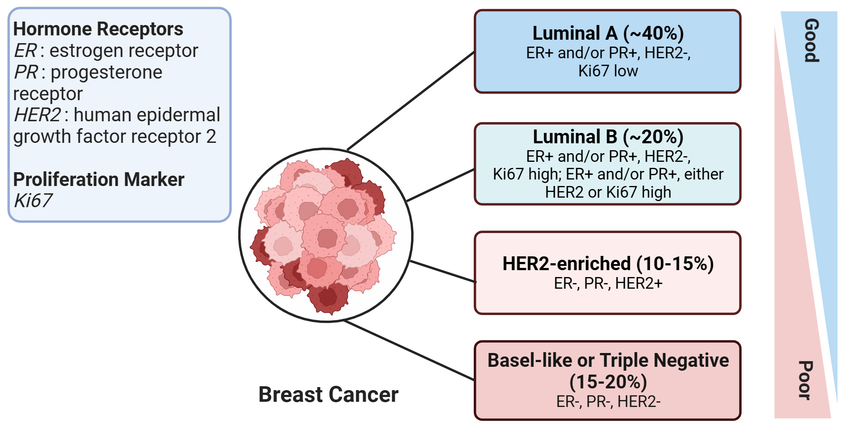
\includegraphics[width=0.8\linewidth]{reports/assets/subtypes.png}
	\caption[Classification of breast cancer molecular subtypes.]{Classification of breast cancer molecular subtypes, showing approximate proportions (\%) among all breast cancer cases. Subtypes are ordered by prognosis severity, with those having better outcomes at the top and progressively worse prognoses toward the bottom \cite{harnessing_2024}.}
	\label{fig:subtypes}
\end{figure}

In recent years, advances in artificial intelligence (AI), together with the increasing availability of data and increasingly powerful computational resources, have driven the development of deep learning (DL) models for breast cancer classification, detection, and prognosis prediction, as well as applications in other diseases. Several studies have demonstrated that these systems can match or even surpass the performance of human experts or CAD\footnote{Computer-Aided Diagnosis} systems in these tasks \cite{mckinney_international_2020,pattanaik_breast_2022,meenalochini_deep_2024,hussain_performance_2025}, highlighting the significant potential of this technology to improve clinical practice and patient outcomes.

Recent research has explored breast cancer molecular subtype classification from mammographic images. For example, Mota et al. (2024) \cite{mota_breast_2024} investigated this challenge, achieving a multi-class area under the curve (AUC)\footnote{A metric used in machine learning to evaluate the performance of classification models.} of 60.62\% using a ResNet-101 architecture. Similarly, Rabah et al. (2025) \cite{ben_rabah_multimodal_2025} obtained an AUC of 61.3\% with a Xception model in unimodal\footnote{Use only one type of data as input (images, text, video, etc.).} settings and developed a multimodal approach integrating clinical metadata, which achieved 88.87\% AUC. While unimodal approaches yield modest performance that remains below clinically acceptable thresholds (~80\% AUC), these studies highlight the diagnostic potential of mammographic imaging and underscore the importance of continued research to improve the accuracy and clinical utility of these models.

This study proposes a unimodal approach based exclusively on the inference based on mammograms from the public CMMD dataset (The Chinese Mammography Database) \cite{cai_online_2023}, comparing the performance of state-of-the-art Transformer architectures including Vision Transformer (ViT), Swin Transformer (Swin), and Multi-Axis Vision Transformer (MaxViT) against a traditional ResNet-101 baseline. While multimodal models typically achieve superior results by integrating complementary clinical data, a unimodal approach focused exclusively on mammographic images offers significant practical advantages, especially in resource-limited settings or when clinical data standardization is unavailable. Recent studies have demonstrated that Transformers-based models outperform convolutional neural networks (CNN) in accuracy and robustness for medical image classification tasks due to their self-attention mechanisms, which enable them to capture global spatial relationships across images \cite{mauricio_comparing_2023}. Based on these architectural advantages, this study hypothesizes that Transformer architectures will achieve superior performance in molecular subtype classification, even under a unimodal approach.

Ultimately, this work seeks to contribute to the development of non-invasive diagnostic tools through systematic evaluation of transformer-based models, advancing automated, accessible, and efficient molecular characterization of breast cancer. This approach is particularly valuable in clinical scenarios where tissue biopsy is not immediately feasible, potentially improving diagnostic equity and reducing time to treatment initiation.


\section{Planning}

\subsection{Objectives}

The \textbf{primary objective} of this study is to systematically compare Transformer-based architectures against a CNN baseline for mammography-based molecular subtype classification, establishing performance benchmarks for non-invasive breast cancer characterization.

To achieve this primary objective, the following \textbf{secondary objectives} are proposed:

\begin{enumerate}
	\item \textbf{Conduct a comprehensive literature review} of AI approaches for breast cancer molecular subtype classification, analyzing current research and performance benchmarks.
	\item \textbf{Identify and address dataset challenges} through appropriate preprocessing strategies, including class imbalance mitigation via weighted loss functions, balanced sampling techniques, and data augmentation methods.
	\item \textbf{Develop and implement} a robust stratified k-fold cross-validation framework for training and evaluating Vision Transformer architectures (ViT, Swin and MaxViT) on mammographic images.
	\item \textbf{Establish comparative performance analysis} against a ResNet-101 baseline and benchmark results from existing literature using standardized evaluation metrics (Accuracy, AUC, F1-Score, Precision, Recall, Cohen-Kappa).
	\item \textbf{Perform statistical validation} of model performance differences through statistical tests to ensure result significance and reliability.
        \item \textbf{Conduct a comparative analysis} with recent literature to identify advancements and the practical implications of the findings.
	\item \textbf{Apply interpretability analysis} using Grad-CAM and attention visualization techniques to identify mammographic features most relevant to molecular subtype discrimination.
	\item \textbf{Synthesize findings and provide recommendations} for future research directions and clinical implementation considerations.
\end{enumerate}

\subsection{Tasks to Develop}

In order to address the aforementioned objectives of the project, several tasks have been identified, as described below. 

\textbf{State of the Art}

\begin{enumerate}
	\item \textbf{Medical context}: Review current scientific literature on breast cancer to contextualize its clinical and epidemiological relevance.
	\item \textbf{Problem intuition}: Analyze the importance of molecular characterization in breast cancer, highlighting its advantages, limitations, and current challenges.
	\item \textbf{Previous works}: Examine recent advances in AI and DL for breast cancer characterization and diagnosis, comparing approaches and results reported in the literature.
\end{enumerate}

\textbf{Implementation}

\begin{enumerate}
	\item \textbf{Data Collection}: Acquire images and familiarize with the dataset's structure, organization, and provided metadata.
	\item \textbf{Data Analysis and Preprocessing}: Analyze class distribution, data consistency, and perform image preprocessing.
	\item \textbf{Project Coding}: Develop code to conduct experiments, train, and evaluate the different models.
	\item \textbf{Result Analysis}: Evaluate and interpret results to draw conclusions and propose future work.
\end{enumerate}

\textbf{Report Preparation}

\begin{enumerate}
	\item \textbf{Report Writing}: Document all procedures, including methodology, materials, results, and conclusions.
	\item \textbf{Revisions}: Incorporate feedback from advisor and refine until achieving acceptable quality.
	\item \textbf{Submission and Presentation}: Submit the thesis and prepare a summary of key findings for the committee presentation.
\end{enumerate}

\subsection{Planning}

The project planning is represented in the Gantt chart below (Figure \ref{fig:roadmap}), outlining previously defined tasks across the 4 months of the project (Spring Semester).

\begin{figure}[h!]
	\centering
	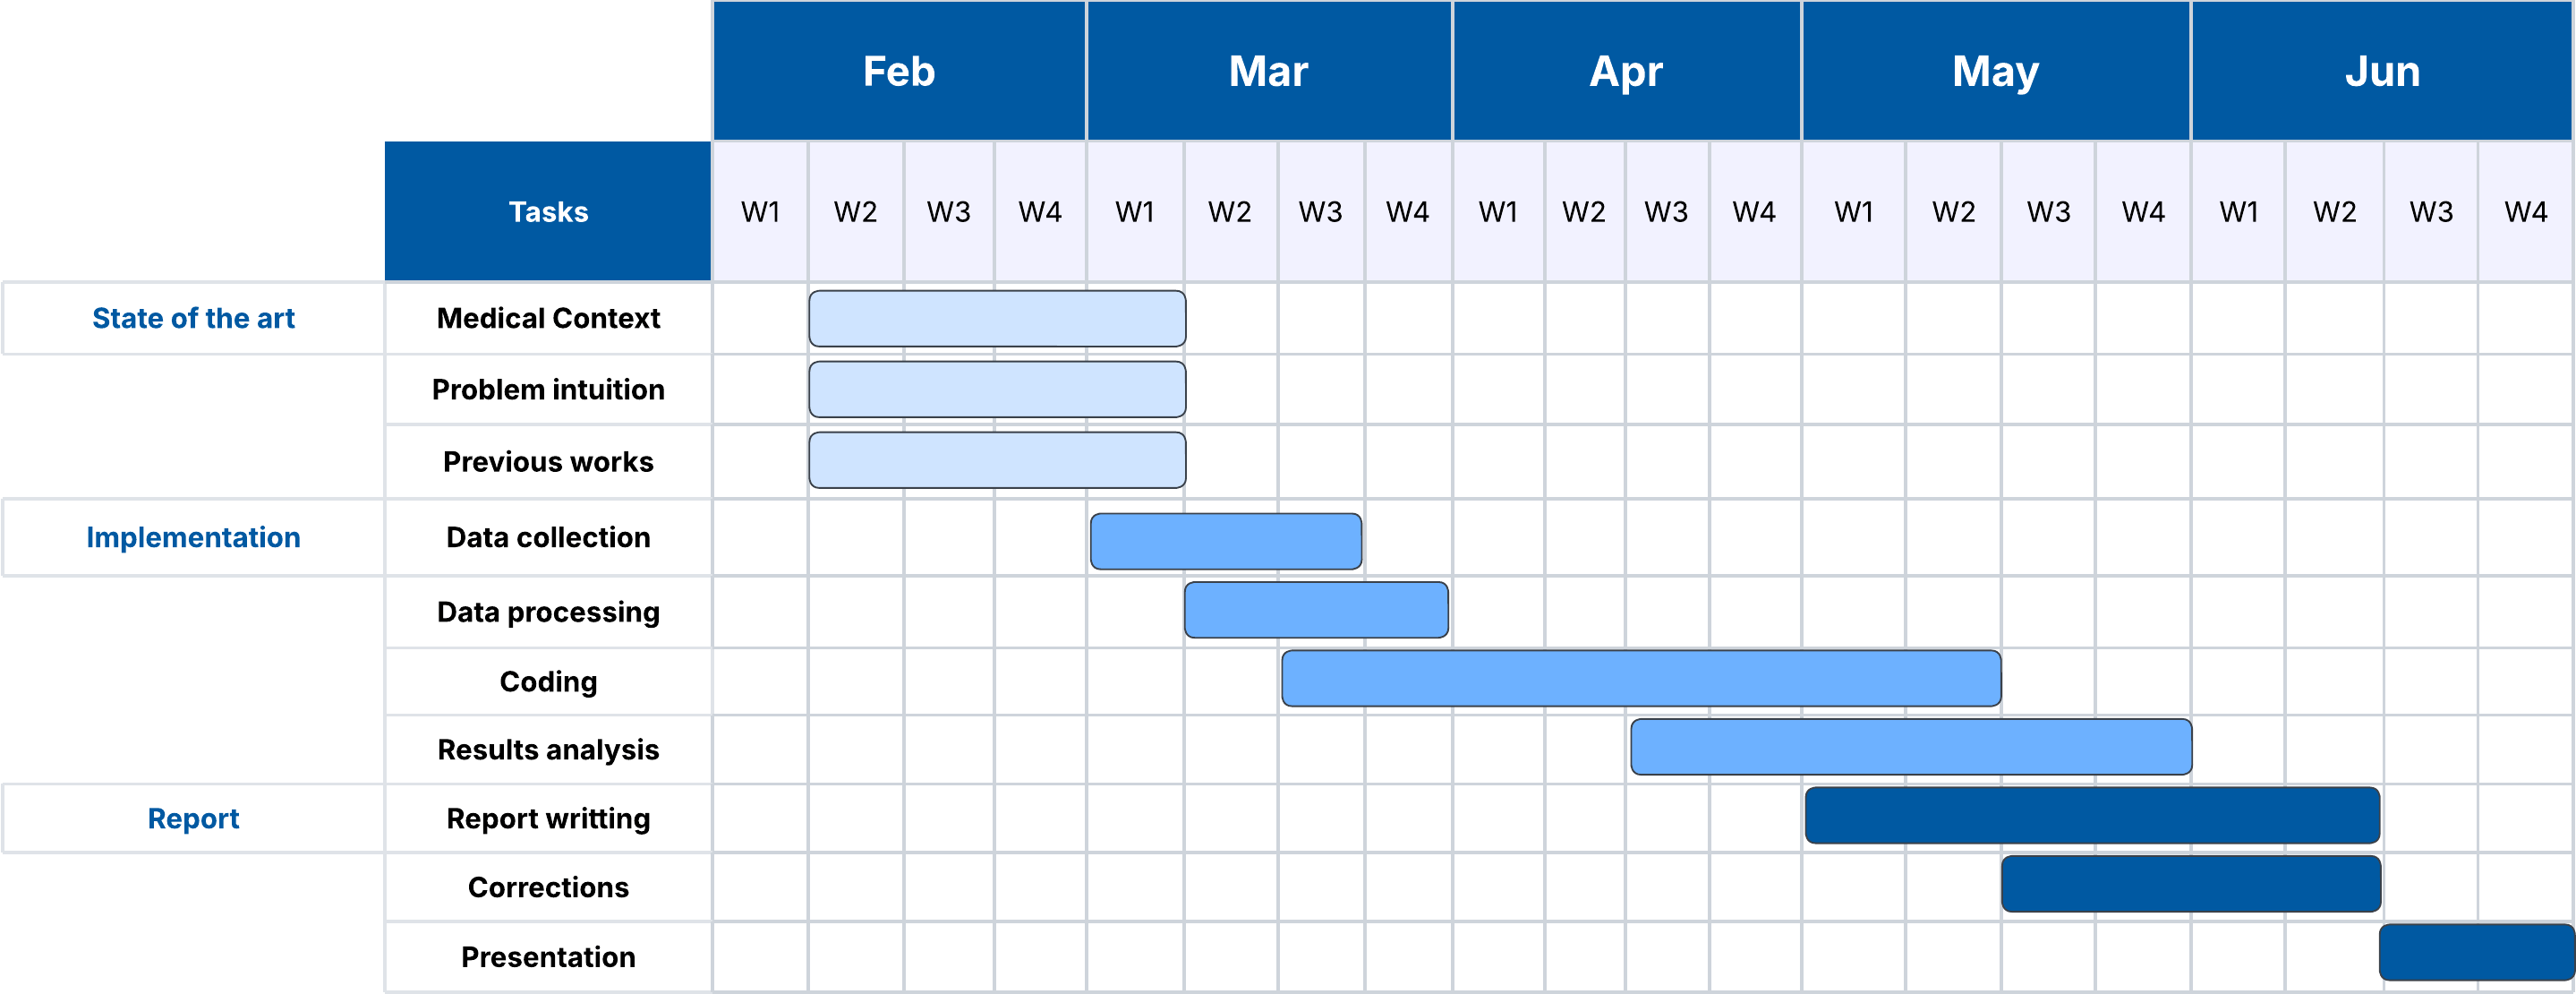
\includegraphics[width=1\linewidth]{reports//assets/RoadmapV3.png}
	\caption[Planning Gantt Chart]{Gantt Chart.}
	\label{fig:roadmap}
\end{figure}

%%%%%%%%%%%%%%%%%%%%%%%%%%%%%%%%%%%%%%%%%%%%%%%%%%%%%%%%%%%%%%%%%%%%%%%%%

\chapter{Background}

\section{Breast Cancer}

Breast cancer is a malignant neoplasm\footnote{An abnormal and uncontrolled growth of cells that gives rise to a mass or tumor, called benign if it grows slowly and remains localized, or malignant if it is invasive and fast-growing.} that originates in the glandular tissue of the breast, mainly in the ducts and lobules, where certain cells undergo genetic mutations that disrupt their growth control. 

These alterations allow cells to multiply uncontrollably, forming tumor masses that can infiltrate adjacent tissues and even spread to distant organs through the lymphatic system and bloodstream. In the absence of early diagnosis and timely treatment, this spread, also known as metastasis, can seriously compromise patient survival. Figure \ref{fig:breast-cancer-anatomy} illustrates the anatomical structure of the breast, showing how tumors develop within normal breast tissue.

\begin{figure}[h]
	\centering
	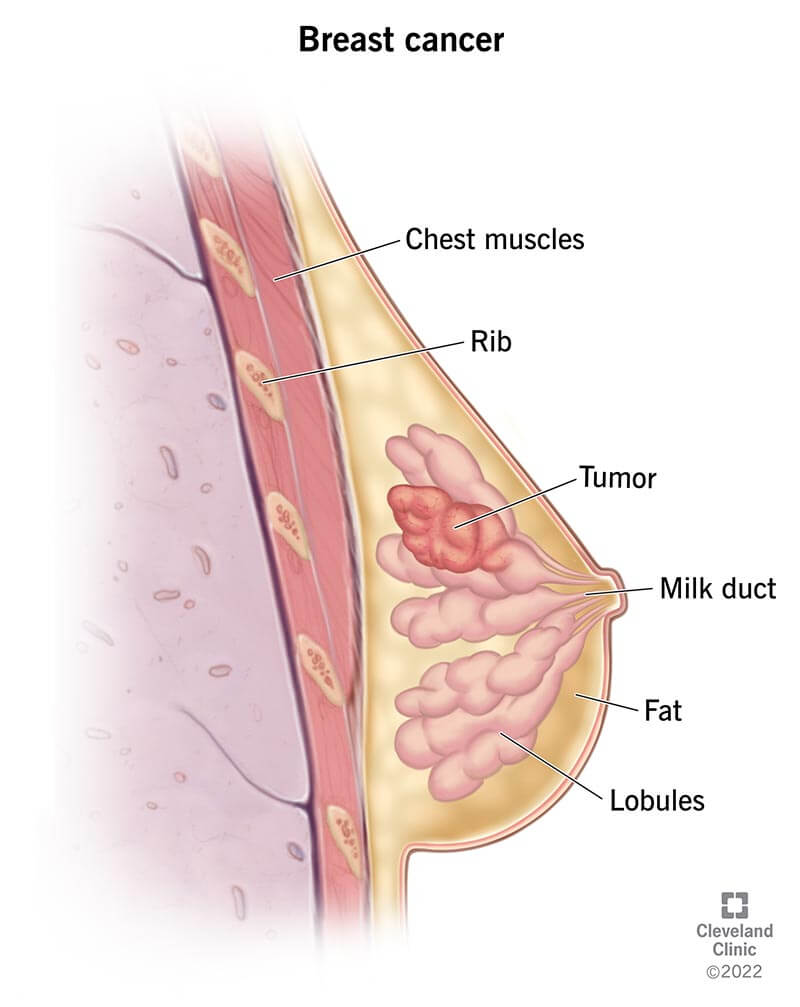
\includegraphics[width=0.3\linewidth]{reports//assets/bc.jpg}
	\caption[Anatomy of breast cancer]{Anatomy of breast cancer \cite{cleveland_clinic_breast_2023}.}
	\label{fig:breast-cancer-anatomy}
\end{figure}

\subsection{Epidemiology}

Globally, it is the most common neoplasm among women and the leading cause of cancer-related mortality in this population. In 2022, approximately 2.3 million new cases were estimated, with 670,000 deaths from this disease, according to the World Health Organization (WHO) \cite{who_breast_2024}. In Spain, breast cancer accounts for nearly 30\% of all cancer cases, and projections from the Spanish Society of Medical Oncology (SEOM) estimate around 37,400 new cases in 2025 \cite{seom_cancer_nodate}.

\subsection{Clinical Classification}

Most breast cancers are carcinomas, which are malignant tumors that originate in the ducts or lobules of the breast. These carcinomas constitute more than 95\% of all breast cancer cases \cite{makki_diversity_2015, noauthor_types_nodate}. From a clinical perspective, these tumors can be classified according to various criteria, among which the following stand out:

\textbf{According to their degree of invasion}
\begin{itemize}
	\item \textbf{Carcinoma in situ}: A tumor in which abnormal cells are confined within the breast ducts and have not crossed the natural barrier separating them from the rest of the breast tissue. Although not invasive, it is considered a precursor lesion and high-risk.
	\item \textbf{Invasive carcinoma}: A tumor that has breached the ducts or lobules of the breast and invaded the surrounding breast tissue. It can spread to lymph nodes or distant sites. 
\end{itemize}

\textbf{According to histological origin}
\begin{itemize}
	\item \textbf{Ductal carcinoma}: Originates in the milk ducts\footnote{Ducts that carry milk from the mammary glands to the nipple.} and is the most common subtype.
	\item \textbf{Lobular carcinoma}: Originates in the breast lobules and tends to show a more diffuse pattern of spread.
\end{itemize}

Figures \ref{fig:histological_types_one} and \ref{fig:histological_types_two} show the differences between ductal and lobular carcinoma, both in situ and invasive.

\begin{figure}[h!]
	\centering
	\begin{subfigure}[c]{0.48\textwidth}
		\centering
		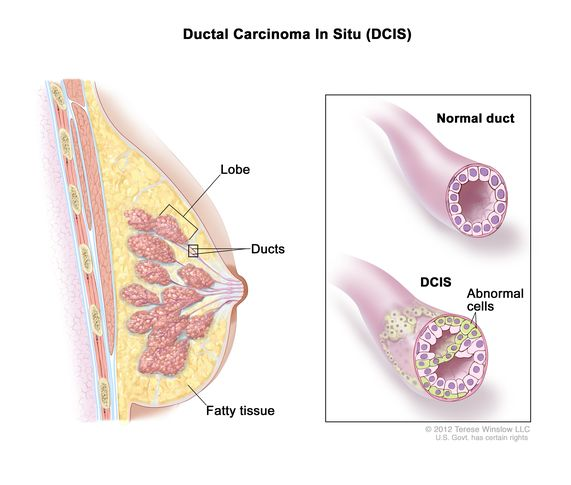
\includegraphics[width=\textwidth]{reports/assets/dcis.jpg}
		\caption{Ductal carcinoma in situ}
		\label{fig:dcis}
	\end{subfigure}
	\begin{subfigure}[c]{0.48\textwidth}
		\centering
		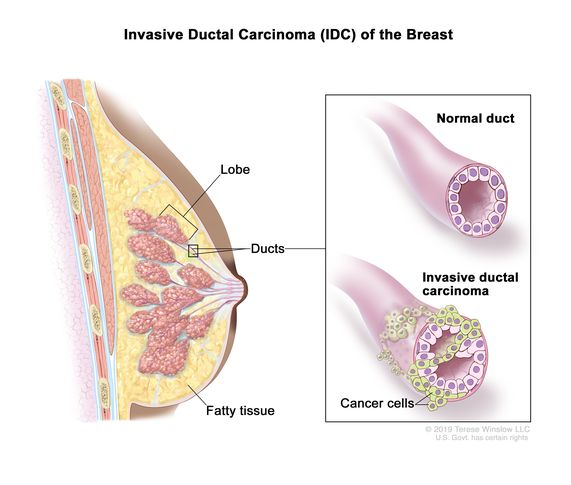
\includegraphics[width=\textwidth]{reports/assets/idc.jpg}
		\caption{Invasive ductal carcinoma}
		\label{fig:idc}
	\end{subfigure}
	\caption[DCIS vs. IDC comparison]{Anatomical comparison between ductal carcinoma in situ (DCIS) and invasive ductal carcinoma (IDC). (a) DCIS shows abnormal cells confined within the milk duct structure, while (b) IDC demonstrates cancer cells that have broken through the duct wall and invaded surrounding breast tissue \cite{noauthor_nci_2011}.}
	\label{fig:histological_types_one}
\end{figure}

\begin{figure}[h!]
	\centering
	\begin{subfigure}[c]{0.48\textwidth}
		\centering
		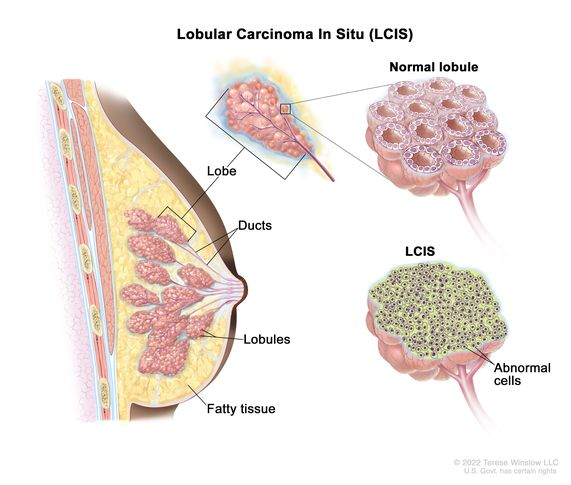
\includegraphics[width=\textwidth]{reports/assets/lcis.jpg}
		\caption{Lobular carcinoma in situ}
		\label{fig:lcis}
	\end{subfigure}
	\begin{subfigure}[c]{0.48\textwidth}
		\centering
		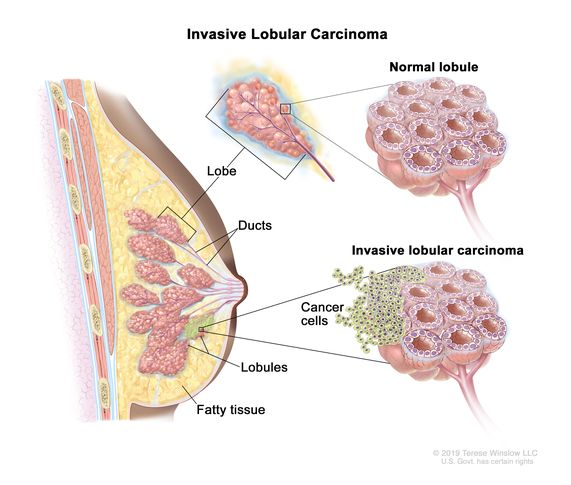
\includegraphics[width=\textwidth]{reports/assets/ilc.jpg}
		\caption{Invasive lobular carcinoma}
		\label{fig:ilc}
	\end{subfigure}
	\caption[LCIS vs. ILC comparison]{Progression from lobular carcinoma in situ (LCIS) to invasive lobular carcinoma (ILC). (a) LCIS represents abnormal cell growth restricted to the milk-producing lobules, whereas (b) ILC shows malignant cells spreading from lobules into adjacent breast tissue \cite{noauthor_nci_2011}.}
\label{fig:histological_types_two}
\end{figure}

\textbf{According to staging systems}

Clinical staging systems are a way of determining how much cancer there is and how far it has spread in the body, using tests and assessments done before surgery or other treatment. This provides standardized frameworks for prognosis and treatment planning.

\begin{itemize}
	\item \textbf{BI-RADS Staging System}: The Breast Imaging-Reporting and Data System (BI-RADS)\cite{magny_breast_2025} standardizes mammographic interpretation and assigns suspicion categories that guide medical management (see Table \ref{tab:birads_table}).
    \item  \textbf{TNM Staging System}: This is the most widely used staging system \cite{noauthor_stages_nodate}. It evaluates three key anatomical factors:
    \begin{itemize}
        \item \textbf{Tumor(T)}: Size and local extent of the primary tumor, ranging from TX (tumor cannot be assessed) to T4 (extensive local invasion).
        \item \textbf{Node(N)}: Regional lymph node involvement, from NX (nearby lymph nodes cannot be assessed) to N3 (extensive nodal spread).
        \item \textbf{Metastasis(M)}: Presence or absence of distant metastases (M0 or M1).
  \end{itemize}
  The current TNM system, updated in 2018, incorporates new parameters like estrogen receptor (ER), progesterone receptor (PR), and others clinical variables to provide more accurate prognostic stratification \cite{hortobagyi_new_2018}. 
  
\end{itemize}

\begin{table}[h!]
	\caption[Breast Imaging-Reporting and Data System (BI-RADS)]{Breast Imaging-Reporting and Data System (BI-RADS) classification \cite{noauthor_bi-rads_2025}.}
	\centering
	\begin{tabular}{lccccc}
		\toprule
		\textbf{Category} & \textbf{Definition} & \textbf{Likelihood of cancer}\\
		\midrule
		BI-RADS 0        & Incomplete                         & N/A \\
		BI-RADS 1        & Negative                           & Essentially 0\% \\
            BI-RADS 2        & Benign                             & Essentially 0\%  \\
            BI-RADS 3        & Probably benign                    & > 0\% but $\leq 2\%$ \\
            BI-RADS 4        & Suspicious                         & > 2\% but < 95 \% \\
            BI-RADS 5        & Highly suggestive of malignancy    & $\geq 95\%$ \\
            BI-RADS 6        & Known biopsy-proven malignancy     & N/A \\
		\bottomrule
	\end{tabular}
	\label{tab:birads_table}
\end{table}


In addition to these classifications, in recent years, molecular subtyping of breast cancer, based on biomarker expression and genomic profiles, has gained particular relevance, which will be addressed in the next section.


\subsection{Molecular Subtypes}

Although clinical and histological classification of breast cancer provides important information for diagnosis, it does not always allow for precise prediction of the tumor’s biological behavior or its response to specific treatments.

The research by Perou et al. (2000) \cite{perou_molecular_2000} and Sørli et al. (2003) \cite{sorlie_repeated_2003} laid the groundwork for the molecular characterization of breast cancer. Through gene expression profiling\footnote{A study that identifies which genes are active and to what extent in a cell or tissue by analyzing RNA levels produced by thousands of genes simultaneously.}, Perou et al. demonstrated that breast cancer is a heterogeneous disease and proposed a molecular subtype classification based on the genetic expression patterns of the tumors analyzed. Four subtypes were initially defined: \textbf{Luminal A}, \textbf{Luminal B}, \textbf{HER2}, and \textbf{Basal-like (Triple negative)}.

Sørli et al. reinforced these findings. They replicated the research in different patient cohorts, demonstrating that the results were not artifacts of a single study. They also showed that molecular subtypes are associated with clinically significant differences, such as prognosis and risk of distant metastasis, giving this characterization greater predictive value than traditional histological classification.

\begin{figure}
	\centering
	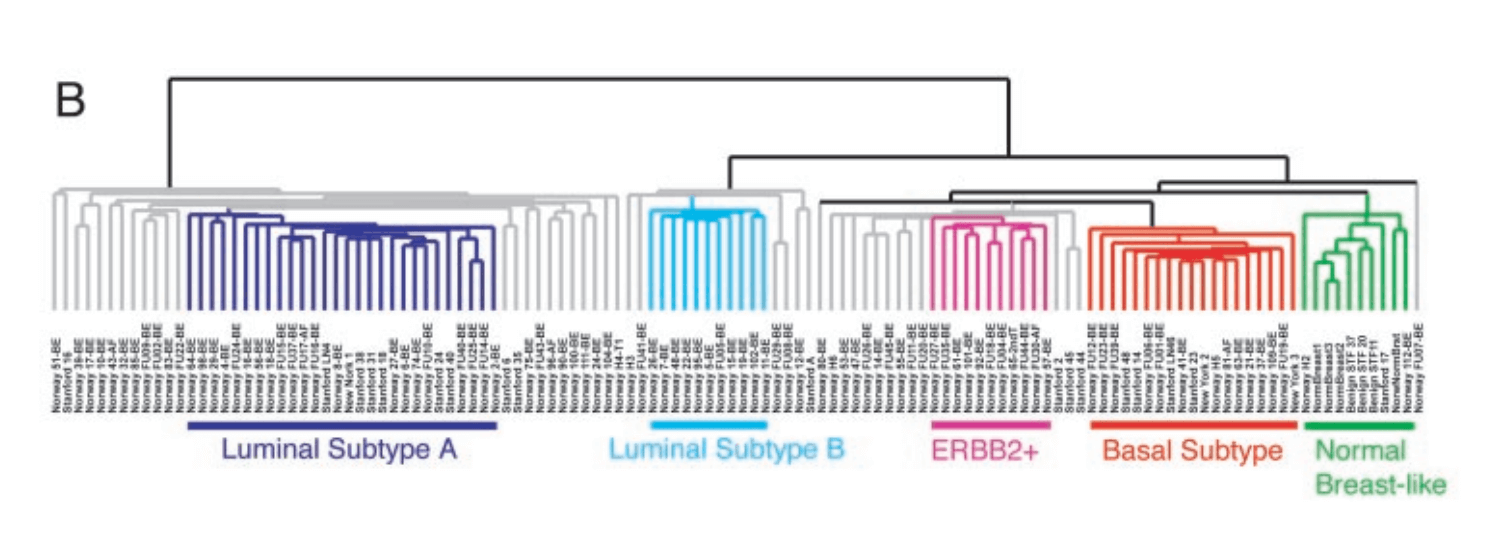
\includegraphics[width=0.8\linewidth]{reports//assets/dendogram.png}
	\caption[Molecular subtypes dendrogram by Sørli et al.]{Dendrogram from the study by Sørli et al. showing the clustering of subtypes according to genetic patterns \cite{sorlie_repeated_2003}.}
	\label{fig:sorlie-dandrogram}
\end{figure}

Following these studies, efforts focused on translating the findings into clinical practice. Since the technique used for classification at the time (DNA microarrays) was expensive, complex, and not accessible to most hospitals, an alternative was sought. It was at the St. Gallen international consensus meetings that classification criteria based on immunohistochemical (IHC) markers\footnote{Specific proteins or antigens present in cells or tissues that can be detected using antibodies in a laboratory technique called immunohistochemistry.} were proposed, formalizing the subtypes using a combination of the following hormone receptors \cite{lips_breast_2013}:

\begin{itemize}
	\item \textbf{Estrogen (ER) and Progesterone (PR) Receptors}: Define the tumor’s hormonal dependence, which can affect its growth. Tumors with these receptors respond well to hormonal therapy.
	\item \textbf{HER2 (Human epidermal growth factor receptor 2)}: A protein that stimulates cell growth. Its overexpression usually indicates a more aggressive subtype.
	\item \textbf{Ki-67}: The cell proliferation index. High Ki-67 suggests a more aggressive and rapidly proliferating tumor.
\end{itemize}

Table \ref{tab:molecular_subtypes_comb} shows these classification criteria.

\begin{table}[h!]
	\centering
        \caption[Breast cancer molecular subtypes classification criteria]{Classification criteria for molecular subtypes from the St. Gallen 2013 consensus \cite{goldhirsch_personalizing_2013}}.
	\begin{tabular}{lccccc}
		\toprule
		\textbf{Subtype} & \textbf{HER2} & \textbf{ER} & \textbf{PR} & \textbf{Ki-67} \\
		\midrule
		Luminal A        & Negative      & Positive    & Positive    & < 14\%         \\
		Luminal B/HER2-  & Negative      & Positive    & -           & $\geq$ 14\%    \\
		Luminal B/HER2+  & Positive      & Positive    & -           & -              \\
		HER2-enriched    & Positive      & Negative    & Negative    & -              \\
		Triple Negative  & Negative      & Negative    & Negative    & -              \\
		\bottomrule
	\end{tabular}
	\label{tab:molecular_subtypes_comb}
\end{table}

The Luminal A subtype is the most frequent, representing 70\% of cases at diagnosis. These tumors are characterized by slower growth and respond well to hormonal therapies, making them tumors with a better prognosis and higher survival rates. Luminal B tumors are more aggressive, have a more guarded prognosis, and are more likely to recur. They tend to be more resistant to hormonal treatments and may require chemotherapy.

HER2-enriched tumors account for 10–15\% of cases, distinguished by a rapid growth rate and overexpression of HER2, without hormone receptors. Finally, the triple negative subtype, also appearing in 10–15\% of diagnoses, lacks expression of ER, PR, and HER2. This group displays more aggressive clinical behavior, with a high rate of early recurrence and limited therapeutic options, as it does not respond to hormone therapy or targeted treatments. Conventional chemotherapy is currently the main therapeutic strategy.

\section{Medical Imaging}

Medical imaging encompasses a set of techniques and procedures used to generate visual representations of the interior of the human body for clinical and scientific purposes. These tools enable non-invasive visualization of anatomical structures and physiological processes, facilitating disease diagnosis and the study of normal and pathological anatomy.

For breast cancer diagnosis, several imaging techniques are currently employed, each with specific advantages and limitations depending on patient characteristics and clinical context, as shown in Figure \ref{fig:breast_cancer_medical}.

\begin{figure}[h!]
    \centering
    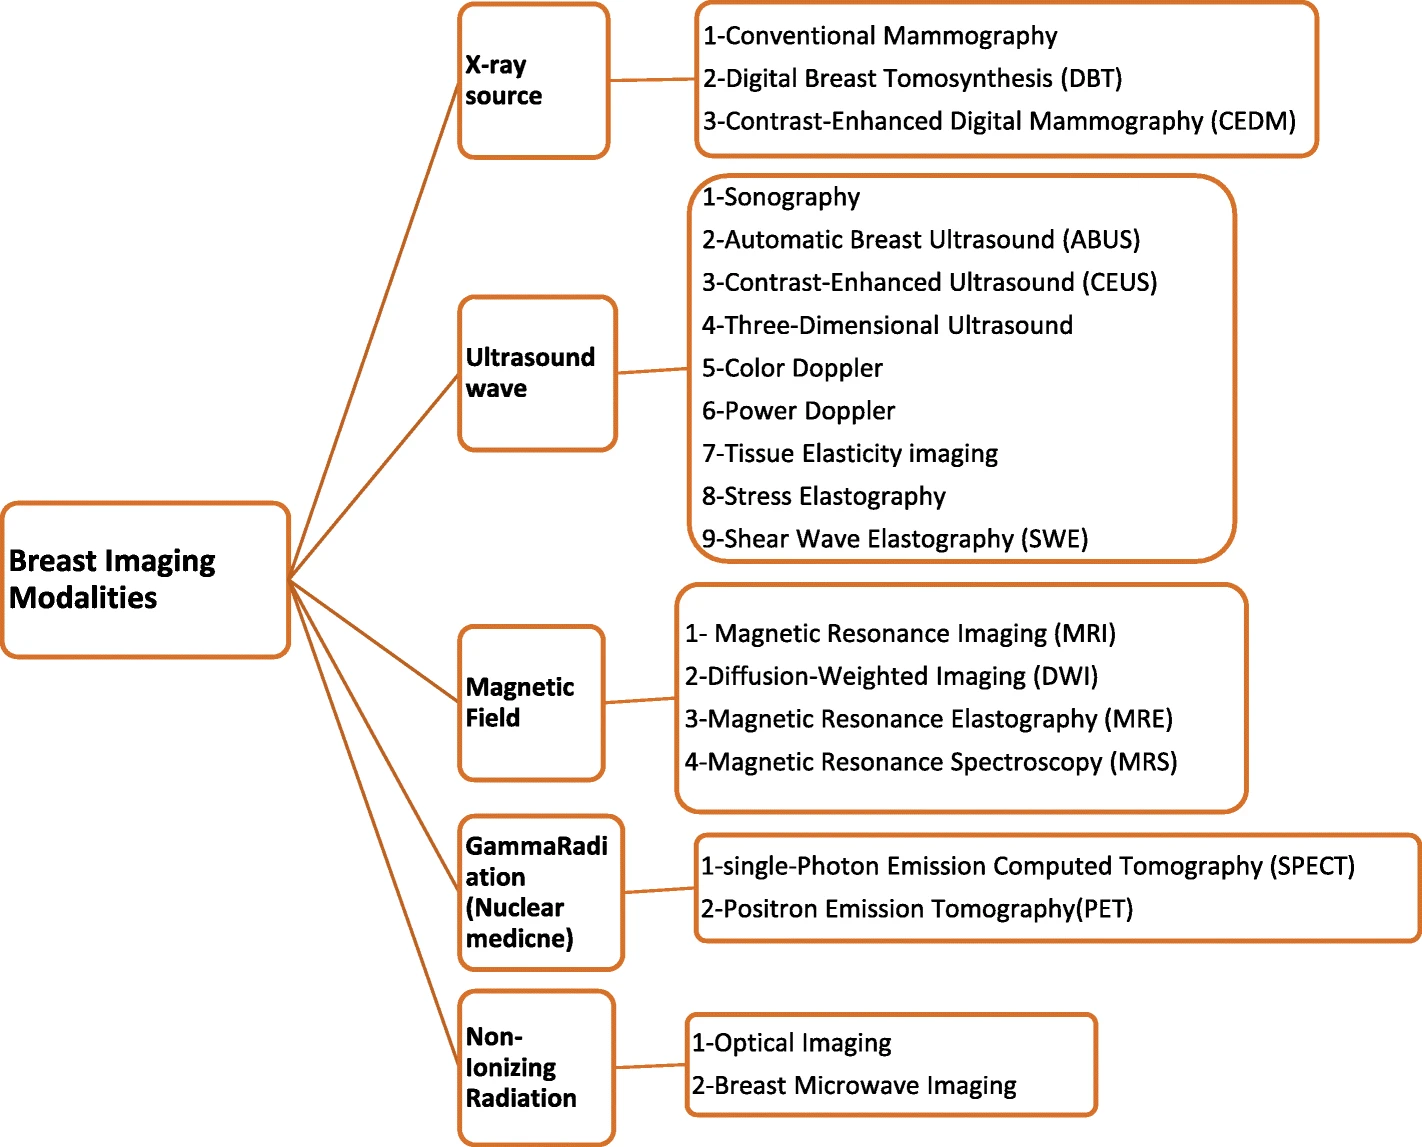
\includegraphics[width=0.75\linewidth]{reports//assets/medical_imaging.png}
    \caption[Overview of breast imaging modalities]{Overview of breast imaging modalities classified by the type of physical principle used, including x-ray, ultrasound, magnetic field, gamma radiation and non-ionizing techniques \cite{iranmakani_review_2020}.}
    \label{fig:breast_cancer_medical}
\end{figure}

\subsection{X-ray Mammography}

In this work, X-ray mammography images will be used as input to our model to infer the molecular subtype of breast cancer. As the standard imaging technique in population-based screening programs, X-ray mammography was specifically developed to examine the breast and other soft tissues. The procedure is performed using a specialized medical imaging device known as a mammography unit or mammography machine. During the exam, the breast is positioned on a flat support plate and gently compressed with a paddle. A brief burst of X-rays is then passed through the breast to a detector on the opposite side, which captures detailed images for analysis (Figure \ref{fig:mammography}).

\begin{figure}[h!]
    \centering
    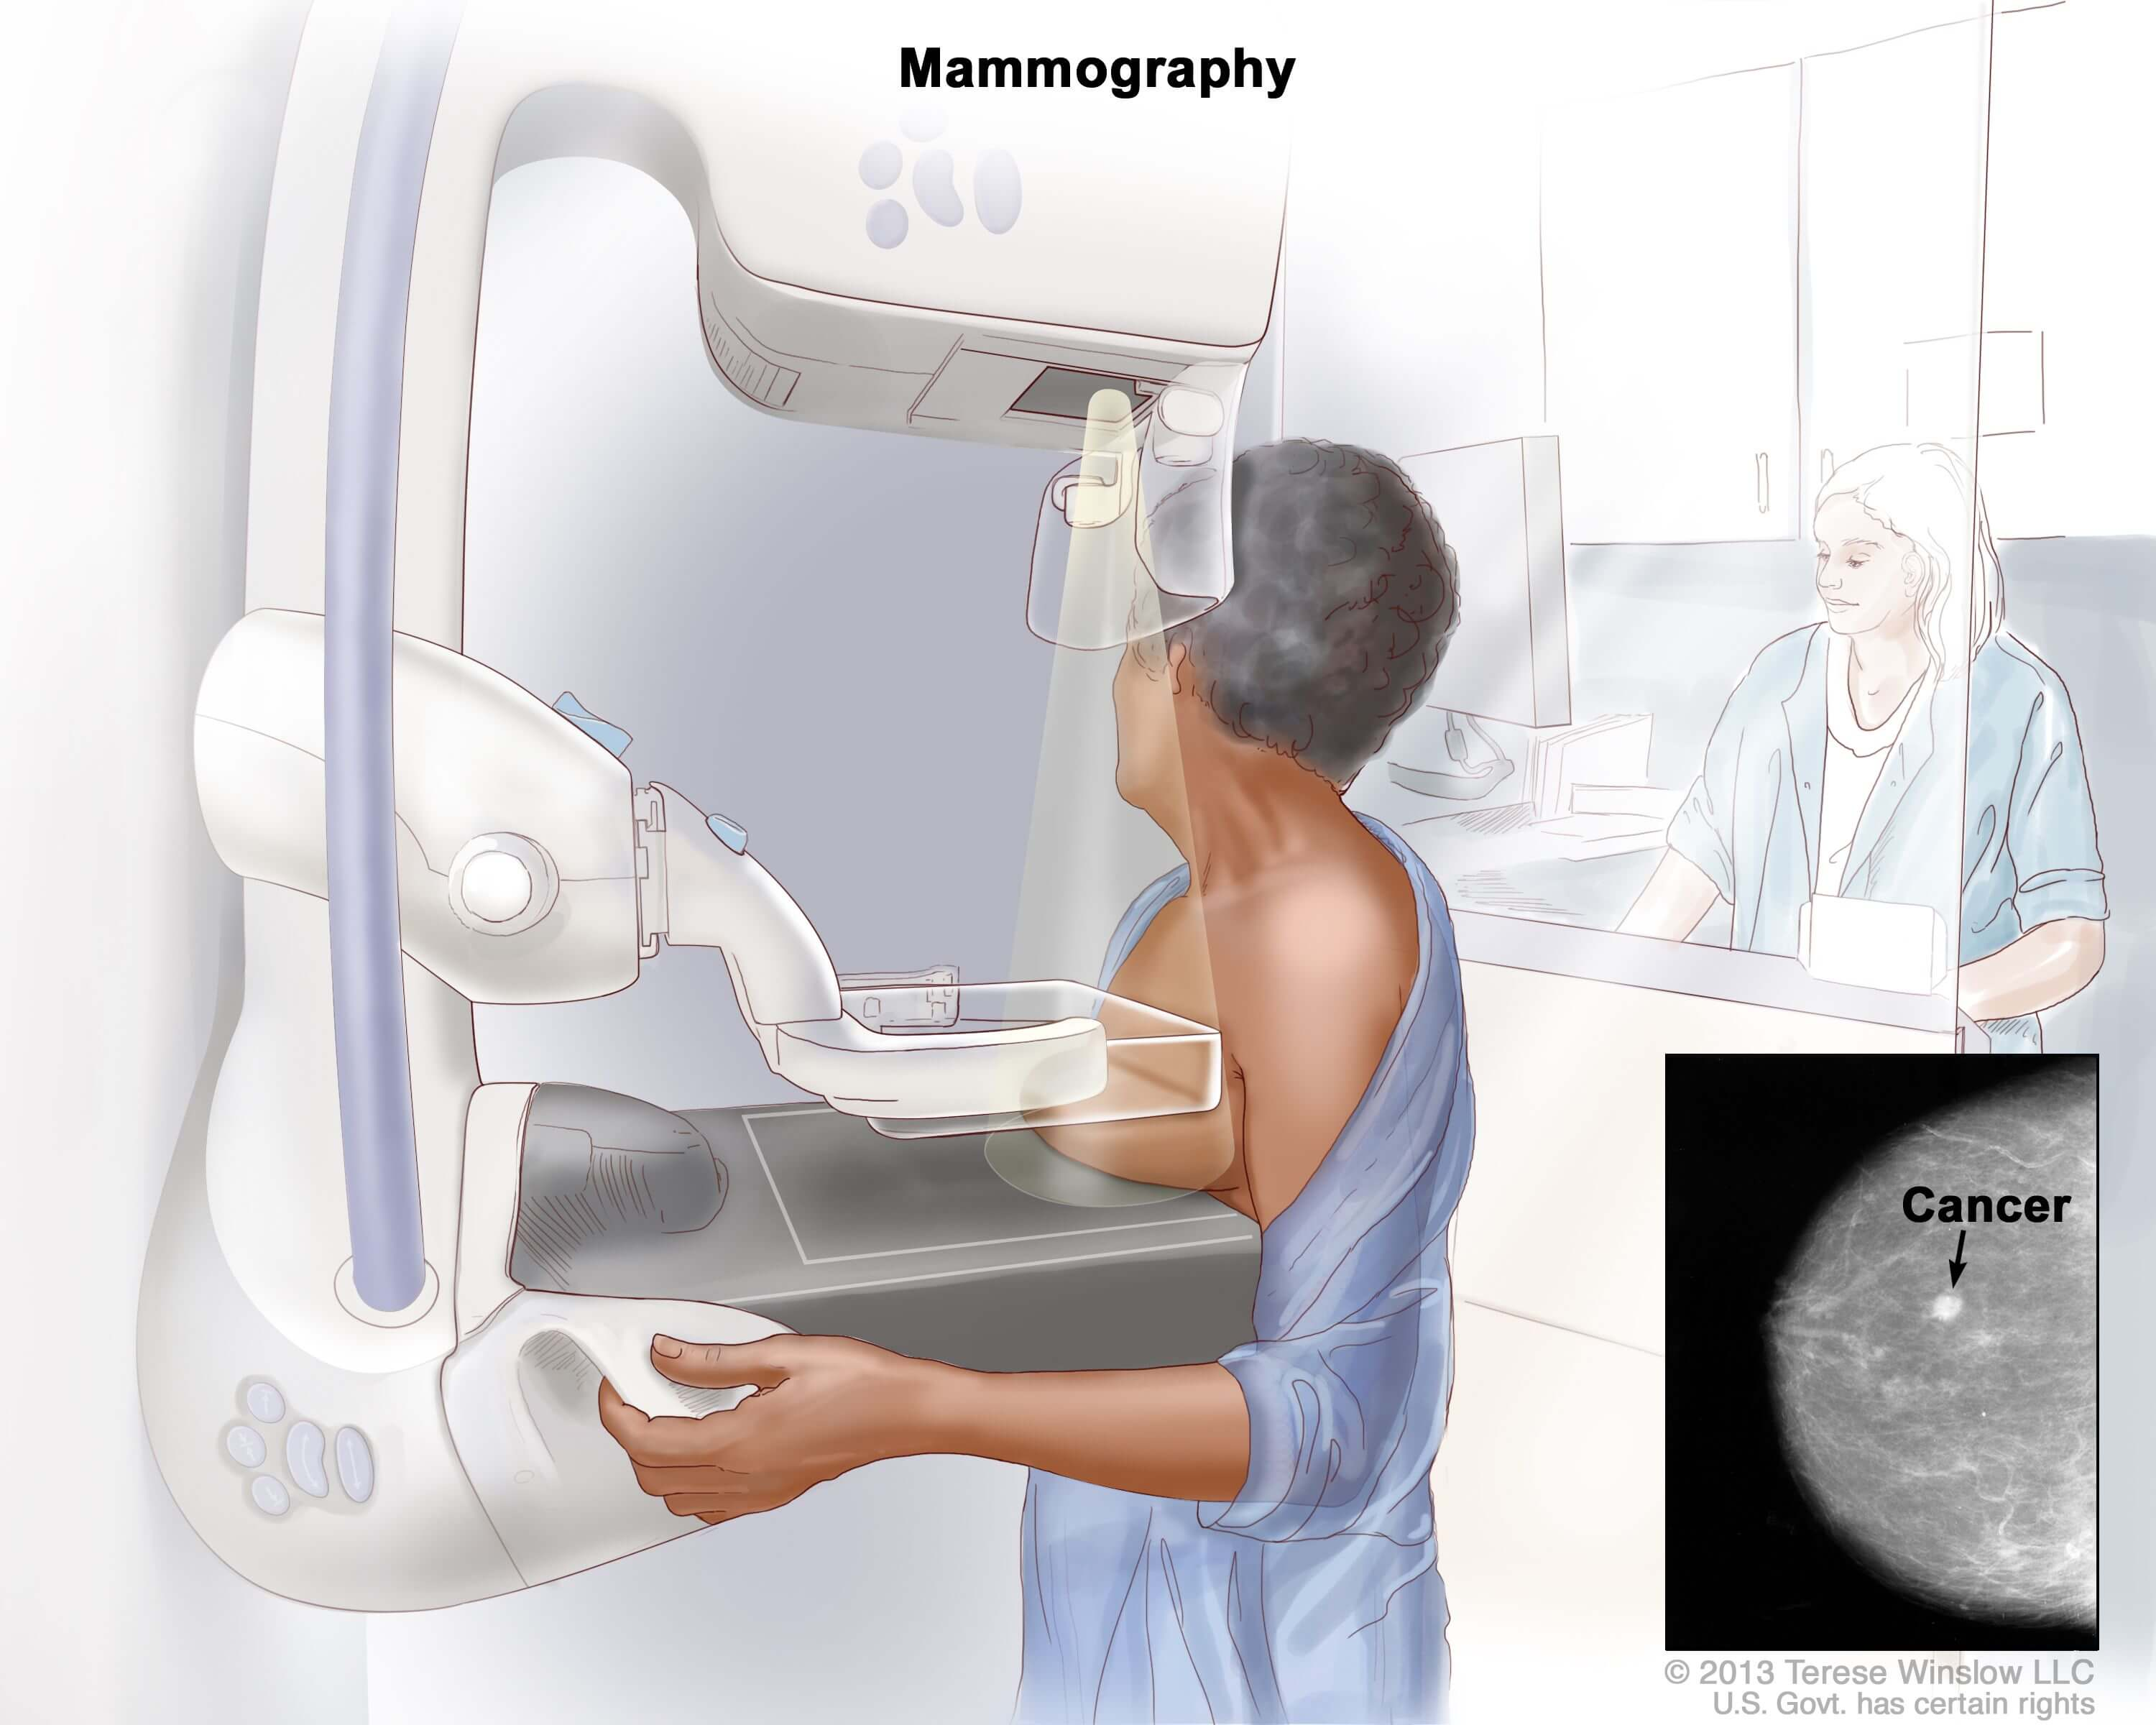
\includegraphics[width=0.45\linewidth]{reports//assets/mammography.jpg}
    \caption[Traditional mammography procedure]{Illustration showing the traditional mammography procedure \cite{nihDefinitionMammogramNCI2011}.}
    \label{fig:mammography}
\end{figure}


Each breast is typically imaged using two standard views to ensure tissue visualization:

\begin{itemize}
    \item \textbf{Craniocaudal (CC) view}: CC view is obtained from above the breast (head-to-foot) providing a top-down perspective (0º), allowing a greater visualization of the posterior and superior breast tissue. This view is particular effective for identifying whether abnormalities are located medial or lateral to the nipple \cite{noauthor_guide_nodate}.
    \item \textbf{Mediolateral oblique (MLO) view}: In the MLO view, the breast is compressed at an oblique angle (usually around 45º), enabling coverage of nearly all breast tissue \cite{noauthor_guide_nodate}. This view is particularly valuable because it includes the axillary tail and a significant portion of the pectoralis major muscle, areas where a considerable percentage (between 30\% and 40\%) of breast cancer are found \cite{aljarrah_trends_2014, noauthor_breast_2015}.
\end{itemize}



\begin{figure}[h!]
    \centering
    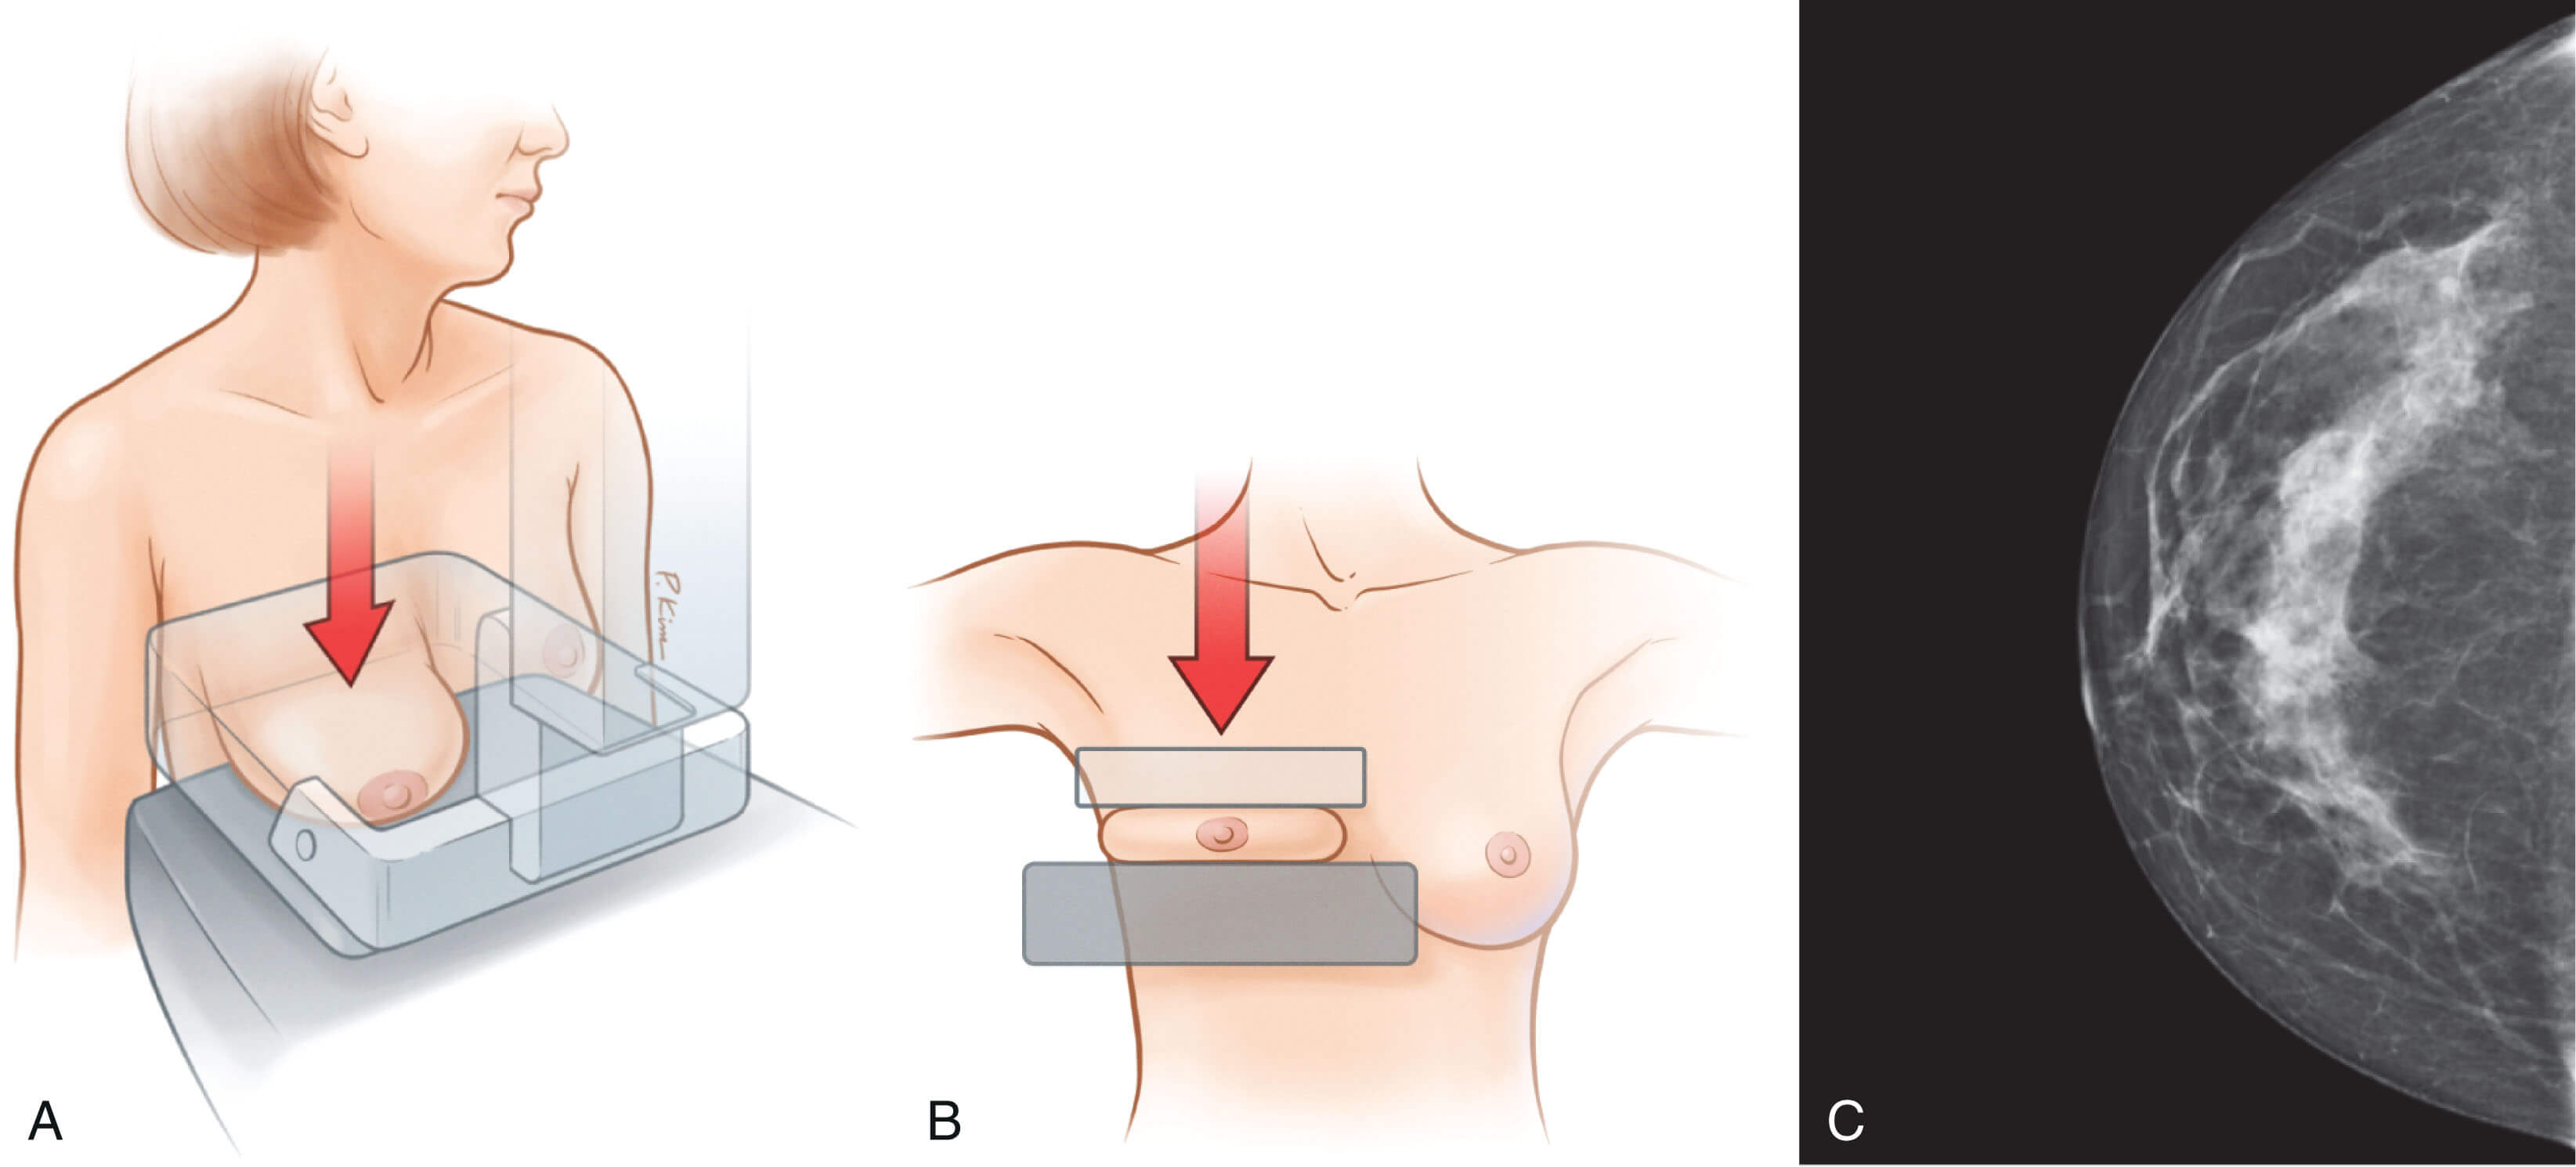
\includegraphics[width=0.6\linewidth]{reports//assets/cc_view.jpg}
    \caption[CC view acquisition procedure]{Illustration of CC view acquisition: (a) The breast is positioned horizontally on the detector and compressed with a paddle. (b) Top-down compression is applied to obtain the X-ray projection. 
    (c) Resulting mammogram image (CC view) \cite{imaging_introduction_2022}. }
    \label{fig:cc_view}
\end{figure}

\begin{figure}[h!]
    \centering
    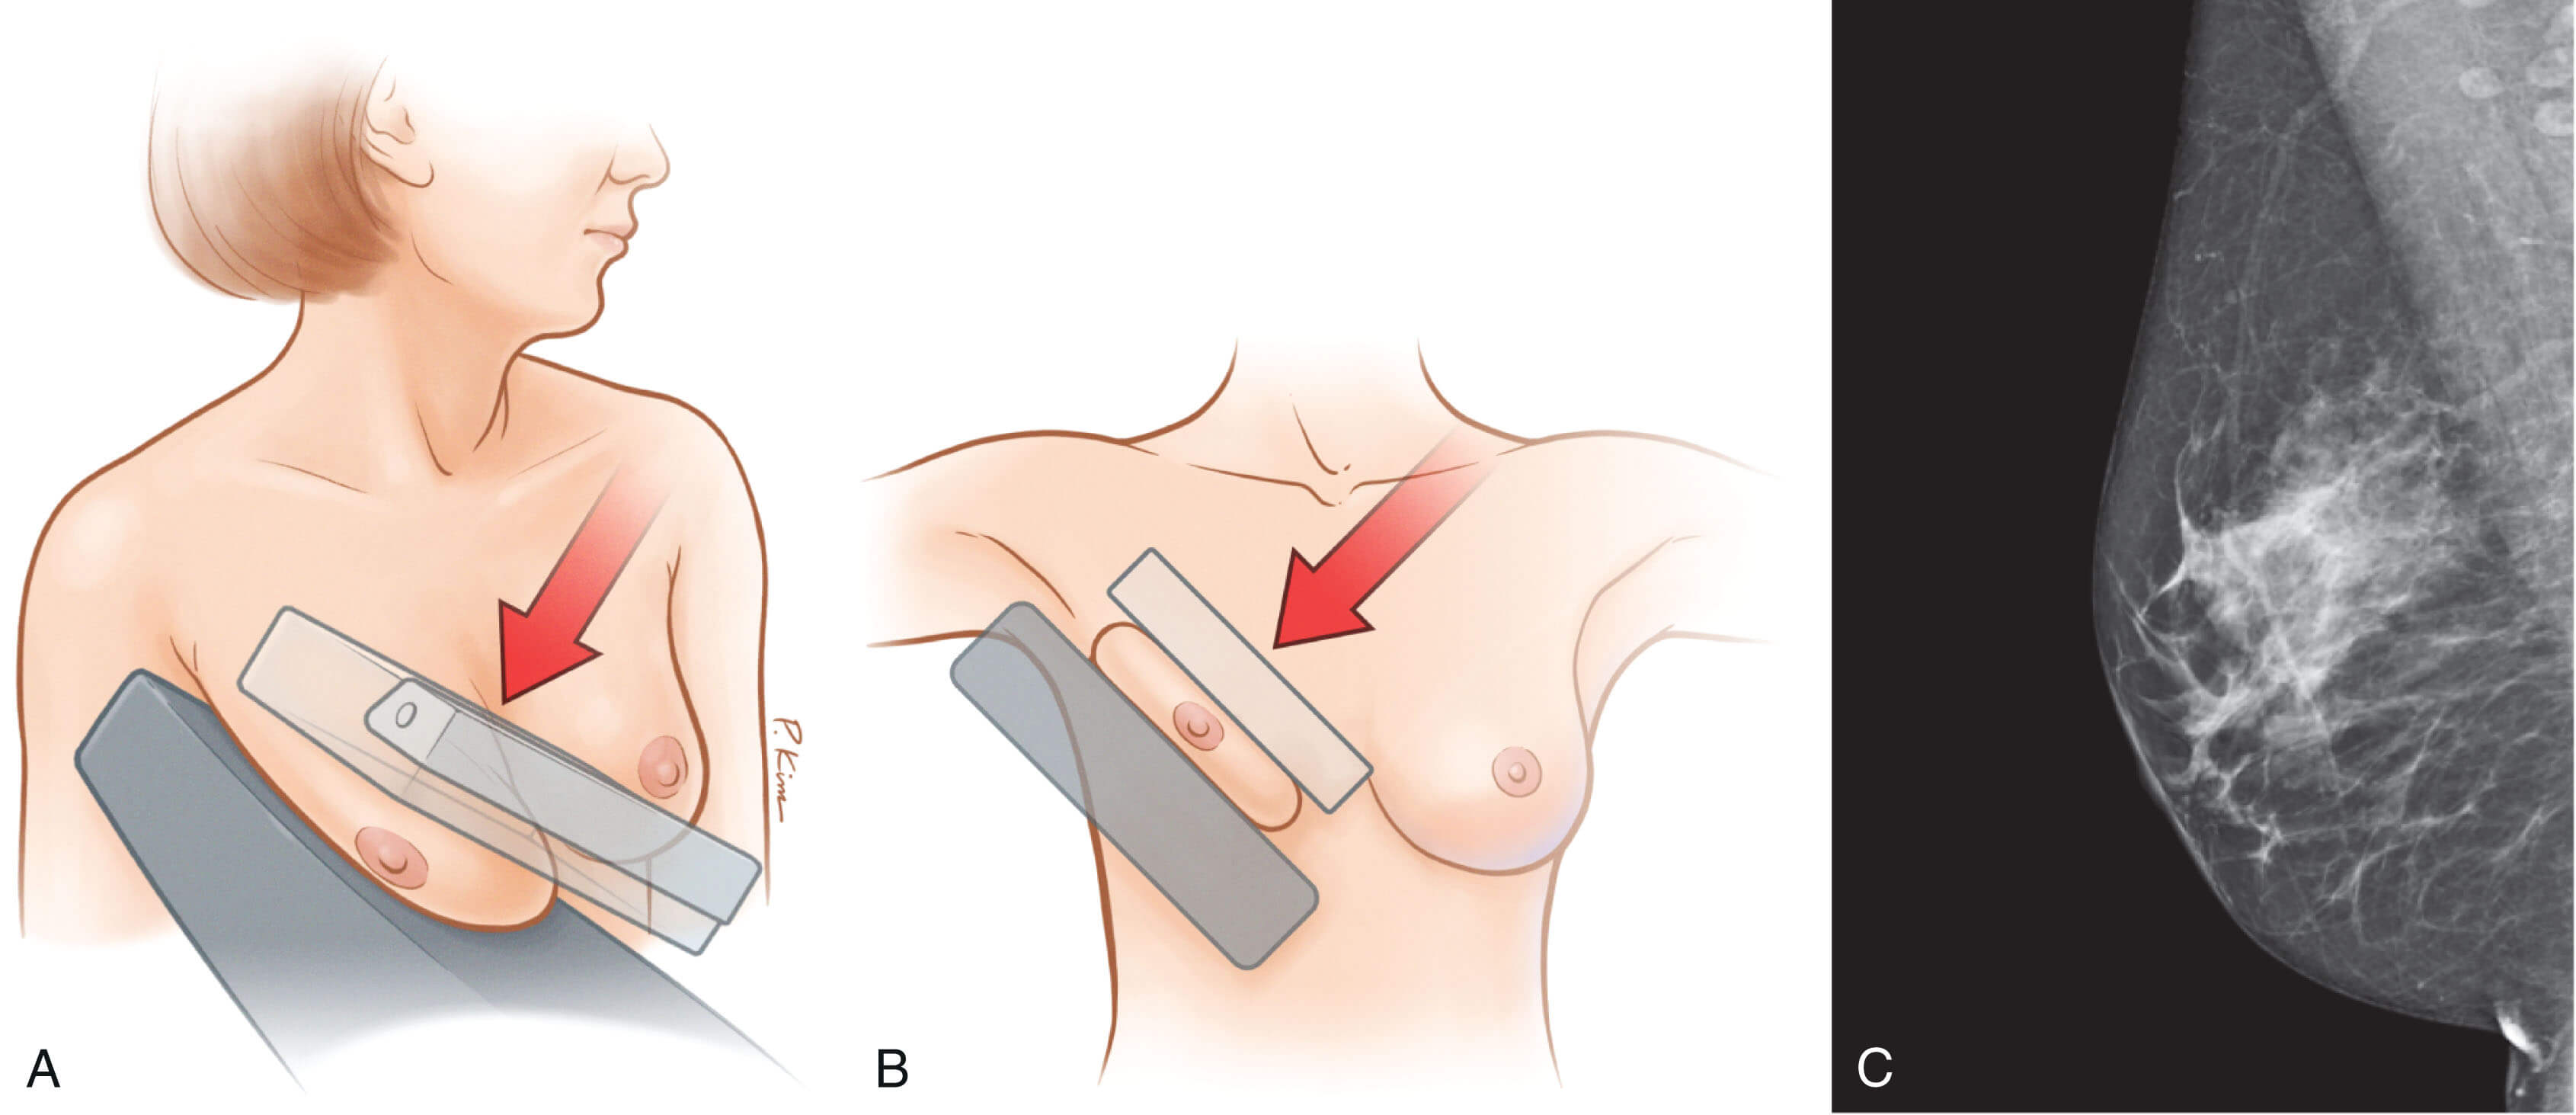
\includegraphics[width=0.6\linewidth]{reports//assets/mlo_view.jpg}
    \caption[MLO view acquisition procedure]{Illustration of MLO view acquisition: (a) The breast is positioned at an oblique angle on the detector and compressed with a paddle. (b) Compression is applied from the upper inner to the lower outer aspect to obtain the oblique X-ray projection. c) Resulting mammogram image (MLO view) \cite{imaging_introduction_2022}.}
    \label{fig:mlo_view}
\end{figure}


Modern mammography units can be either analog or digital, with digital mammography now representing the most widely used and preferred technology in clinical practice \cite{ltd_mammography_2025, noauthor_mammography_nodate}. Digital systems offer significant advantages over their analog counterparts, including immediate image acquisition, enhanced image quality, and easier storage and retrieval.

These technological advancements have further strengthened the role of mammography in clinical care. The use of x-ray mammography enables the identification of breast cancers, benign tumors, and cysts before they become palpable, often detecting tumors at a much earlier stage than physical examination alone \cite{staff_what_2025}. As a result, this technique is employed not only for routine screening in asymptomatic women, but also for diagnosing breast cancer following the detection of a lump or other symptoms, as well as for ongoing surveillance after a breast cancer diagnosis.

\subsection{Other modalities}

\textbf{Breast Ultrasound}

Breast ultrasound imaging is a widely used technique for breast analysis that uses a handheld device called a transducer\footnote{A device that produces sound waves that bounce off body tissues, receives the echoes, and transforms the signals into pictures.} to produce real-time images of the internal breast tissue by emitting high-frequency sound waves (Figure~\ref{fig:breast_ultrasound_comparison}).

Unlike mammography, ultrasound does not use ionizing radiation, making it a safe and non-invasive option for patients of all ages. This modality is particularly valuable for evaluating palpable lumps, distinguishing between solid and cystic masses, and further characterizing lesions detected on mammography, especially in women with dense breast tissue, where mammography may be less sensitive \cite{gokhale_ultrasound_2009}.

However, it is important to take into consideration that the accuracy and quality of ultrasound examinations are highly dependent on the skill and experience of the operator. In addition, compared to mammography, ultrasound is less effective at distinguishing between benign and malignant lesions, which may result in more follow-up procedures.

\begin{figure}[h!]
	\centering
	\begin{subfigure}[c]{0.45\textwidth}
		\centering
		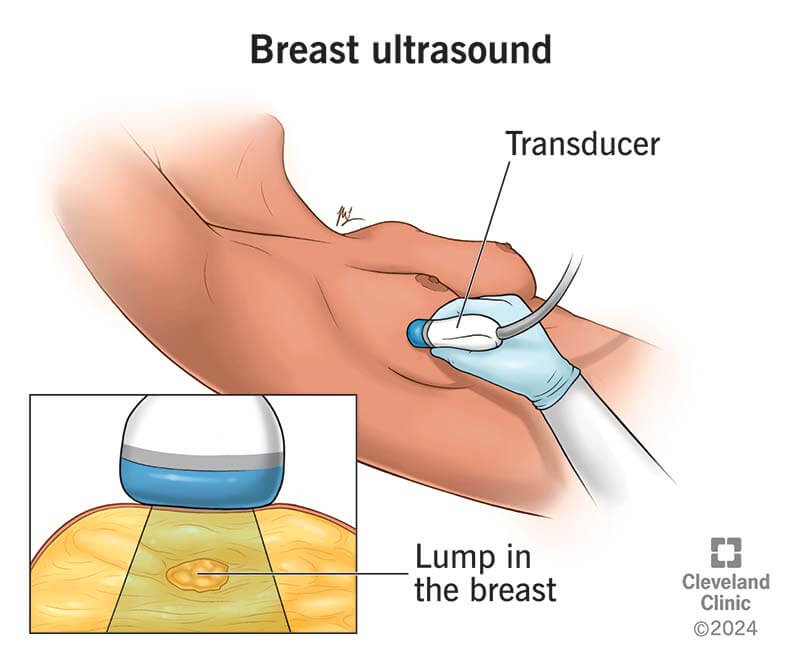
\includegraphics[width=\textwidth]{reports/assets/breast_ultrasound.jpg}
            \caption{}
		\label{fig:breast_ultrasound}
	\end{subfigure}
	\begin{subfigure}[c]{0.45\textwidth}
		\centering
		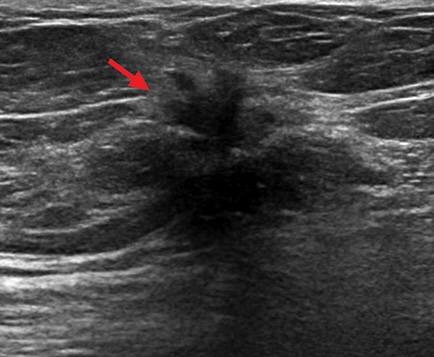
\includegraphics[width=\textwidth]{reports/assets/ultrasound.jpg}
            \caption{}
		\label{fig:ultrasound}
	\end{subfigure}
	\caption[Breast ultrasound procedure and example]{(a) Breast ultrasound representation \cite{macauley_start--finish_2022}. (b) Breast ultrasound example showing an irregular, dark gray spiculated mass, highly suspicious for cancer \cite{noauthor_breast_nodate}.}
\label{fig:breast_ultrasound_comparison}
\end{figure}

\textbf{Magnetic Resonance Imaging (MRI)}

MRI is a noninvasive imaging procedure that uses strong magnetic fields and radio waves to produce a series of highly detailed images of structures inside the body. In breast imaging, MRI operates on the same fundamental principle and is often used alongside other breast imaging modalities to detect breast cancer or other abnormalities \cite{nih_definition_2011}. 

Breast MRI is particularly valuable for women at high risk of developing breast cancer, such as those with genetic mutations or a strong family history of the disease. This is due to its high sensitivity, with detection rates exceeding 90\%, making it the most sensitive imaging modality for identifying breast cancer \cite{radswiki_breast_nodate}.

Despite these advantages, MRI is more expensive and less widely available than mammography or ultrasound. Its high sensitivity can sometimes lead to more false positives, resulting in additional follow-up imaging. Furthermore, accurate interpretation of breast MRI requires specialized training and experience \cite{noauthor_technical_nodate}.


\begin{figure}
    \centering
    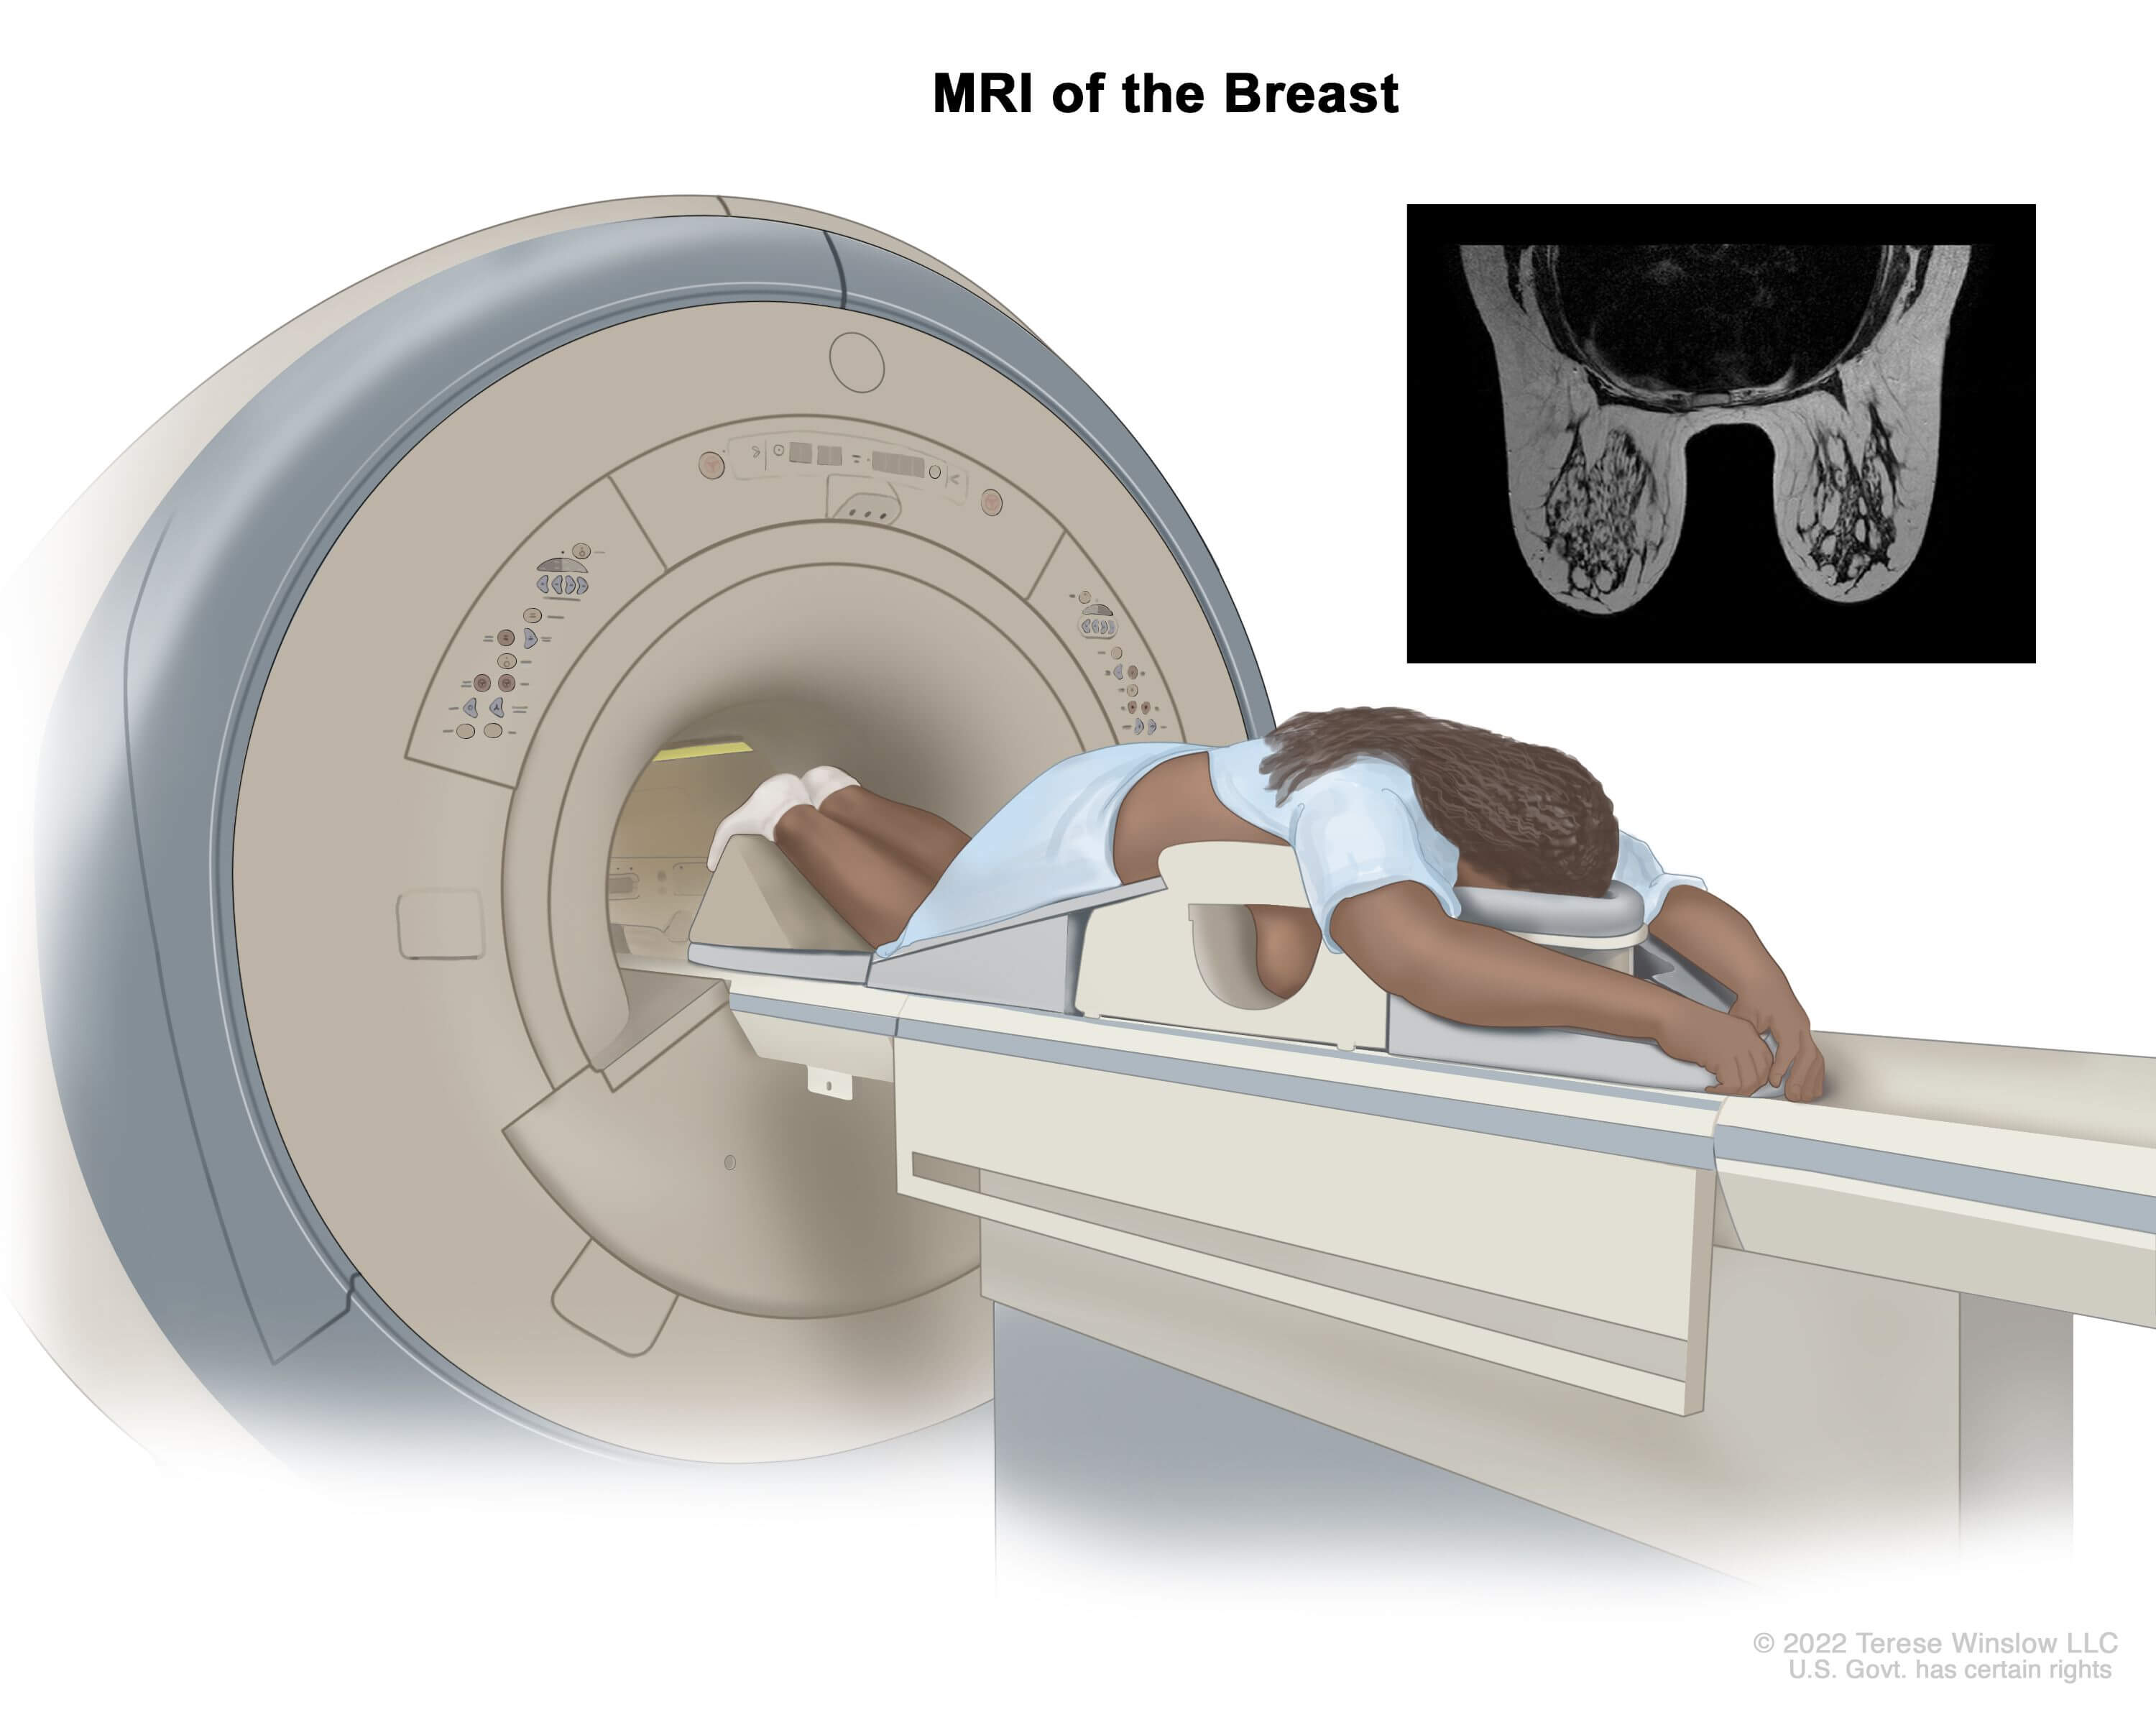
\includegraphics[width=0.5\linewidth]{reports//assets/breast_mri.jpg}
    \caption[Breast MRI procedure]{Illustration of a breast MRI procedure. The patient lies prone on a dedicated breast coil, allowing for optimal imaging of the breast tissue \cite{nih_definition_2011}.}
    \label{fig:breast_mri}
\end{figure}


\section{Cancer Screening}

Cancer screening is the process of using tests to look for cancer or pre-cancerous changes in people, mainly targeting those who do not have any symptoms of the disease. The purpose is to detect cancer at an early stage, when treatment is more likely to be successful and before symptoms appear \cite{noauthor_cancer_2010}.

There are different kinds of screening tests that can be used in the process depending on the subject’s needs. These may include physical examinations and clinical history reviews, laboratory tests, imaging procedures, and genetic tests \cite{noauthor_cancer_2010}. In the context of breast cancer, x-ray mammography is the gold-standard screening tool. As mentioned earlier, it is a widely available, noninvasive, and cost-effective technique, and it has been proven to detect tumors up to two years before they become palpable or cause symptoms \cite{cancer_que_2023}.

\subsection{General process description}

The general process of breast screening is very similar worldwide in its main steps, but certain aspects, such as the starting age, screening frequency, and technology used may vary from country to country. In Spain, the breast cancer screening program began in 1990 and is performed only in women between 50 and 69 years old, using biennial\footnote{Every two years} mammograms \cite{noauthor_ministerio_nodate}. The following steps are the core steps of breast cancer screening:

\begin{enumerate}
    \item \textbf{Invitation}: Eligible women (based on age and sometimes risk factors) are invited to participate, either through organized national programs or through healthcare providers.
    \item \textbf{Screening test}: The screening test is performed, typically a mammogram, which may be supplemented by other tests. For example, in Spain, an ultrasound is also recommended \cite{noauthor_map_nodate}.
    \item \textbf{Image review}: Radiologists review the mammograms for signs of cancer, such as masses or microcalcifications.
    \item \textbf{Results notification}: Women are informed of their results. Those with abnormal findings are called back for additional tests.
    \item \textbf{Follow-up}: If abnormalities are detected, further diagnostic procedures, such as additional imaging or biopsy, are conducted to confirm or rule out cancer.
\end{enumerate}


At this stage, non-invasive techniques, such as those investigated in this work, can contribute to improved diagnostic outcomes and offer more detailed insights. Specifically, in the context of molecular subtype classification, having such a tool would provide additional information for cases with abnormal findings or confirmed cancers. This could lead to a better prognosis and help guide clinical decision-making, potentially reducing the need for further invasive procedures like biopsies.

\subsection{Biopsy Techniques}

When imaging or other screening tests detect abnormalities suggestive of breast cancer, a biopsy is typically required to obtain a definitive diagnosis. A breast biopsy involves removing a small sample of tissue from the suspicious area, which is then examined under a microscope by a pathologist \cite{DefinitionBiopsyNCI2011}. This step is crucial not only for confirming the presence of cancer but also for determining its type, grade, and increasingly, its molecular characteristics.

\textbf{Classification}

Several biopsy techniques are commonly used for the diagnosis and characterization of breast lesions, including:

\begin{itemize}
    \item \textbf{Fine Needle Aspiration (FNA)}: A minimally invasive procedure that uses a thin, hollow needle to extract cells or fluid from a suspicious area. It is often performed when the lesion is likely to be a cyst\footnote{A fluid-filled sac}. FNA is quick, cost-effective, and generally well-tolerated, offering high diagnostic accuracy when performed correctly. However, it may provide limited information about tissue structure and can sometimes yield inconclusive results, requiring further evaluation with a core needle or surgical biopsy \cite{noauthor_fine_nodate, silva_breast_2023}.
    
    \item \textbf{Core Needle Biopsy (CNB)}: This technique employs a larger, hollow needle to obtain small cylinders (cores) of tissue, usually under image guidance \cite{CoreNeedleBiopsy, silva_breast_2023}. CNB yields a larger tissue sample, allowing for accurate histological diagnosis and molecular marker assessment, both of which are essential for molecular subtyping. It is considered the standard diagnostic approach due to its high concordance with surgical specimens for key biomarkers such as ER, PR, HER2, and Ki67 \cite{jeong_analysis_2020}.
    
    \item \textbf{Vacuum-Assisted Biopsy (VAB)}: VAB uses a vacuum-powered device to collect multiple tissue samples through a single insertion, typically guided by stereotactic\footnote{A surgical technique or procedure that uses a three-dimensional coordinate system to precisely locate and target a specific area.} or ultrasound imaging. It is particularly effective for sampling microcalcifications or small lesions detected via mammography and yields larger tissue samples, thereby reducing sampling error. This method is reliable, well-tolerated, and can sometimes eliminate the need for surgical biopsy, especially for benign lesions \cite{park_vacuum-assisted_2014}.
    
    \item \textbf{Surgical Biopsy}: When needle-based techniques are inconclusive or not feasible, a surgical biopsy may be performed to excise part or all of the suspicious tissue. While it provides the most comprehensive tissue sample, it is also more invasive and costly, and is generally reserved for cases where less invasive methods fail to yield a definitive diagnosis \cite{silva_breast_2023}.
\end{itemize}

\textbf{Limitations}

The choice of biopsy technique is influenced by factors such as lesion size, location, imaging characteristics, and patient-specific considerations. Although biopsy remains the gold standard for cancer diagnosis, it is associated with several significant limitations, including:

\begin{itemize}
    \item \textbf{Invasiveness}: The procedure may cause discomfort and carries a potential risk of infection or bleeding, particularly when tumors are located in hard-to-reach areas \cite{amino_pros_2024}.
    \item \textbf{Logistical Barriers}: In resource-limited settings, a lack of trained personnel and the need for patients to travel long distances for care can hinder timely diagnosis and treatment \cite{silva_breast_2023}.
    \item \textbf{Inconclusive Results}: If not performed by experienced personnel, biopsies can yield insufficient or non-diagnostic samples, increasing patient burden and discomfort due to the need for repeat procedures.
\end{itemize}

Given these limitations, there is a clear need for developing non-invasive diagnostic approaches. Such techniques could facilitate earlier intervention, reduce the dependence on tissue sampling, and improve access to timely and accurate diagnosis, especially in settings where biopsy is not feasible.


\chapter{Technological Review}

This section explores the modern definitions and structures of AI models, as well as their use in modern medicine and specifically in medical imaging.

\section{Artificial Intelligence}

Artificial Intelligence (AI) refers to a collection of technologies that allow computers and machines to mimic human intelligence, including learning, problem-solving, and decision-making with varying levels of creativity and autonomy \cite{colestrykerWhatArtificialIntelligence2024}. The conceptual roots of AI can be traced back to the 1940s and 1950s, when pioneers like Alan Turing explored the idea of machines simulating human thought. Turing’s work, including the influential “Turing Test” and his 1950 paper, laid the groundwork for the field \cite{turing_icomputing_1950}. AI was formally established as a discipline in 1956 at the Dartmouth Conference, where the term “artificial intelligence” was introduced by John McCarthy, Marvin Minsky, Nathaniel Rochester, and Claude Shannon \cite{filipsson_evolution_2024}. Figure \ref{fig:ai_timeline} summarizes the evolution of AI over the decades and highlights key milestones in its development.

\begin{figure}[h!]
\centering
\begin{chronology}*[5]{1949}{2025}{\textwidth}
  \event{1950}{\footnotesize Turing's test proposal}
  \event{1956}{\footnotesize Dartmouth: term \textit{AI} coined}
  \event{1965}{\footnotesize Expert systems}
  \event[1974]{1980}{\footnotesize First AI Winter}
  \event{1986}{\footnotesize Backpropagation introduced}
  \event[1987]{1993}{\footnotesize Second AI Winter}
  \event{2012}{\footnotesize DL revolution}
  \event{2020}{\footnotesize Vision Transformers}
\end{chronology}
\caption[AI Timeline]{Condensed timeline of key AI milestones}
\label{fig:ai_timeline}
\end{figure}


\subsection{Classical AI}

The early years of artificial intelligence focused on explicit programming and rule-based systems, known as expert systems, which aimed to mimic human problem-solving. Notable examples include Dendral, used for chemical structure analysis, and Mycin, developed for diagnosing bacterial infections and suggesting treatments. These systems, developed in the 1960s and 1970s, demonstrated the promise of AI in fields like medicine and scientific research \cite{filipsson_evolution_2024}.

However, rule-based approaches soon revealed significant limitations, such as their inability to adapt to new information or handle complex, unstructured data. Combined with limited computational resources and unrealistic expectations, these challenges led to periods of stagnation in AI research, known as “AI winters.” The field eventually revived as digital data became more widely available and new AI paradigms emerged.

\subsection{Machine Learning}

Machine Learning (ML) is a branch of artificial intelligence that enables computers to learn from data and experience, allowing them to recognize patterns, make inferences, and predict outcomes without explicit rule-based programming \cite{noauthor_what_nodate}. Its rapid growth has been driven by the explosion of big data, advances in computational resources, and the availability of large annotated datasets. ML encompasses several main learning paradigms:

\begin{itemize}
\item \textbf{Supervised Learning}: Models are trained on labeled data, where each input is paired with a known output, enabling the model to learn the mapping between them \cite{jiang_supervised_2020}.
\item \textbf{Unsupervised Learning}: Models work with unlabeled data, aiming to discover hidden patterns or structures within the dataset \cite{noauthor_unsupervised_nodate}.
\item \textbf{Reinforcement Learning}: Models learn by interacting with an environment, receiving feedback through rewards or penalties, and gradually improving their decision-making strategies \cite{ghasemi_introduction_2024}.
\end{itemize}



The adoption of ML has had a transformative impact across numerous industries. In healthcare, ML models now assist in tasks ranging from automated medical image analysis to personalized treatment recommendations. The rapid advancement of ML applications, combined with the explosion of available data and improvements in hardware (such as GPUs), paved the way for the next major leap in AI: deep learning (DL).


\subsection{Deep Learning}

DL is a specialized subset of ML that utilizes artificial neural networks (ANN) composed of multiple layers to automatically extract complex features from large datasets. This approach has enabled unprecedented performance in fields such as image analysis, speech recognition, and natural language processing  \cite{holdsworthWhatDeepLearning2024}.

Unlike traditional ML methods, which often rely on manual feature engineering and are best suited for structured, moderate-sized datasets, DL models excel at processing vast amounts of unstructured data, including images, audio, and text. These models are capable of autonomously learning hierarchical representations directly from raw inputs, significantly reducing the need for human intervention and enhancing both scalability and accuracy \cite{holdsworthWhatDeepLearning2024}. Figure~\ref{fig:ai_overview} illustrates how DL fits within the broader context of AI and ML.

\begin{figure}[h!]
    \centering
    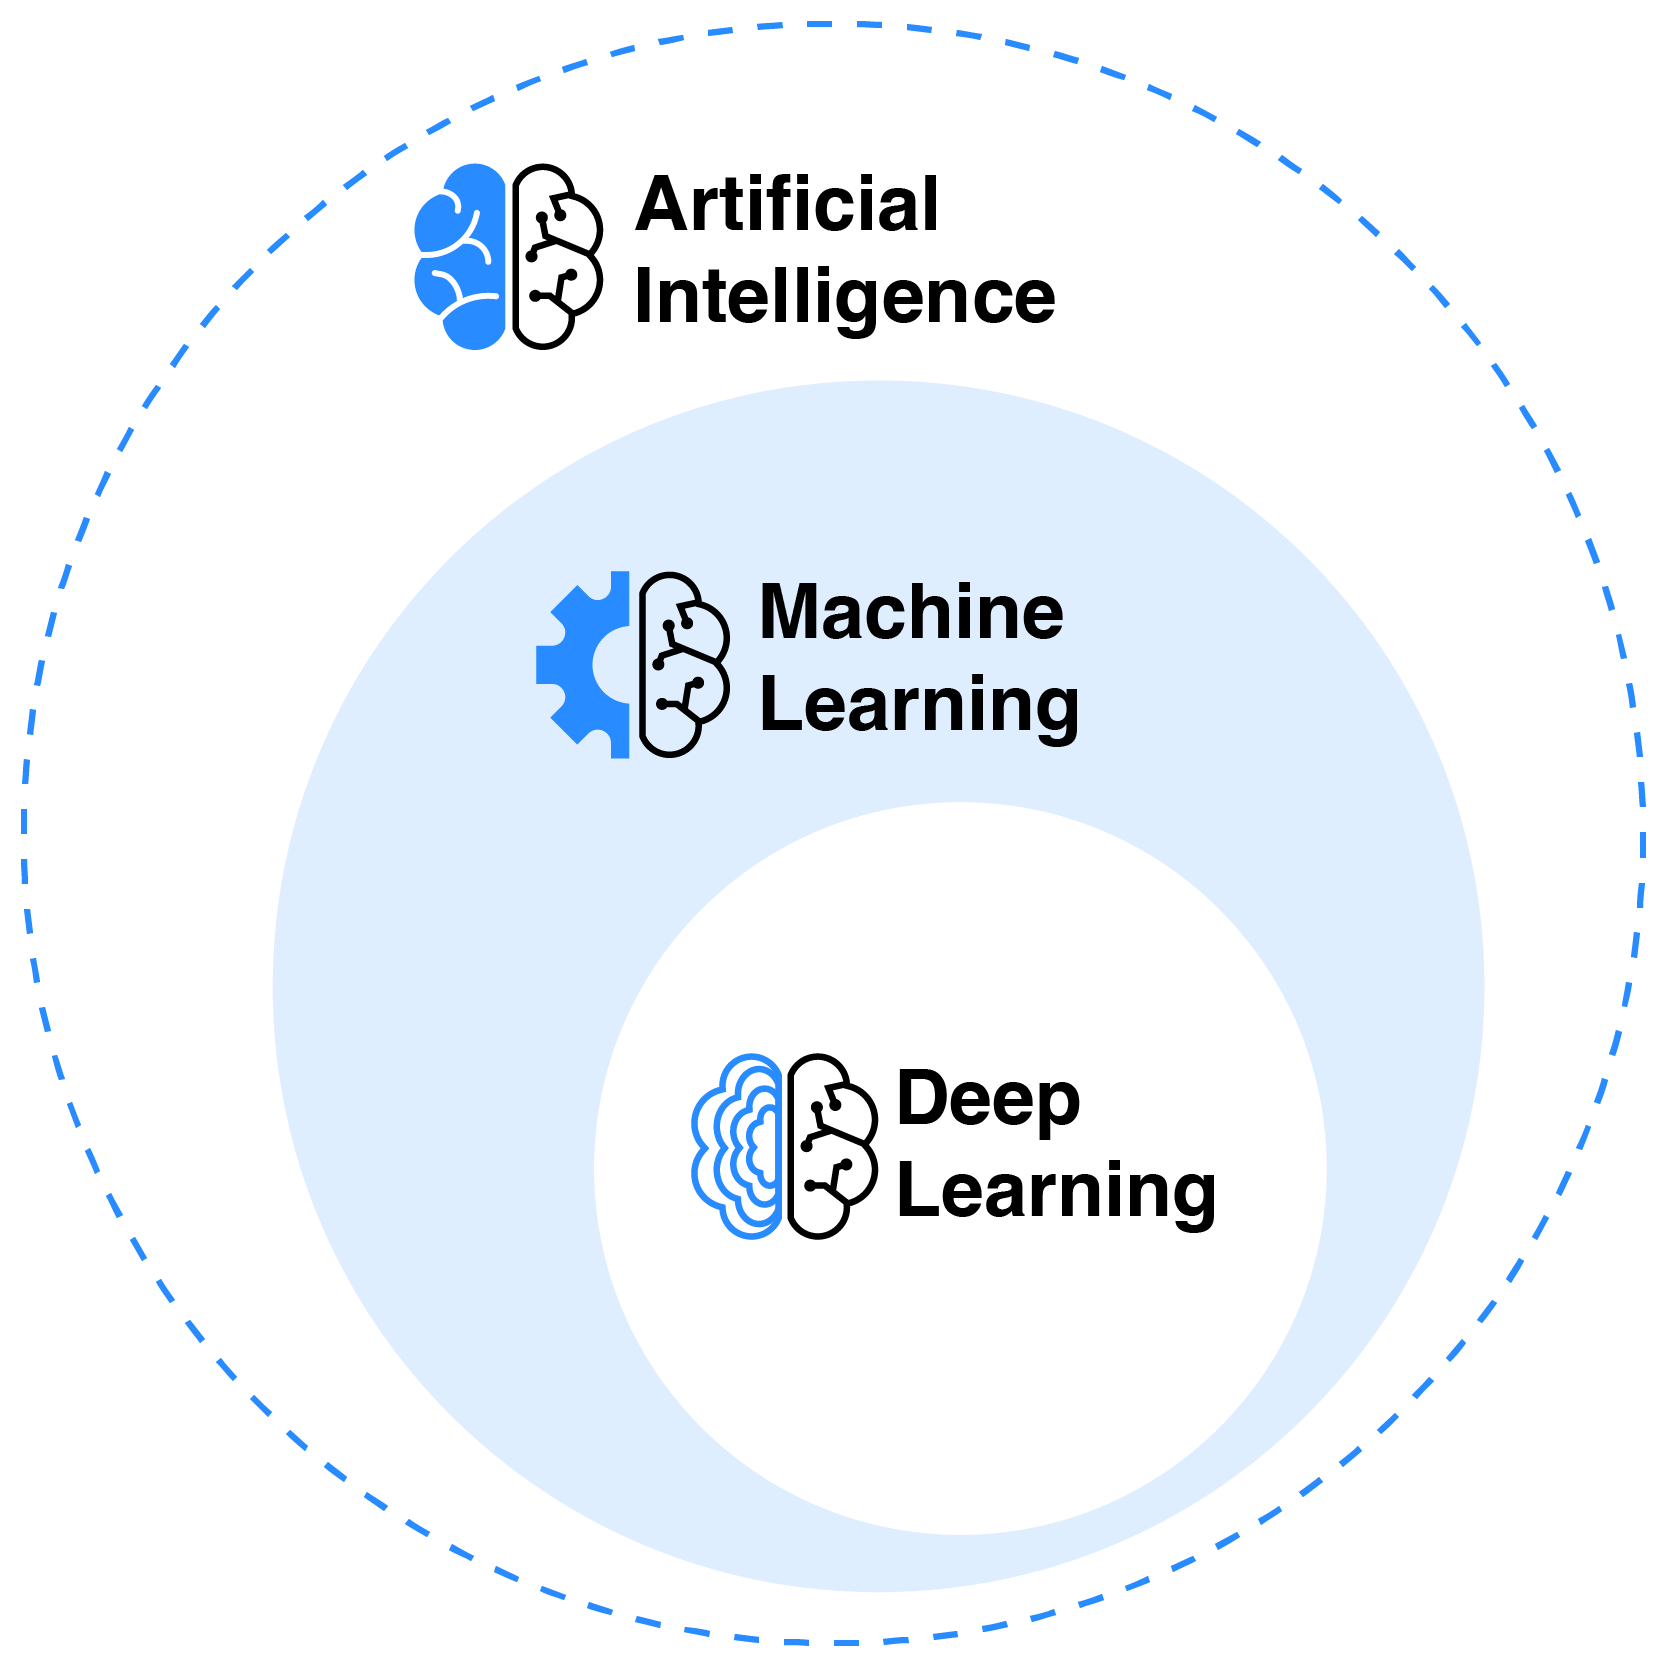
\includegraphics[width=0.5\linewidth]{reports//assets/ai.png}
    \caption[AI subsets overview]{Overview of AI subsets \cite{nasaWhatArtificialIntelligence}.}
    \label{fig:ai_overview}
\end{figure}


\subsection{Deep Learning in Medical Imaging}

The advent of DL techniques has profoundly transformed the field of medical imaging, enabling highly accurate analysis of complex visual data across a broad spectrum of clinical applications, including:

\begin{itemize}
    \item \textbf{Image classification and detection}: DL models are trained to identify and classify abnormalities in radiological images such as X-rays, MRI, or mammograms, often achieving expert-level performance.
    \item \textbf{Segmentation}: DL architectures facilitate the precise delineation of anatomical structures and pathological regions, which is essential for treatment planning, diagnosis, and disease monitoring.
    \item \textbf{Image enhancement and generation}: DL is employed to improve image quality (e.g., denoising, super-resolution) and to generate synthetic data for augmentation or cross-modality image synthesis.
\end{itemize}

These advancements have been largely driven by the success of Convolutional Neural Networks (CNNs), which have become the foundation of most state-of-the-art models in medical image analysis. CNN-based models are currently being actively explored for the classification of breast cancer molecular subtypes using mammography images, as recent studies have demonstrated their potential for this challenging task\cite{mota_breast_2024, ben_rabah_multimodal_2025}. For this reason, CNNs, particularly ResNet101, serve as the baseline architecture in this study. A detailed review of CNNs will be provided in the following section.



\section{Convolutional Neural Networks}

A Convolutional Neural Network (CNN) is a type of DL model designed to automatically learn features from data, especially images, using convolution operations. First introduced by LeCun et al. for digit recognition \cite{lecun_gradient-based_1998} with the LeNet architecture (Figure \ref{fig:lenet}). CNNs became widely adopted after the success of AlexNet in the 2012 ImageNet competition \cite{NIPS2012_c399862d}. Their main advantage is the ability to learn hierarchical features directly from raw data, reducing the need for manual feature extraction and enabling strong performance in computer vision tasks.

\begin{figure}[h!]
    \centering
    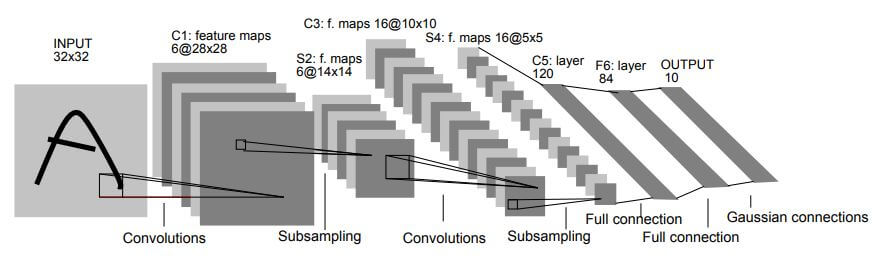
\includegraphics[width=0.8\linewidth]{reports//assets/lenet.jpg}
    \caption[LeNet CNN]{LeNet, considered the first CNN architecture for digit recognition \cite{lecun_gradient-based_1998}.}
    \label{fig:lenet}
\end{figure}


\subsection{Core Components}

\textbf{Convolutional Layers}

A convolutional layer is a core part of a CNN that scans the input image with small filters (kernels), performing a convolution operation, essentially a sliding dot product between the filter and local image regions. This process creates feature maps that emphasize important patterns, such as edges or textures \cite{noauthor_what_2021}. These feature maps are then passed through additional layers to extract more complex features. Figure \ref{fig:convolution_feature_map} illustrates the convolution operation and a feature map example of a breast image.

\begin{figure}[h!]
	\centering
	\begin{subfigure}[c]{0.45\textwidth}
		\centering
		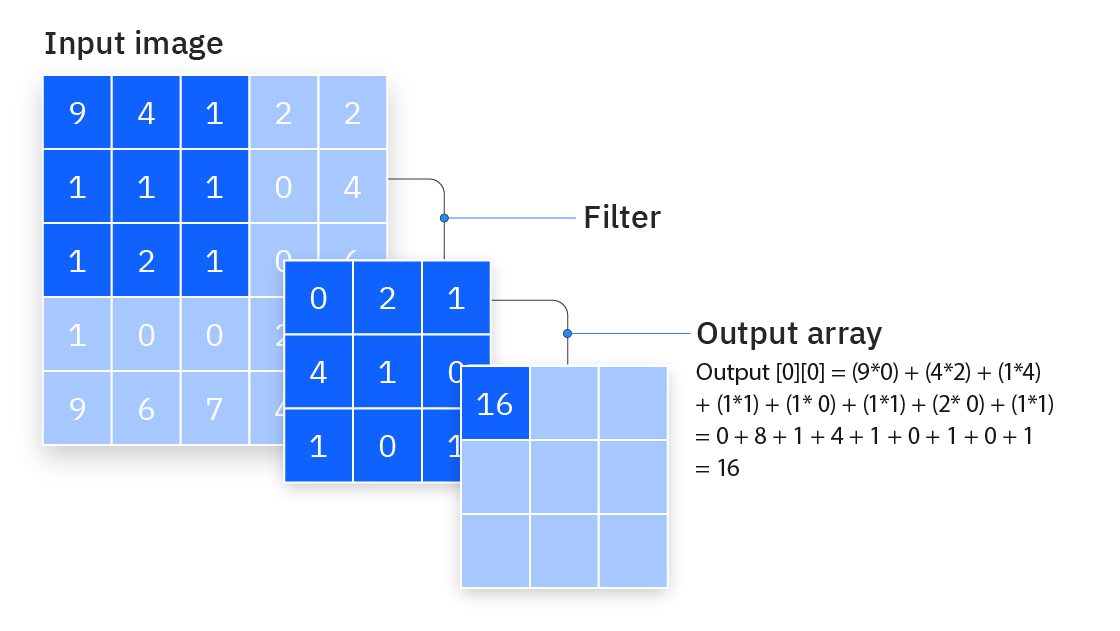
\includegraphics[width=\textwidth]{reports/assets/convolution.png}
            \caption{}
		\label{fig:convolution}
	\end{subfigure}
	\begin{subfigure}[c]{0.25\textwidth}
		\centering
		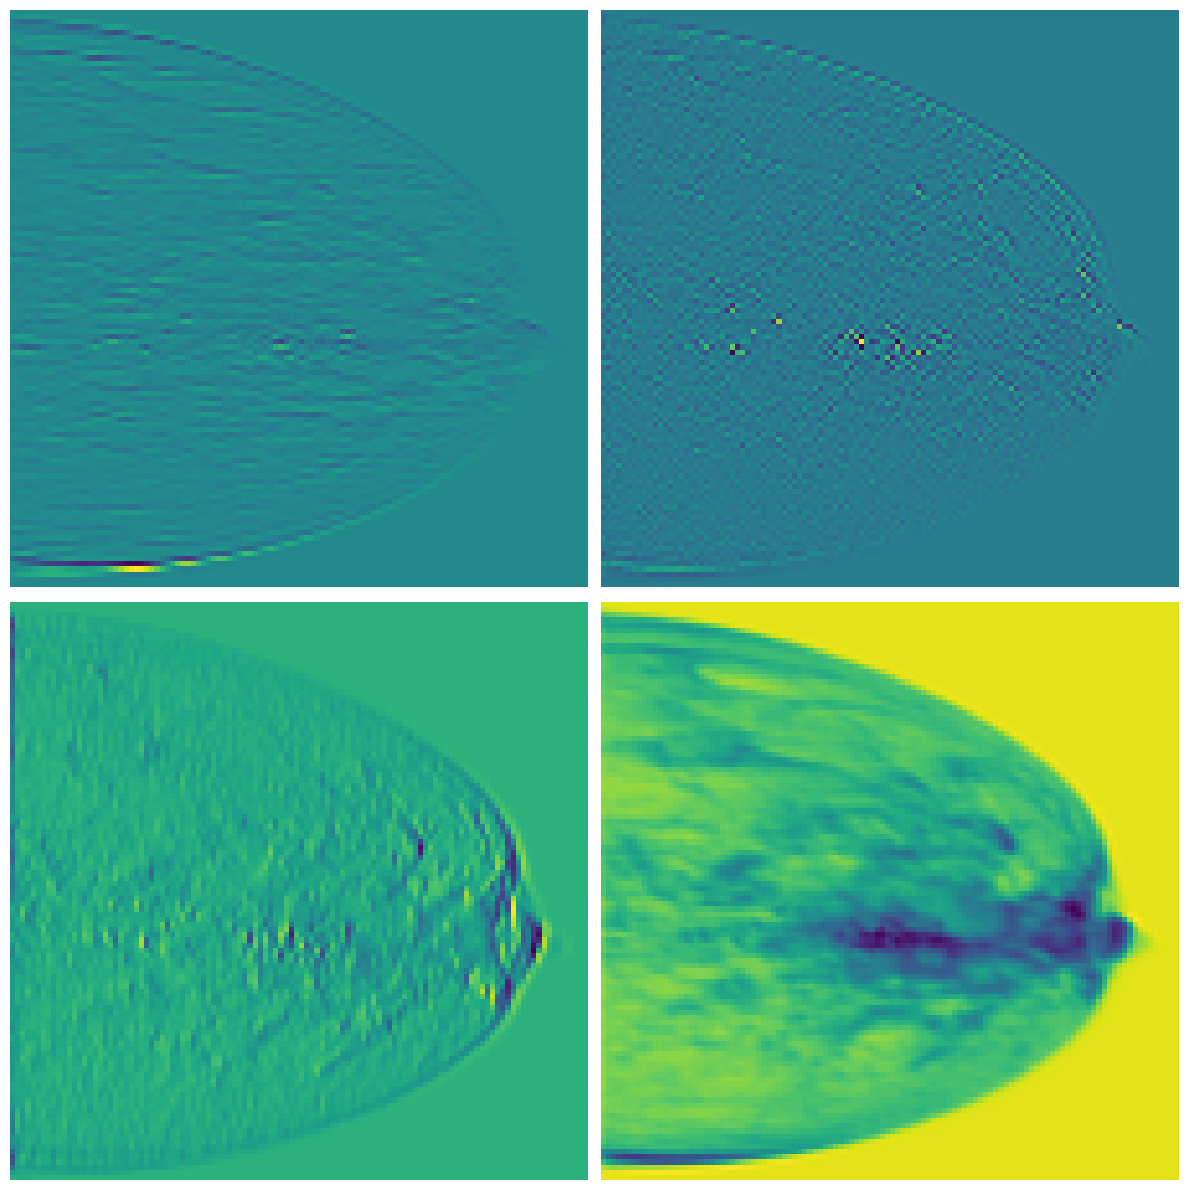
\includegraphics[width=\textwidth]{reports/assets/feature_maps_resnet.png}
            \caption{}
		\label{fig:feature_map_conv}
	\end{subfigure}
	\caption[Convolution and feature map]{(a) Illustration of the convolution operation \cite{noauthor_what_2021}. (b) Breast feature maps extracted from the first convolutional layer of Resnet101.}
\label{fig:convolution_feature_map}
\end{figure}

\textbf{Activation Functions}

Activation functions introduce non-linearity into neural networks, allowing them to learn complex patterns rather than just linear relationships \cite{langActivationFunctionsNeural2024}. They are typically applied after convolution operations to produce feature maps. Among various activation functions, the rectified linear unit (ReLU) is most commonly used in CNNs due to its simplicity, computational efficiency, and its ability to address the vanishing gradient problem \footnote{The difficulty of training deep networks caused by gradients becoming very small as they propagate through many layers.}. Popular activations functions are shown in the Figure \ref{fig:activations-functions}.

\begin{figure}
    \centering
    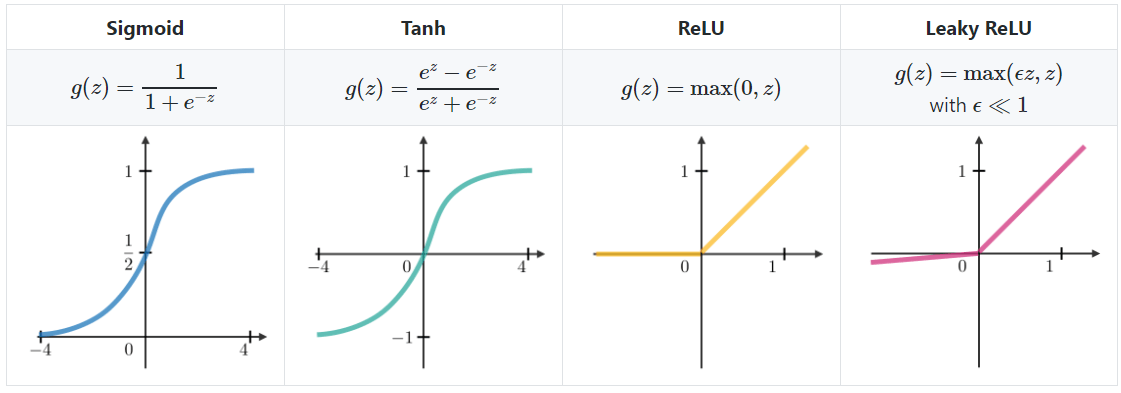
\includegraphics[width=1.0\linewidth]{reports//assets/activations_functions.png}
    \caption[Popular activation functions]{Popular activations functions used in CNN \cite{wachtelUnderstandingActivationFunctions2021}.}
    \label{fig:activations-functions}
\end{figure}

\textbf{Pooling Layers}

Pooling layers reduce the spatial dimensions of feature maps, decreasing computational complexity and helping control overfitting\footnote{A common problem in machine learning where a model learns the training data too closely, rather than capturing patterns that generalize to new, unseen data.} \cite{brownlee_gentle_2019}. Unlike convolutional layers, pooling layers perform pooling operations instead of convolutions. The most common operations are max pooling, selecting the maximum value in a region, and average pooling, computing the mean value of a region (Figure \ref{fig:pooling_operations}). Pooling is usually applied after activation functions and is often repeated throughout the network.


\begin{figure}[h!]
    \centering
    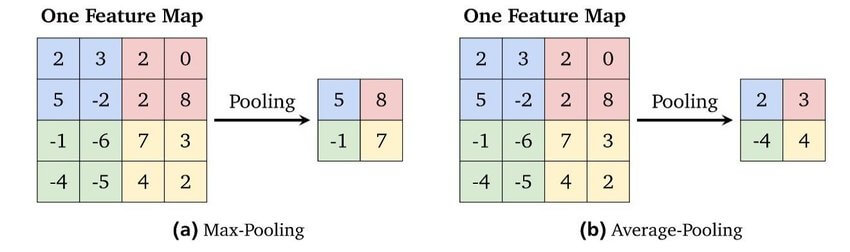
\includegraphics[width=1.0\linewidth]{reports//assets/pooling.jpg}
    \caption[Popular pooling operations]{Max pooling and Average pooling representation \cite{SkinLesionClassification}.}
    \label{fig:pooling_operations}
\end{figure}

\textbf{Fully Connected Layer}

Fully connected layers, or dense layers, are usually placed near the end of a convolutional neural network (CNN). They connect every neuron from the previous layer, consolidating features from earlier convolutional and pooling layers into a global representation. Feature maps are flattened into a one-dimensional vector before inputting into these layers, facilitating the mapping of extracted features to outputs like class probabilities \cite{noauthor_fully_nodate}. Figure \ref{fig:fc_layers} illustrates a neural network with several fully connected layers.

\begin{figure}[h!]
    \centering
    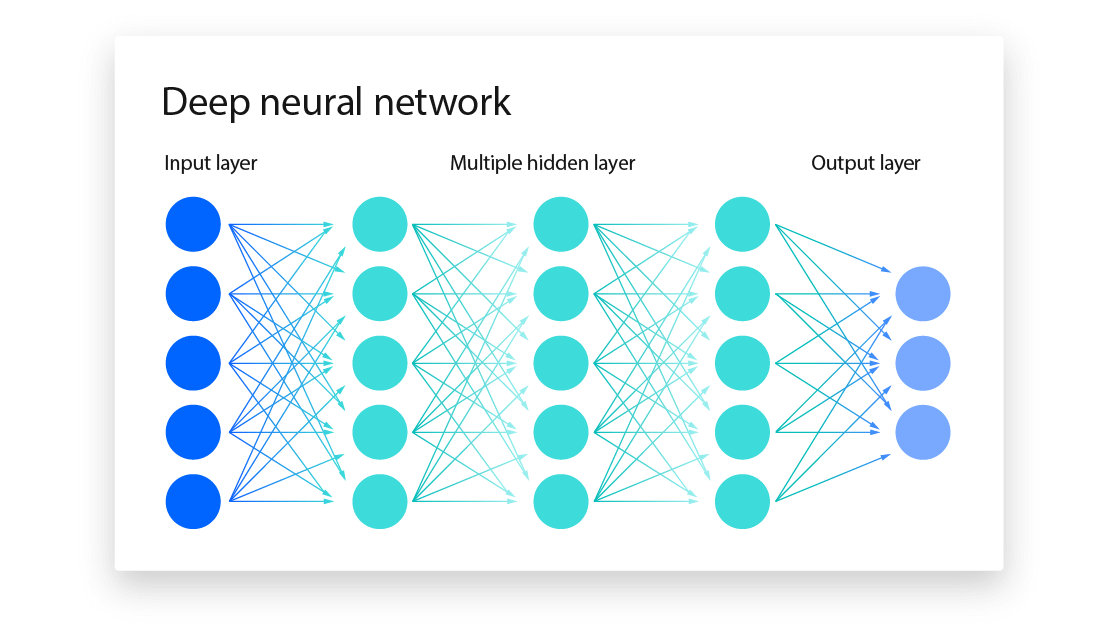
\includegraphics[width=0.75\linewidth]{reports//assets/fc_network.png}
    \caption[Fully connected layers]{Neural network with three fully connected layers and three outputs \cite{bergmann_what_2024}.}
    \label{fig:fc_layers}
\end{figure}

\textbf{Training}

With all this building blocks, CNN are constructed. Once a network is defined, it goes through the process of training, which involves the following steps \cite{bergmann_what_2024}:

\begin{enumerate}
    \item \textbf{Forward pass}: The input data passes through the network, layer by layer, to produce an output prediction.
    \item \textbf{Loss function calculation}: The difference between the predicted output and the true label is measured using a loss function.
    \item  \textbf{Backpropagation}: The network computes gradients of the loss with respect to each parameter, propagating the error backward through the layers.
    \item \textbf{Gradient descent}: The network updates its parameters (weights and biases) using the computed gradients to minimize the loss.
\end{enumerate}

After training, the network is ready to make predictions on new, unseen data. Figure \ref{fig:cnn_breast} shows an example of a complete CNN architecture for breast cancer prediction.

\begin{figure}[h!]
    \centering
    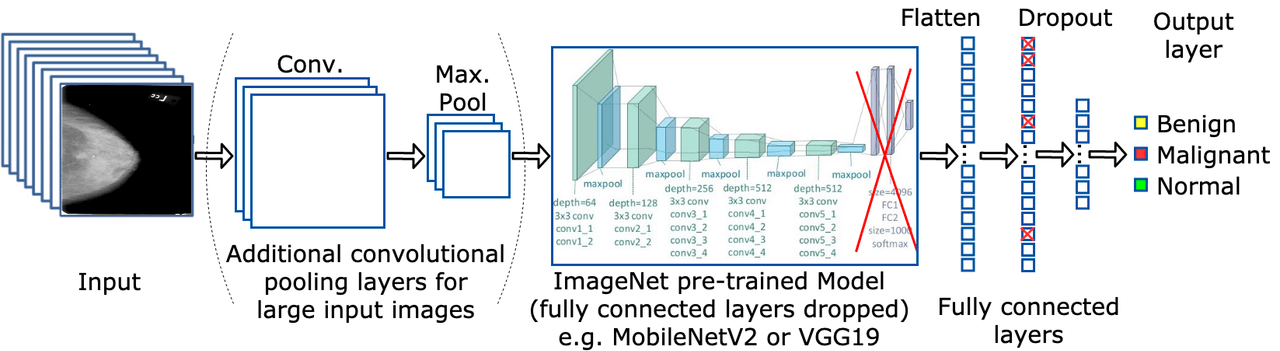
\includegraphics[width=0.9\linewidth]{reports//assets/cnn_breast.png}
    \caption[Breast cancer CNN]{CNN for breast cancer prediction \cite{jaamour_divide_2023}.}
    \label{fig:cnn_breast}
\end{figure}

\subsection{Main Architectures}

\textbf{VGGNet (VGG16/VGG19)}

Symonyan et al. (2015) introduced VGGNets \cite{simonyanVeryDeepConvolutional}. Renowned for their straightforward design and depth, they employ solely 3×3 convolutions and can have up to 19 layers. They are extensively utilized as feature extractors and serve as a fundamental benchmark for transfer learning in both medical and general image applications.

\textbf{ResNet}

He et al. (2015) \cite{he_deep_2015} presented Residual Networks, or ResNets, as a solution for training very deep neural networks with over 50 layers, which helps address the problem of vanishing gradients. This is achieved through the implementation of residual or skip connections between layers. ResNet is the default choice for many image analysis tasks due to its robustness and ease of training.

As previously stated, this study uses ResNet-101 as the baseline model. This architecture, comprised of 101 layers with residual connections, proves highly performance at managing complex tasks. Figure \ref{fig:resnet_101} illustrate an overview of its structure.

\begin{figure}[h!]
    \centering
    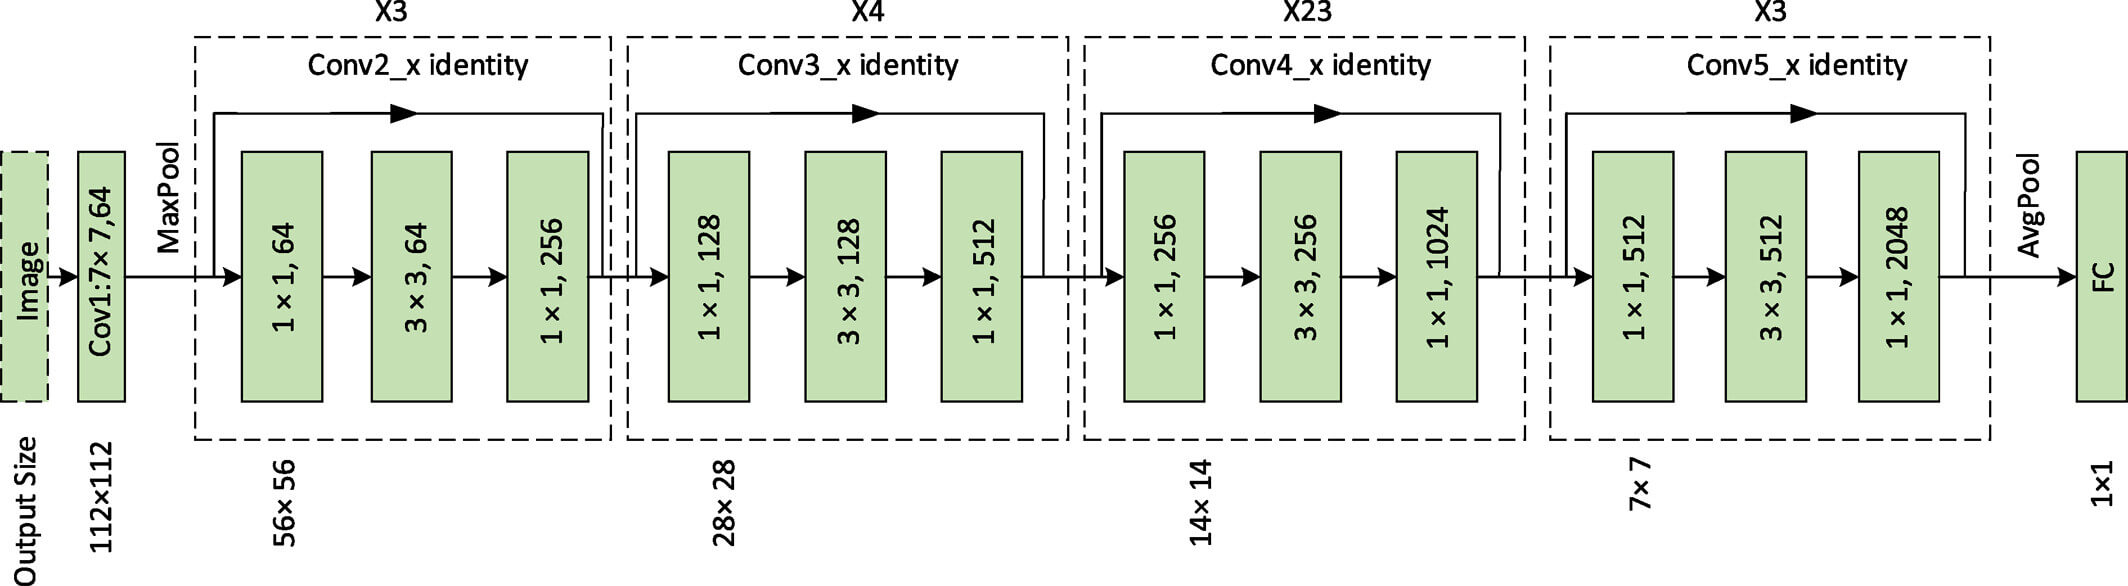
\includegraphics[width=0.75\linewidth]{reports//assets/resnet101.jpg}
    \caption[ResNet-101 Architecture]{ResNet-101 Architecture.}
    \label{fig:resnet_101}
\end{figure}


\subsection{CNNs Limitations}

CNNs offer numerous advantages and a wide range of applications; however, they also have certain limitations that deserve consideration:

\begin{itemize}
    \item \textbf{Limited global context}: CNN mainly capture local features and struggle with global context, which is important in medical imaging.
    
    \item \textbf{Rigid inductive bias}: Their design enforces assumptions like locality and translation invariance, limiting flexibility for learning more abstract or non-local patterns.
    
    \item \textbf{Generalization across diverse data}: CNNs often have difficulty generalizing to data from different sources or patient populations, reducing their robustness in clinical settings.
\end{itemize}

Recent advances in Transformer-based models offer promising solutions to some of these limitations by enabling better modeling of global context and improving generalization, which will be discussed in the following section.

\section{Transformer-Based models}

Transformer models are built upon the Transformer architecture, which was initially developed for natural language processing (NLP) tasks. Since their introduction to computer vision, these models have gained significant popularity as an alternative to CNNs due to their effectiveness in capturing global context and modeling long-range dependencies within images \cite{pereira_review_2024}. 

In this section, we review what transformer-based models are and describe the architectural designs of those analyzed in this work for the task of breast cancer molecular subtype classification.

\subsection{The Transformer architecture}

The Transformer architecture is a DL model introduced by Vaswani et al. (2017) in their seminal paper “Attention is All You Need” \cite{vaswani_attention_2017}. Originally developed as an alternative to recurrent neural networks (RNNs)\footnote{A special class of artificial neural network designed to process sequential or time-series data, such as text, speech, or sensor readings.} for sequence-to-sequence tasks in NLP, the Transformer has since become widely adopted in computer vision as well.

At its core, the Transformer consists of an encoder-decoder structure built from repeated layers containing two key components: multi-head self-attention and position-wise feed-forward networks (see Figure~\ref{fig:transformer}). This design enables the model to capture both local and global dependencies by relating every element in the input sequence to every other element, regardless of their positions.

\begin{figure}[h!]
    \centering
    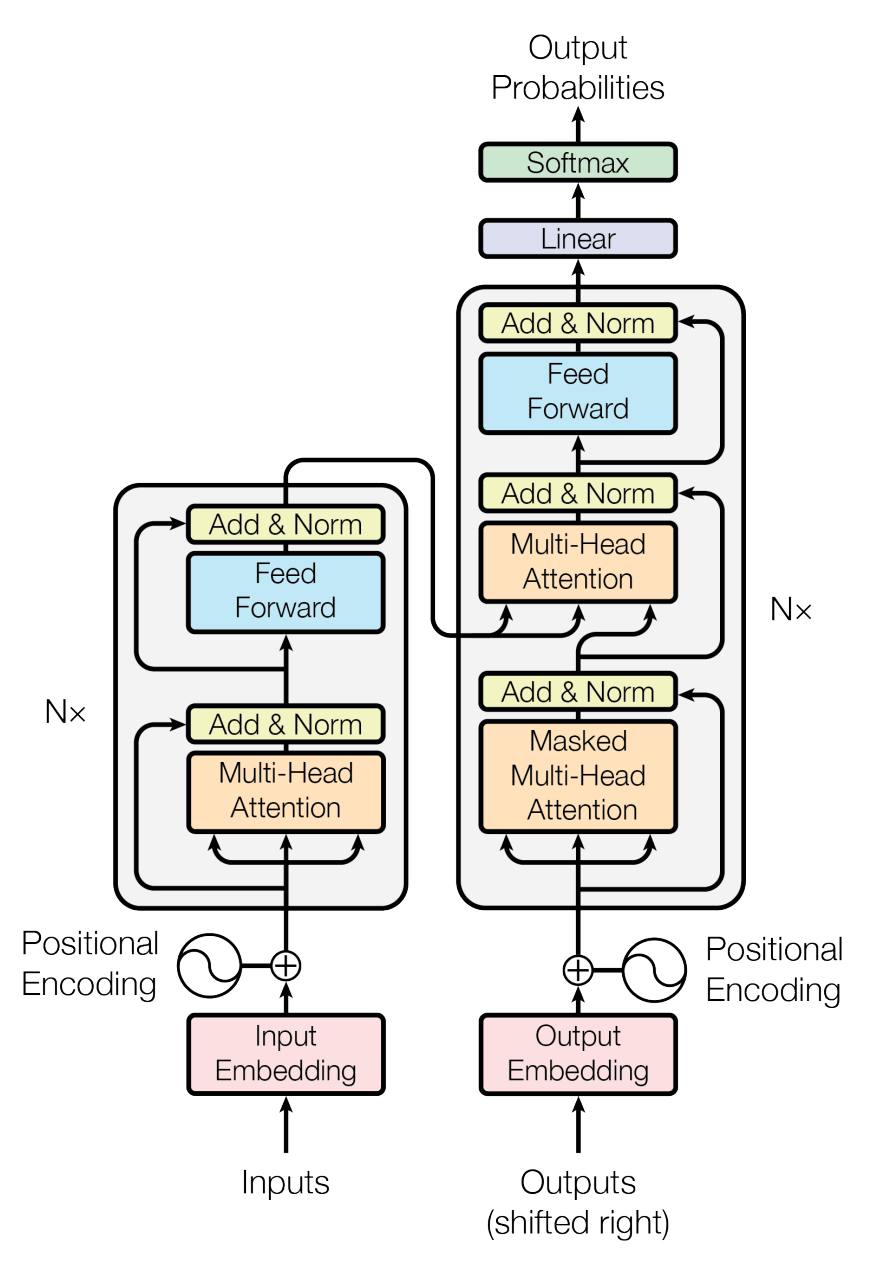
\includegraphics[width=0.5\linewidth]{reports//assets/transformer.png}
    \caption[Transformer Architecture]{The Transformer Architecture \cite{vaswani_attention_2017}.}
    \label{fig:transformer}
\end{figure}

\textbf{Self-Attention}

Self-attention is an attention mechanism\footnote{A technique in machine learning that enables models to focus on the most relevant parts of the input data when making predictions or generating outputs.} that allows a network to relate different positions within a single input sequence, thereby computing a context-aware representation for each element. In simpler terms, it enables the model to efficiently prioritize and integrate important information from across the entire input. The concept of attention was first introduced by Bahdanau et al. (2014) \cite{bahdanau_neural_2014}, but it was the Transformer architecture that first relied entirely on self-attention to compute representations \cite{vaswani_attention_2017}. In a concise overview, this process functions as follows:

\begin{itemize}
    \item \textbf{Projection}: Each input element is projected into three distinct vectors:
        \begin{itemize}
        \item \textbf{Query (Q)}: Represents the current element (e.g., a word or image patch) for which we want to find relevant information from the sequence.
        \item \textbf{Key (K)}: Represents each element in the sequence and is used to match against queries to measure their relevance.
        \item \textbf{Value (V)}: Contains the actual information of each element, which will be combined according to the attention scores.
        \end{itemize}
    \item \textbf{Score Calculation}: For each element, an attention score is computed by taking the dot product between its query and all keys in the sequence.
    \item \textbf{Scaling}: Each score is divided by the square root of the key dimension to stabilize training and prevent large gradients.
    \item \textbf{Softmax Normalization}: The softmax\footnote{The softmax function transforms the scores into probabilities that sum to one.} function is applied to the scaled scores to obtain attention weights.
    \item \textbf{Weighted Sum}: A new, context-aware representation for each input element is obtained by computing the weighted sum of all value vectors using the attention weights.
\end{itemize}

Figure \ref{fig:scaled_dot_product_attn} illustrates the process of scaled dot-product attention in detail. Mathematically, the process can be summarized as follows:

$$Attention(Q,K,V) = softmax\left(\frac{QK^T}{\sqrt{d_k}}\right)V$$

\begin{figure}[h!]
    \centering
    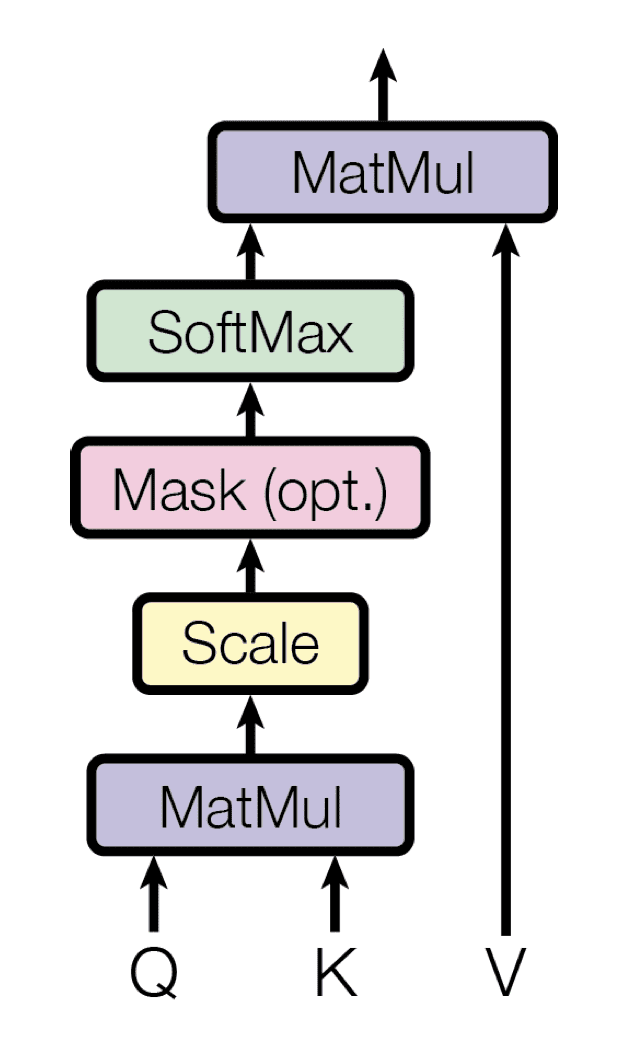
\includegraphics[width=0.3\linewidth]{reports//assets/scaled_dot_product.png}
    \caption[Scaled dot-product attention]{Scaled dot-product attention mechanism \cite{vaswani_attention_2017}.}
    \label{fig:scaled_dot_product_attn}
\end{figure}


\subsection{Vision Transformer}

A Vision Transformer (ViT) is a DL  architecture introduce by Dosovitskiy et al. (2020) \cite{dosovitskiy_image_2020} designed for computer vision tasks, inspired by the Transformer architecture originally developed for NLP. 

\textbf{ViT processing pipeline}

A ViT processes an image by first dividing it into fixed-size patches, for example, a 224×224 image split into 16×16 patches results in 196 patches. Each patch is then flattened and projected into an embedding space by the patch embedding layer. Because the ViT architecture lacks inherent spatial awareness, positional encodings are added to each patch embedding to preserve spatial information within the image. This design allows the input to be treated analogously to a sequence of tokens in NLP Transformers. As the sequence passes through multiple layers of multi-head self-attention, the model learns to capture both local and global relationships among the patches, enabling robust image understanding. This process and the ViT architecture is depicted in the Figure \ref{fig:vit_arch}.


\begin{figure}[h!]
    \centering
    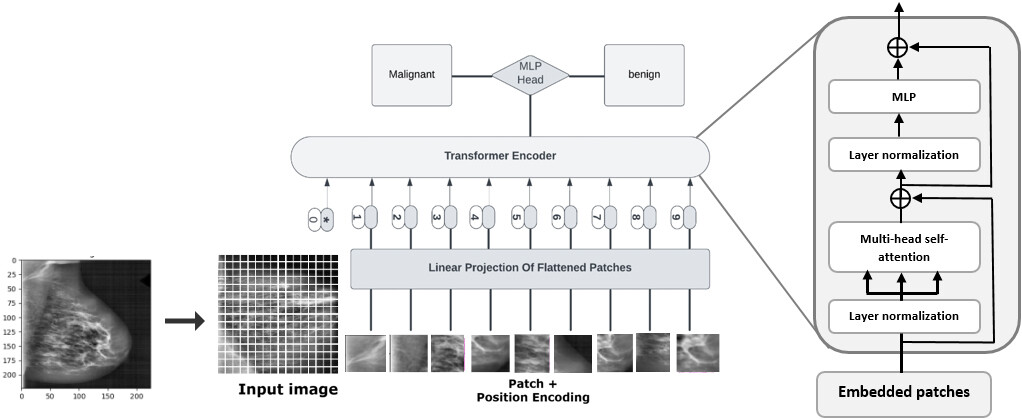
\includegraphics[width=1.0\linewidth]{reports//assets/vit_breast.jpg}
    \caption[Vision Transformer Architecture]{ViT architecture, in this example, for breast cancer classification \cite{abimouloud_vision_2024}.}
    \label{fig:vit_arch}
\end{figure}

ViTs have rapidly expanded their reach to many computer vision tasks, including image classification, object detection, and image segmentation. In medical imaging, several studies have evaluated their performance on tasks such as breast cancer classification, consistently reporting strong results \cite{marquez_vara_vision_2024, mauricio_comparing_2023, ayana_vision-transformer-based_2023}.


\subsection{Shifted-Window Transformer}

Shifted-Window Transformers (Swin), introduced by Liu et al. (2021) \cite{liu_swin_2021}, are a specialized architecture derived from Vision Transformers (ViT). They are designed to address some of the limitations of ViT, particularly regarding computational efficiency and scalability when processing high-resolution images.

To achieve this, Swin employs a shifted window mechanism. Unlike ViT, which typically applies self-attention globally, Swin divides the image into a set of non-overlapping windows (Figure \ref{fig:swin_vit}), with each window containing a subset of image patches. Self-attention is then applied locally within each window, significantly reducing computational complexity. The windows are shifted between layers to enable cross-window connections and enhance information flow across the entire image.

\begin{figure}[h!]
    \centering
    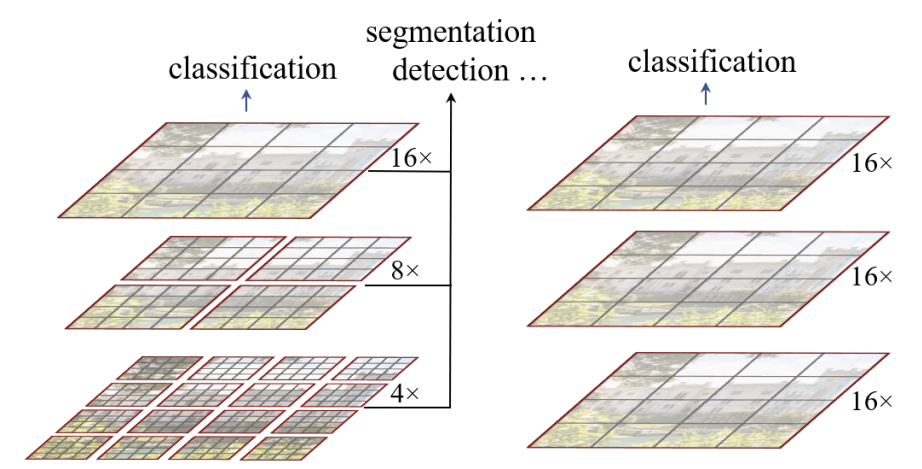
\includegraphics[width=0.6\linewidth]{reports//assets/Swin.png}
    \caption[Comparison of Swin and ViT mechanisms]{Comparison of Swin and ViT attention mechanisms. \textbf{Left:} Swin Transformer with shifted window self-attention. \textbf{Right:} Vision Transformer (ViT) with global self-attention across all patches \cite{liu_swin_2021}.}
    \label{fig:swin_vit}
\end{figure}

As a result of this mechanism, Swin exhibits a computational complexity of $O(n)$, whereas ViT has a complexity of $O(N^2)$. 



\begin{figure}[h!]
    \centering
    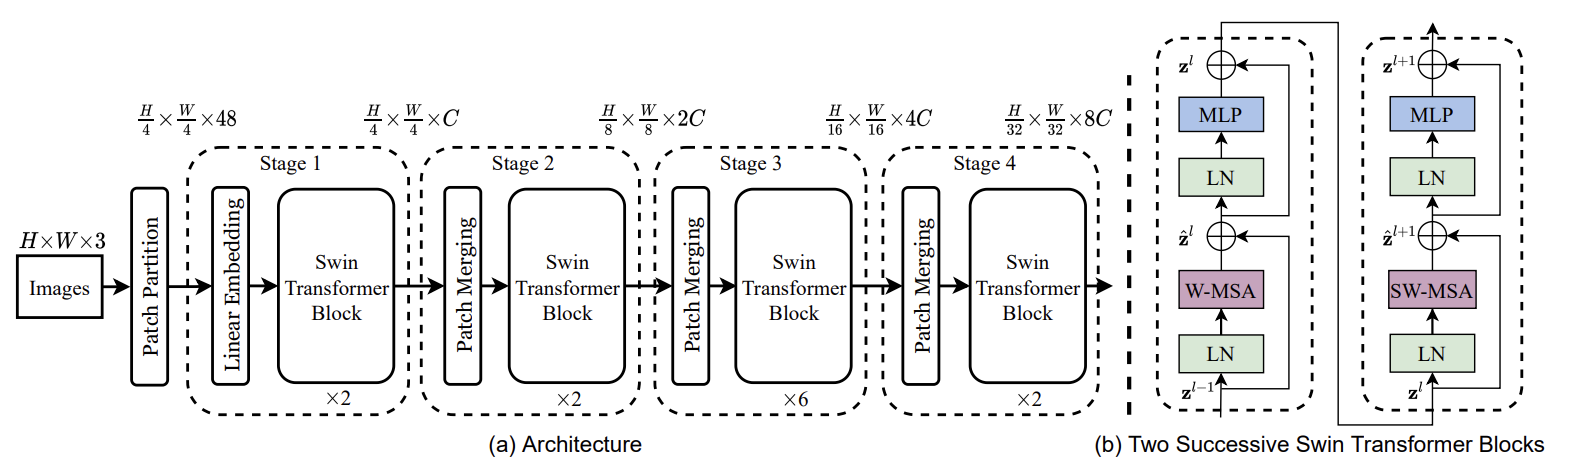
\includegraphics[width=1.0\linewidth]{reports//assets/SwinArch.png}
    \caption[Swin Transformer Arch]{Swin Transformer Architecture \cite{liu_swin_2021}.}
    \label{fig:swin_arch}
\end{figure}

\subsection{Multi-Axis Vision Transformer}

Multi-Axis Vision Transformer (MaxViT) is a hybrid vision transformer architecture introduced by Tu et al. (2022) \cite{tu_maxvit_2022}. It is designed to capture both local and global spatial relationships in images, overcoming scalability and capacity limitations of previous transformer-based models. MaxViT achieves this by combining blocked local attention (as in Swin, but without shifting) and dilated global (grid) attention within each block, together with convolutional layers. This multi-axis attention mechanism allows MaxViT to efficiently model both short- and long-range dependencies while maintaining the same linear computational complexity as Swin. Figure \ref{fig:max_vit_arch} illustrates this structure.

\begin{figure}[h!]
    \centering
    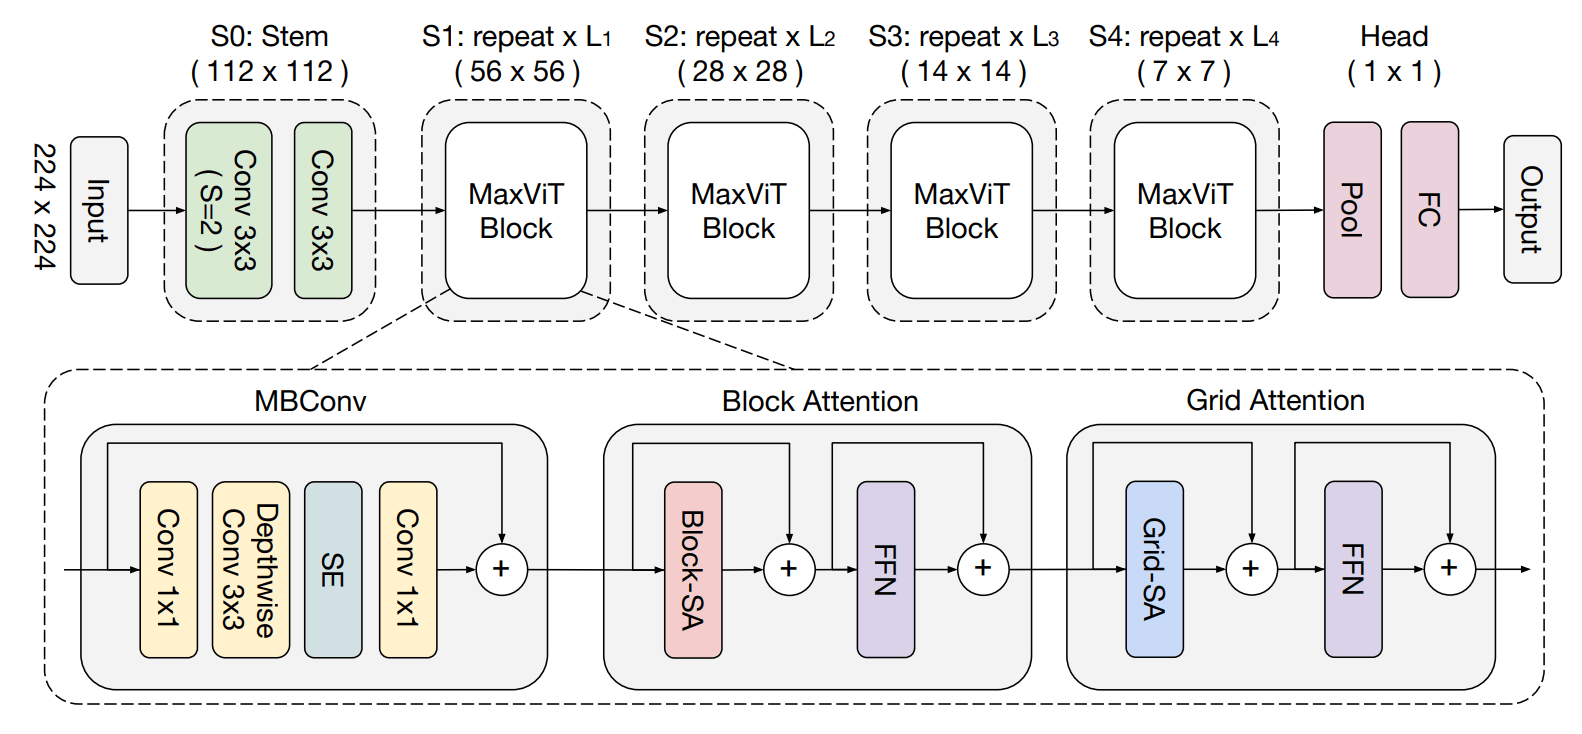
\includegraphics[width=1.0\linewidth]{reports//assets/maxvit_arch.png}
    \caption[Multi-Axis Vision Transformer Arch]{MaxVit Architecture \cite{tu_maxvit_2022}.}
    \label{fig:max_vit_arch}
\end{figure}


\textbf{Multi-Axis Attention}

Multi-axis attention is the key component of MaxViT. It works by splitting the attention mechanism into two parts: a block of local attention, which focuses on local regions (similar to Swin’s), and a grid attention block, which enables global information flow across the entire image through a dilated, grid-like pattern. This design allows MaxViT to efficiently capture both local and global dependencies within each block (see Figure \ref{fig:multi_axis_attention}).

\begin{figure}[h!]
    \centering
    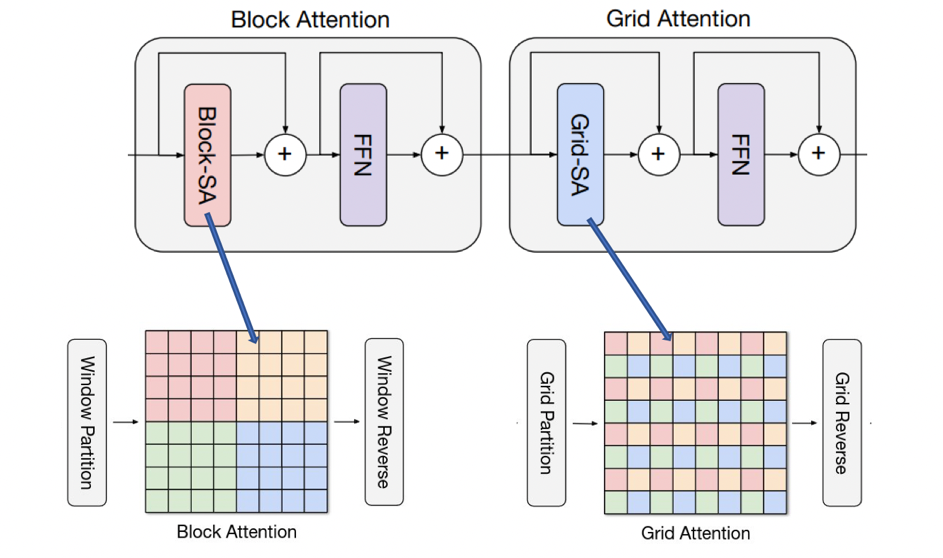
\includegraphics[width=0.6\linewidth]{reports//assets/multi_axis_attention.png}
    \caption[Multi-Axis Attention Blocks]{Multi-Axis attention blocks \cite{noauthor_maxvit-unet_2024}.}
    \label{fig:multi_axis_attention}
\end{figure}


\section{Training and Evaluation Techniques}
\subsection{Transfer Learning}

Transfer learning is a ML technique in which a model developed and trained on one task or dataset is reused or fine-tuned to improve performance on a different, but related, task. It is especially valuable when data is limited or the target task has few labeled examples available \cite{murel_what_2024}. In other words, instead of training a new model from scratch, transfer learning leverages knowledge previously obtained, such as learned features and weights, often from large datasets, to accelerate and enhance learning on a new problem.

This approach is very popular and widely used to avoid training new machine learning or deep learning models from scratch. In medical imaging, for example, where annotated data is often scarce or expensive to obtain, transfer learning has enabled the development and training of models that reduce training time, improve performance, and promote feature reuse \cite{matsoukas_what_2022}. This process is depicted in Figure \ref{fig:transfer_learning}.

\begin{figure}[h!]
    \centering
    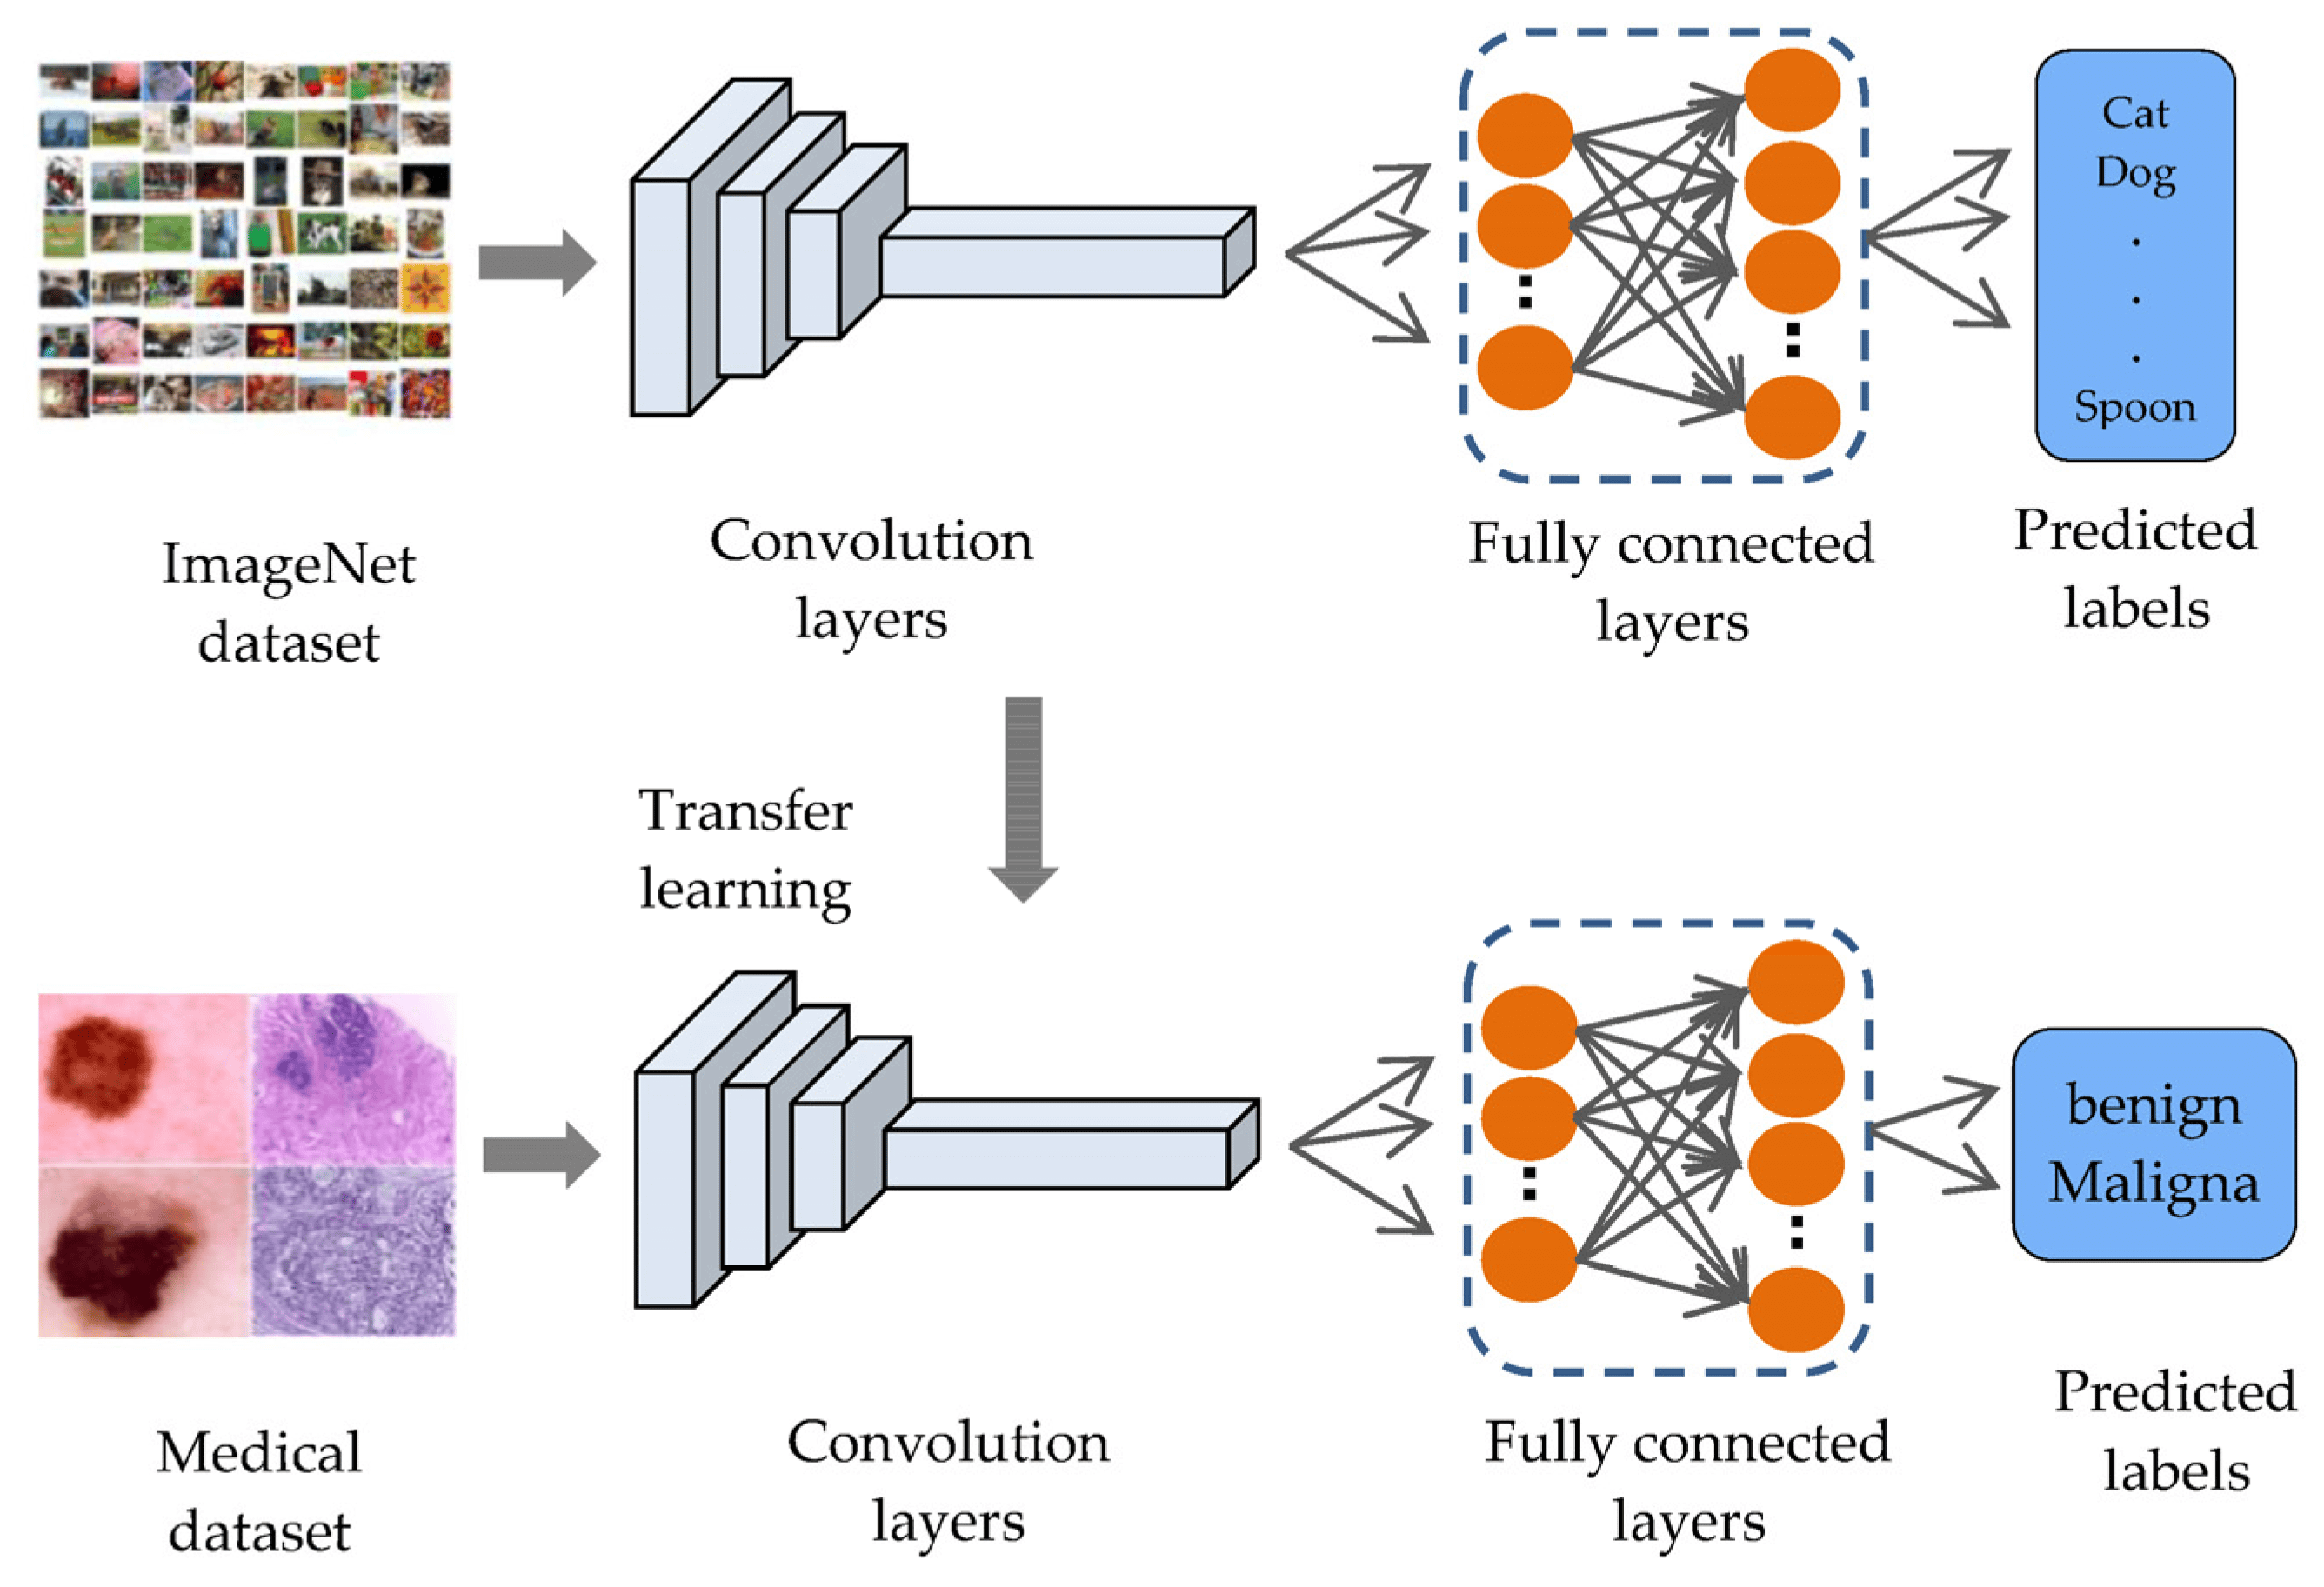
\includegraphics[width=0.75\linewidth]{reports//assets/transfer-learning.png}
    \caption[Transfer learning process]{Transfer learning process where}
    \label{fig:transfer_learning}
\end{figure}


\subsection{Fine-Tuning}

Fine-tuning is a specific technique within transfer learning that involves taking a pre-trained model and continuing its training on a smaller or more specialized dataset to adapt its capabilities to a particular case or domain \cite{noauthor_what_2024}. During fine-tuning, some or all of the model’s parameters are unfrozen and updated, allowing the model to learn features relevant to the new task while retaining the general knowledge acquired during pre-training. However, training large models on small datasets can lead to overfitting, so it is common practice to use a lower learning rate during fine-tuning to make gradual adjustments and preserve previously learned representations.

\subsection{K-Fold Cross-Validation}

K-Fold Cross-Validation is a robust evaluation technique used in machine learning when data is limited or a single train/test split may not provide reliable results. The dataset is divided into $K$ equal parts, or folds. The model is then trained and validated $K$ times, each time using a different fold as the validation set and the remaining folds for training. This process ensures that every sample is used for both training and validation, leading to a more reliable and less biased estimate of model performance. By averaging results across all folds, K-Fold Cross-Validation reduces variance and is especially useful for small or imbalanced datasets. Figure \ref{fig:k_fold} illustrates this process.

\begin{figure}[h!]
    \centering
    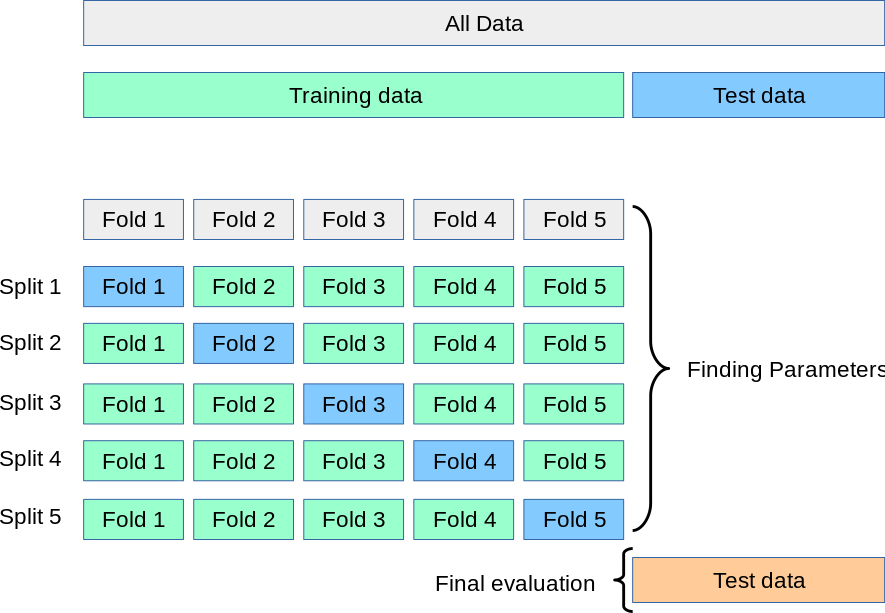
\includegraphics[width=0.75\linewidth]{reports//assets/k-fold.png}
    \caption[K-Fold Cross Validation]{K-Fold cross validation process, in this example, $K$ = 5 \cite{noauthor_31_nodate}.}
    \label{fig:k_fold}
\end{figure}

\subsection{AI Explainability}

DL models, while highly effective in medical image analysis, are often criticized for their lack of interpretability—commonly referred to as the “black box”\footnote{Refers to a system where the internal workings are opaque and not easily understandable, even by the creators.} problem. Explainability techniques aim to address this challenge by providing visual or quantitative insights into the decision-making process of these models. In the context of breast cancer detection and molecular subtyping from mammographic images, model transparency is especially important for building clinical trust and aiding radiologists in understanding AI-driven predictions. Two state-of-the-art explainability methods are presented: Grad-CAM, designed for convolutional neural networks, and ViT-ReciproCAM, tailored for Vision Transformers.

\textbf{Grad-CAM}

Grad-CAM (Gradient-weighted Class Activation Mapping) is an explainability technique for CNNs that creates visual explanations by highlighting key regions in input images that significantly influence a model's prediction \cite{noauthor_161002391_nodate}. It computes gradients of the target class score relative to the feature maps of a selected convolutional layer to generate a class-specific localization map. This technique aids in interpreting image regions contributing to model decisions, especially useful in medical imaging where model transparency is critical.

\textbf{ViT-ReciproCAM}

ViT-ReciproCAM is a recent explainability method specifically designed for Vision Transformers (ViTs). Unlike traditional techniques such as Grad-CAM, which rely on gradient and attention information, ViT-ReciproCAM is gradient and attention-free \cite{byun_vit-reciprocam_2023}. It operates by masking tokens in the feature map from the last transformer encoder block and measuring the effect of these masks on the model’s output. This process exploits the correlation between masked tokens and the network’s predictions for a given class, producing localized saliency maps that indicate the most influential image regions.

\begin{figure}
    \centering
    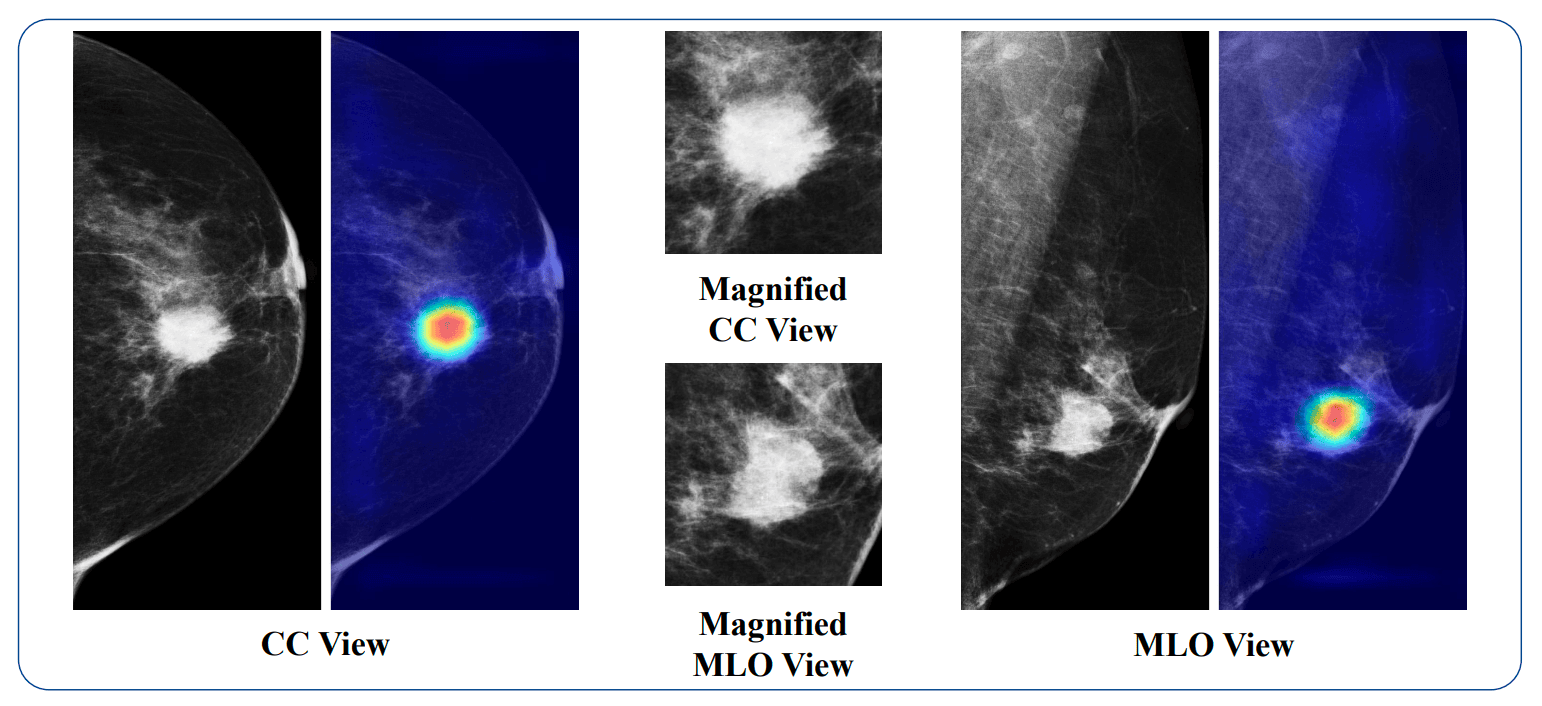
\includegraphics[width=0.8\linewidth]{reports//assets/grad-cam.png}
    \caption[Grad-CAM example]{Example of the Grad-CAM technique applied to a mammogram, highlighting the region corresponding to the mass \cite{panambur_classification_2023}.}
    \label{fig:grad-cam-example}
\end{figure}

\chapter{Materials and Methods}

This section outlines the materials and methods utilized in this study. It begins with a description of the dataset chosen for model training and analysis, then discusses the processing and preparation of the images, and concludes with the evaluation metrics for assessing model performance.


\section{The Chinese Mammography Database}

The Chinese Mammography Database (CMMD) is a public dataset developed by Cai et al. (2023) \cite{cai_online_2023} and hosted on The Cancer Imaging Archive (TCIA)\footnote{\url{https://www.cancerimagingarchive.net/collection/cmmd/}}. This dataset includes a total of 3,712 mammograms from 1,775 Chinese patients, in CC and MLO views, collected between July 2012 and January 2016. CMMD is divided into two subsets:

\begin{itemize}
    \item \textbf{CMMD1}: This subset includes samples with both malignant and benign diagnoses, along with key clinical data such as patient age, type of abnormality, and tumor classification.
    \item \textbf{CMMD2}: This subset contains only malignant diagnoses, providing the same metadata as CMMD1, but with the addition of molecular subtype classification for each tumor.
\end{itemize}


Table \ref{tab:cmmd_features} shows the main features detailed of each subset.

\begin{table}
	\caption[CMMD subsets features]{Main features of the CMMD subsets}
	\centering
	\begin{tabular}{lccccc}
		\toprule
		                                 & \textbf{CMMD1}       & \textbf{CMMD2}      &      \\
		\midrule
		\textbf{Number of patients}      & 1026                 & 749                 & 1775 \\
		\textbf{Number of mammographies} & 2230                 & 1498                & 3728 \\
		\textbf{Mean patient age}        & 45.92 (17-84 years)  & 49.82 (21-87 years) & -    \\
		\textbf{Diagnosis outcome}       & Benign and Malignant & Malignant           & -    \\
		\textbf{Molecular subtype}       & No                   & Yes                 & -    \\
		\bottomrule
	\end{tabular}
	\label{tab:cmmd_features}
\end{table}

\subsection{CMMD2 Subset Selection}

In this research, the focus is exclusively on the CMMD2 subset, as it is the only publicly available and of free access dataset that provides molecular subtype annotations. These annotations are essential for training models in breast cancer molecular subtype classification, which is the primary objective of this study.

\subsection{CMMD2 General Description}

For the composition of CMMD2, only cases with complete immunohistochemical marker information and a confirmed diagnosis of invasive carcinoma were selected, as detailed in the inclusion and exclusion criteria shown in Figure~\ref{fig:cmmd_criteria}. Applying these criteria resulted in a subset comprising 1,498 mammographies from 749 patients. Since each patient has both CC and MLO views, the total number of images is 2,996 for this subset.

\begin{figure}[h!]
	\centering
	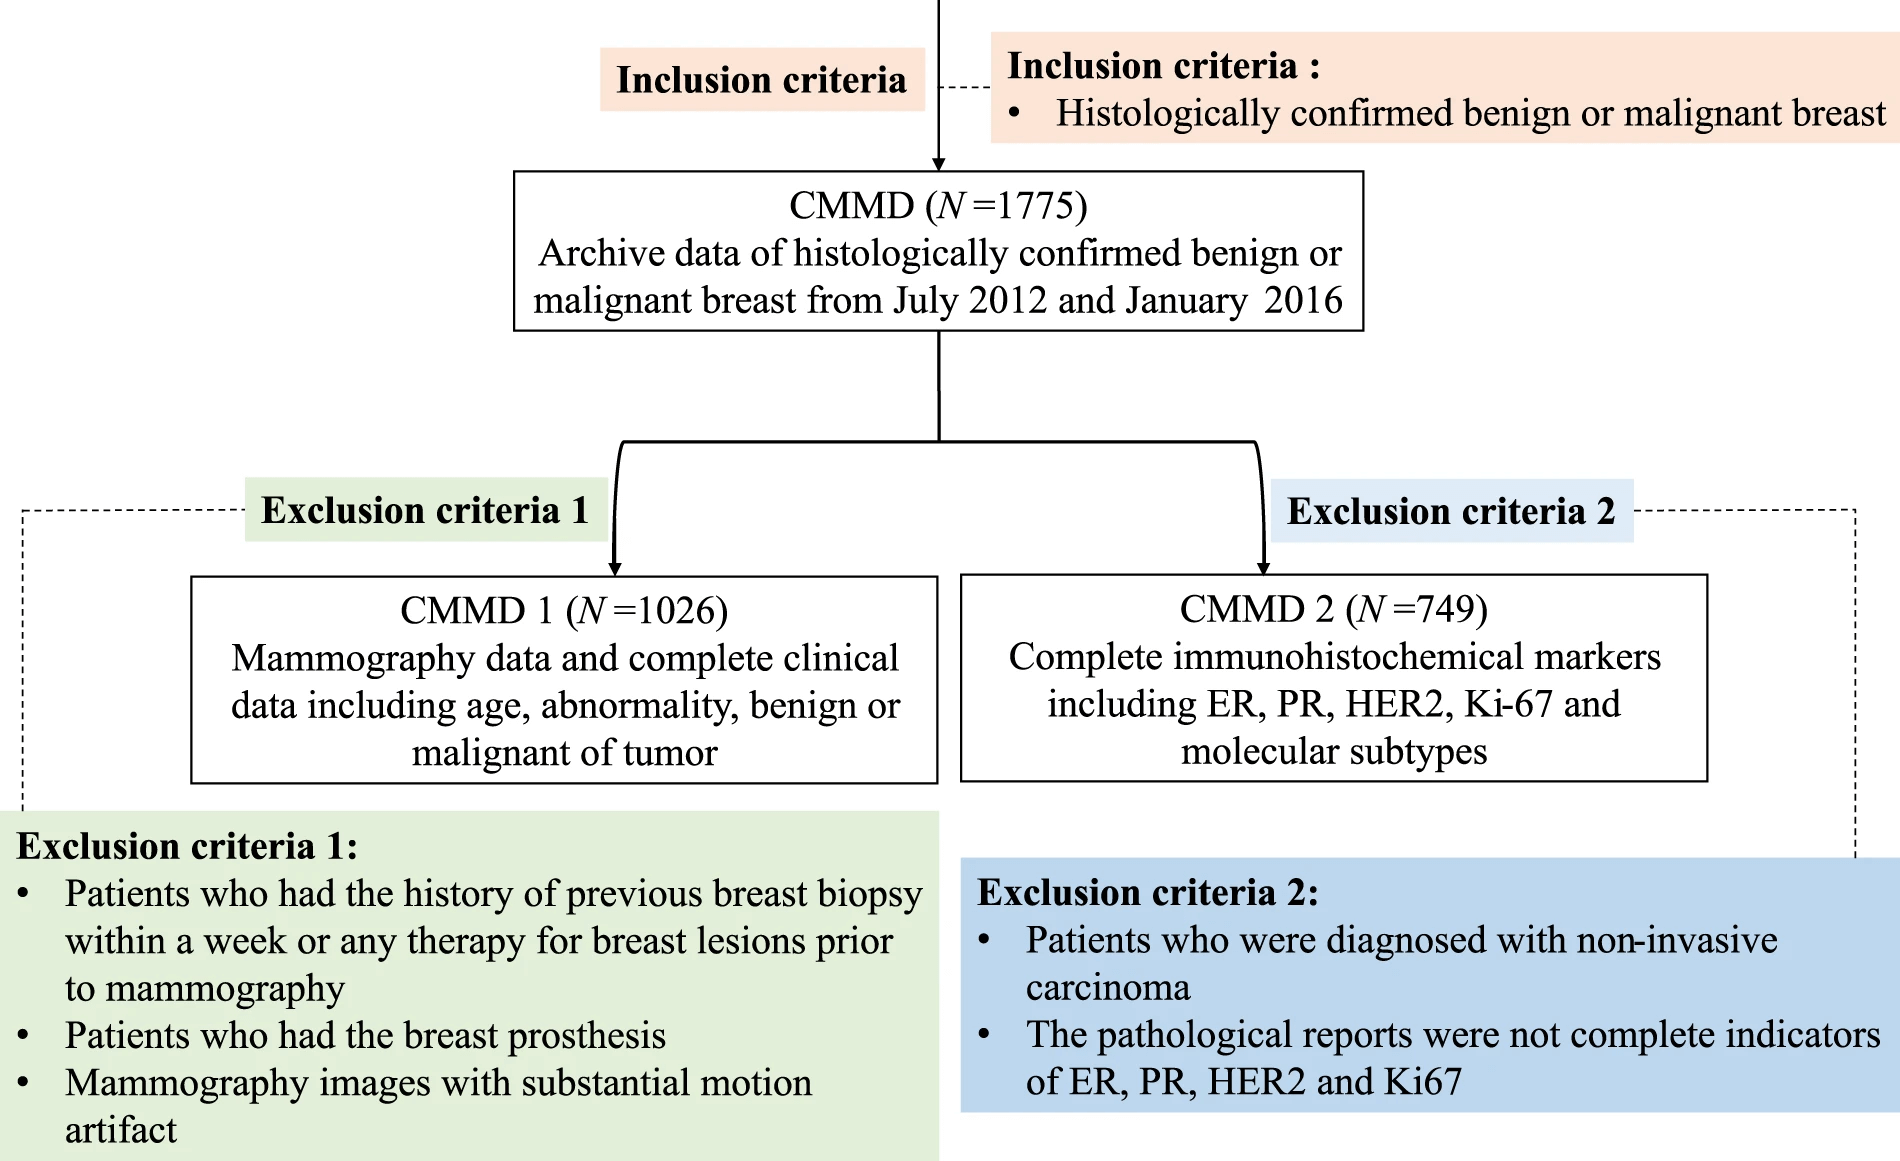
\includegraphics[width=0.85\linewidth]{reports//assets/cmmd_criteria.png}
	\caption[CMMD's inclusion and exclusion criteria]{CMMD's inclusion and exclusion criteria \cite{cai_online_2023}.}
	\label{fig:cmmd_criteria}
\end{figure}

\textbf{Image Collection}

The mammography images were collected using the \textbf{GE Senographe DS} mammography system, obtaining both CC and MLO views for each patient. The images were then stored in 8-bit grayscale at a image size of 2294×1914 pixels \cite{cai_online_2023}.

\textbf{Image Format and Resolution}

The main format of the images in the dataset is DICOM (Digital Imaging and Communications in Medicine), the standard in medical imaging, as it allows clinical metadata to be stored alongside the image and enables interoperability between equipment from different manufacturers as well as interaction between different information systems in hospitals and healthcare centers.

\subsection{CMMD2 Metadata}

For each patient, the dataset provides a CSV\footnote{A plain text file that stores data in tabular form, where each line represents a row and each value in the row is separated by a comma} (Comma Separated Values) file with additional information to the obtained images, including age, laterality, type of abnormality, classification, and in the case of CMMD2, also the molecular subtype of the tumor. Table \ref{tab:cmmd2_metadata} describes these data in detail.

\begin{table}[h!]
	\caption[CMMD2 metadata description]{Description of metadata variables present in the CMMD2 dataset.}
	\centering
	\begin{tabular}{>{\bfseries}l p{5cm} p{6cm}}
		\toprule
		\textbf{Column} & \textbf{Description}                 & \textbf{Possible values}                             \\
		\midrule
		ID1             & Unique patient identifier            & Format: D2-XXXX                                      \\
		LeftRight       & Breast laterality                    & L (left), R (right)                                  \\
		Age             & Patient age at the time of the study & Between 21 and 87 years                              \\
		Number          & Number of images available per study & Between 2 and 4                                      \\
		Abnormality     & Type of abnormality                  & Mass, Calcification, Both                            \\
		Classification  & Nature of the abnormality            & Benign, Malignant                                    \\
		Subtype         & Molecular subtype of breast cancer   & Luminal A, Luminal B, HER2-enriched, Triple negative \\
		\bottomrule
	\end{tabular}

	\label{tab:cmmd2_metadata}
\end{table}

It is important to note that, the laterality column indicates the side where the tumor was found; therefore, the opposite side is considered benign \cite{cai_online_2023}.

The age distribution of patients follows an approximately normal distribution with slight asymmetries. The most frequent age range is between 45 and 55 years, which is consistent with breast cancer epidemiology, where the majority of cases are diagnosed during this age interval. The inclusion of younger patients in the dataset enhances population diversity and enables analysis of model performance across underrepresented demographic subgroups. Figure \ref{fig:age_dist_all} illustrates this distribution.


\begin{figure}[h!]
	\centering
	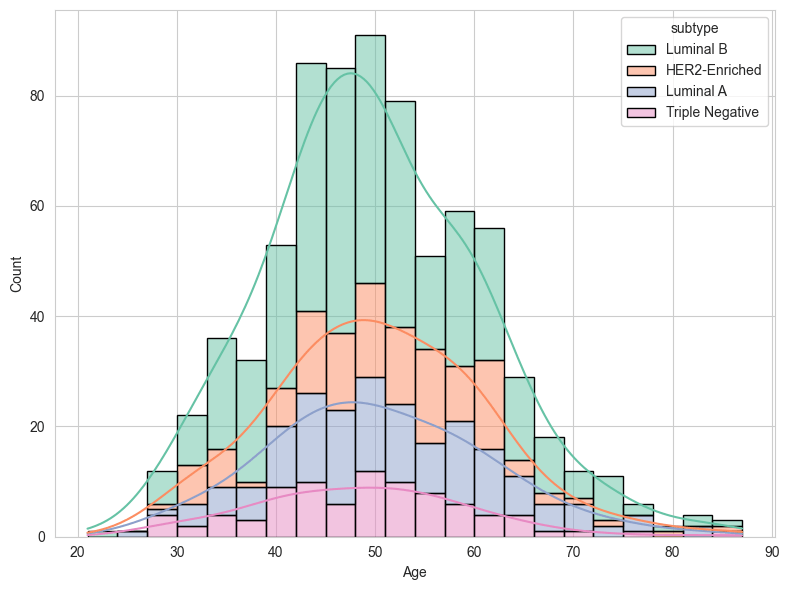
\includegraphics[width=0.5\linewidth]{reports//assets/age_dist.png}
	\caption[CMMD2 Age distribution]{CMMD2 Overall age distribution of patients and molecular subtype.}
	\label{fig:age_dist_all}
\end{figure}

The analysis of molecular subtype distribution within the CMMD2 dataset is also crucial, as it determines the statistical representativeness of each class and consequently affects the models' generalization capability in clinical scenarios. The dataset exhibits significant class imbalance\footnote{Class imbalance refers to unequal representation of different classes in a dataset, where some classes have substantially more or fewer samples than others.}, with Luminal B being the most prevalent subtype (376 patients, 50.2\%), followed by Luminal A (152 patients, 20.3\%), HER2-enriched (135 patients, 18.0\%), and Triple Negative as the least represented subtype (86 patients, 11.5\%).

The class imbalance is also reflected in the total number of images available per subtype, as each patient contributes at least two mammographic views (CC and MLO projections), with few exceptions. This imbalance presents a significant challenge for machine learning classification models, which tend to exhibit bias toward majority classes when appropriate balancing strategies are not implemented. Nevertheless, this distribution accurately reflects the relative prevalence observed in clinical practice, where Luminal subtypes (A and B) are most common, while Triple Negative breast cancer represents approximately 10-15\% of all cases.

\begin{figure}[h!]
	\centering
	\begin{subfigure}[t]{0.49\textwidth}
		\centering
		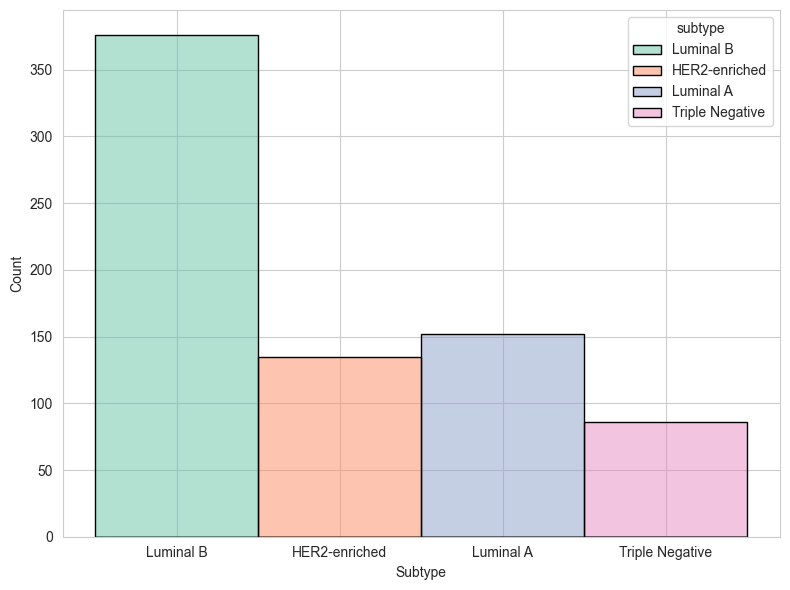
\includegraphics[width=\textwidth]{reports//assets/hist.png}
		\caption{Subtype distribution}
		\label{fig:subtype_hist}
	\end{subfigure}
	\begin{subfigure}[t]{0.49\textwidth}
		\centering
		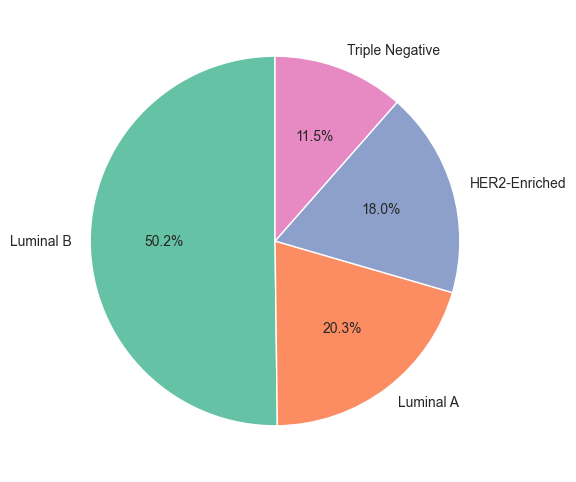
\includegraphics[width=\textwidth]{reports/assets/pie.png}
		\caption{Subtype distribution (pie chart)}
		\label{fig:subtype_pie}
	\end{subfigure}
	\caption[CMMD2 molecular subtypes distribution]{Subtype distribution of patients (CMMD2)}
	\label{fig:subtype_charts}
\end{figure}

\subsection{CMMD2 Limitations and Challenges}

Although CMMD2 is a valuable dataset for this study, it presents certain limitations that should be kept in mind:

\begin{enumerate}
    \item \textbf{Lack of region of interest (ROI) annotations}: The dataset does not provide annotated ROIs for tumor locations, which makes it challenging for machine learning models to focus on the relevant areas within the images.
    \item \textbf{Single image provider}: All mammograms were acquired using the same imaging device. As a result, models trained on this dataset may not generalize well to images obtained from different devices or providers.
    \item \textbf{High class imbalance}: As mentioned earlier, the dataset suffers from significant class imbalance. This can cause models to overfit to the dominant class, although it does reflect the real-world distribution of breast cancer molecular subtypes.
\end{enumerate}



\subsection{Examples of CMMD2 Images}

\begin{figure}[h!]
	\centering
	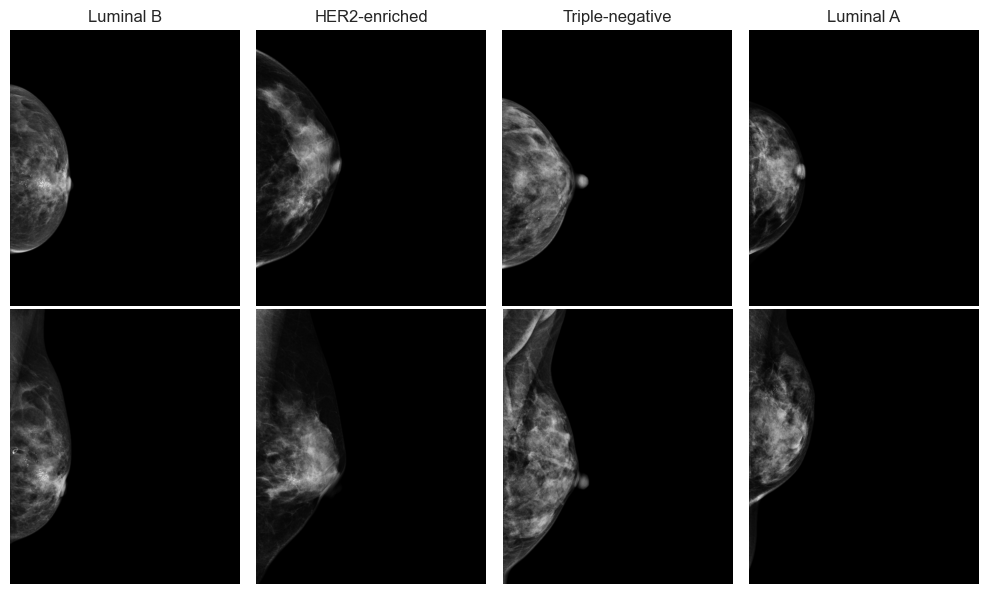
\includegraphics[width=1.0\linewidth]{reports//assets/images_examples.png}
	\caption[CMMD2 mammography images examples]{Example of mammography images of the CCMD2 dataset. Top row represent a CC view whereas bottom row illustrated a MLO view. Each column depicted one subtype of cancer.}
	\label{fig:cmmd-examples}
\end{figure}

\section{The TOMPEI-CMMD analysis}

The TOMPEI-CMMD is an enhanced analysis of the original CMMD dataset, developed by Kashiwada et al. (2025) \cite{kashiwada_tompei-cmmd_2025}. This enhancement was designed to provide comprehensive radiological insights and to enable a systematic re-evaluation of the existing mammographic images.

A board-certified radiologist with 20 years of experience in breast imaging assessed all images, documenting detailed radiological findings, including masses, calcifications, focal asymmetric densities, architectural distortions, and their anatomical locations. This new analysis also provides pixel-level segmentation masks for all identified findings in the MLO views, generated based on the radiologist’s expert assessment.

The TOMPEI-CMMD is valuable for this study because it also provides additional insights into the data in the CMMD2 subset, specifically regarding mammographies exclusions and laterality corrections guided by the expert radiologist. These enhancements further curate the CMMD2 dataset, improving its quality.

Table~\ref{tab:tompei_exclusions} summarizes the exclusion reasons identified during the TOMPEI-CMMD analysis, as well as the number of items affected in the CMMD2 subset.

\begin{table}[h!]
    \caption[TOMPEI-CMMD exclusion reasons]{Number of CMMD2 mammographies affected by each exclusion reason following the TOMPEI-CMMD analysis.}
    \centering
    \begin{tabular}{l p{6cm} c}
        \toprule
        \textbf{Exclusion reason} & \textbf{Description} & \textbf{Affected mammographies} \\
        \midrule
        CV Port & Presence of a central venous port visible in the mammography image. & 7 \\
        Lymphedema & Presence of lymphedema-related changes visible in the image. & 1 \\
        Neurofibromatosis & Presence of neurofibromatosis-related findings visible in the image. & 2 \\
        White objects & Presence of extraneous white objects or artifacts in the image. & 2 \\
        Invisible & Lesion not visible or undetectable in the mammography image. & 76 \\
        Benign & Lesion determined to be benign upon expert review. & 10 \\
        Normal & No abnormal findings detected in the image. & 724 \\
        \textbf{Total} &  & \textbf{824} \\
        \bottomrule
    \end{tabular}
    \label{tab:tompei_exclusions}
\end{table}

After applying all exclusions and performing 9 laterality corrections (where images were mislabeled), our final dataset is summarized in Table~\ref{tab:final_dataset_overview}.

\begin{table}[h!]
    \caption[Final Dataset Overview]{Final dataset overview after exclusions and corrections.}
    \centering
    \begin{tabular}{c c c}
    \toprule
    \textbf{Patients} & \textbf{Mammographies} & \textbf{Images} \\
    \midrule
    672 & 674 & 1348 \\
    \bottomrule
    \end{tabular}
    \label{tab:final_dataset_overview}
\end{table}

There are 672 unique patients in the final dataset. However, two patients were diagnosed with bilateral breast cancer\footnote{Cancer in both the left and right breasts.}, resulting in a total of 674 mammographies. As each mammography includes both CC and MLO views, the final dataset includes 1,348 images.


\section{Image Preprocessing}

To prepare the dataset for DL experiments, image preprocessing is essential. The original images are stored in DICOM (\texttt{.dcm}) format, and many include a substantial black background, which can negatively impact both computational efficiency and model performance if not addressed. The following preprocessing steps were applied, and the final result is illustrated in Figure~\ref{fig:preprocessing}:


\begin{enumerate}
    \item \textbf{Smart Cropping}: A heuristic algorithm \footnote{A practical, rule-based approach designed to quickly find a good solution to a problem when finding the optimal solution would be too complex or time-consuming.} was applied to automatically crop the majority of the black background from each image, retaining only the region containing breast tissue. This step maximizes the model's focus on relevant anatomical structures and reduces computational overhead.
    \item \textbf{Median Filtering}: A median filter was used to reduce noise while preserving edges and important details in the mammograms. This helps enhance image quality and supports more reliable feature extraction by DL models.
    \item \textbf{Image Conversion and Storage}: The preprocessed images were converted into a standard format (PNG) and stored in a more accessible directory. This step also facilitates efficient data loading and reproducibility in subsequent experiments.
\end{enumerate}


\begin{figure}[h!]
    \centering
    \begin{subfigure}[t]{0.35\textwidth}
        \centering
        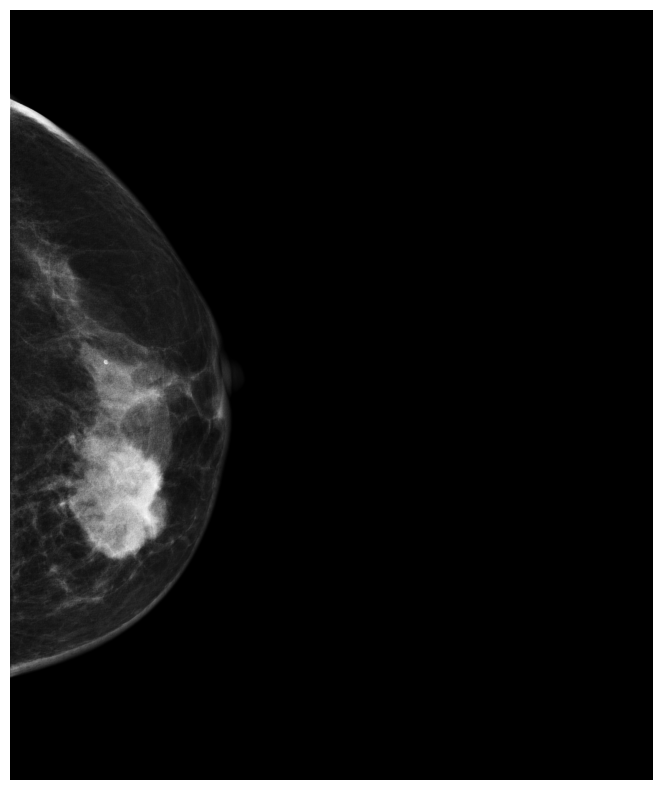
\includegraphics[width=\textwidth]{reports//assets/preprocess_a.png}
        \caption{}
        \label{fig:pre_original}
    \end{subfigure}
    \begin{subfigure}[t]{0.15\textwidth}
        \centering
        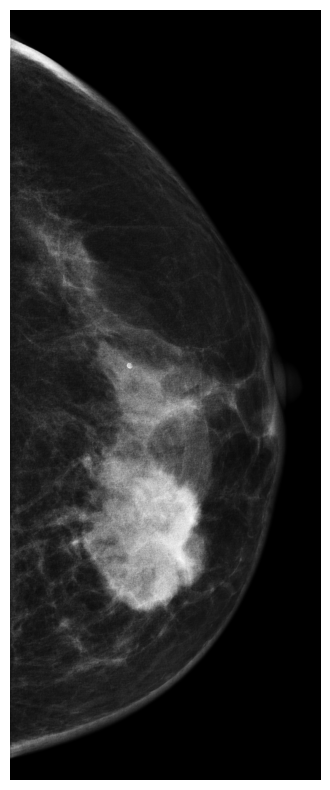
\includegraphics[width=\textwidth]{reports//assets/preprocess_b.png}
        \caption{}
        \label{fig:pre_cropped}
    \end{subfigure}
    \begin{subfigure}[t]{0.15\textwidth}
        \centering
        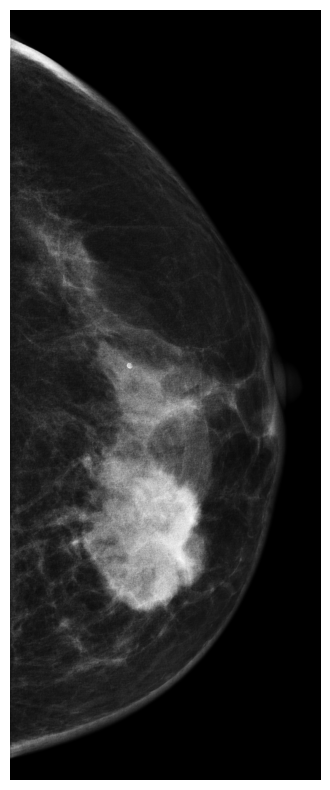
\includegraphics[width=\textwidth]{reports//assets/preprocess_c.png}
        \caption{}
        \label{fig:pre_mean}
    \end{subfigure}
   \caption[Preprocessing pipeline result]{Illustration of the preprocessing pipeline result: (a) original image, (b) image after cropping, and (c) image after median filter application.}
    \label{fig:preprocessing}
\end{figure}

After applying this preprocessing pipeline, the resulting folder directory is as follows. Each image is stored within a folder labeled with the corresponding patient identification:

\vspace{0.5cm}
\dirtree{%
.1 data/.
.2 preprocessed.
.3 D2-0001.
.4 CC-L.png.
.4 MLO-L.png.
.3 D2-0002.
.3 ....
}

In addition to these preprocessing steps, a histogram standardization\footnote{Histogram standardization is a technique used to adjust the intensity values of an image so that its histogram has a specified mean and variance, usually mean 0 and variance 1. This helps to make images from different sources more comparable and consistent for further analysis.} technique is also applied. However, this is performed during the data splitting phase to avoid data leakage \footnote{When information that would not be available at prediction time is unintentionally used during model training. This leads to overly optimistic performance during evaluation but poor results in real-world use, because the model has learned patterns it should not have access to}. Details regarding this procedure will be discussed in the following section.


\section{Data splitting and stratification}

Once images are preprocessed, the next step is to create training and testing splits of the data. In DL, it is standard practice to divide the dataset into separate subsets to accurately assess model performance and prevent overfitting, ensuring that the model generalizes well to unseen data \cite{noauthor_data_nodate}. In particular, three key points must be addressed:

\begin{itemize}
\item Ensure reproducibility of experiments.
\item Keep the same data distribution across splits (stratification) to ensure balanced representation of classes.
\item Avoid data leakage by ensuring that no information from the test set is used during training.
\end{itemize}

\subsection{Repeated holdout strategy}

To best assess the model's performance, the repeated holdout strategy was used. Also known as Monte Carlo Cross-Validation, this approach consists of randomly splitting the dataset into training and testing sets multiple times, resulting in different train-test splits for each iteration. The model is trained and evaluated on each split, and the results are averaged to provide a more robust estimate of performance \cite{marzbanAllModelsAre2020}.

In this study, \textbf{three different train-test splits consisting of 80\% training and 20\% test data were used}. Each split was generated with a different fixed random seed (0, 21, and 42) to ensure reproducibility of the data splitting process. For clarity, each split is named according to its corresponding seed (e.g., Split 0).

\subsection{Data distribution}

To ensure consistent data distribution across the different train-test splits, stratification was performed based on the molecular subtype annotations. This guaranteed that each train and test split maintained a similar proportion of each molecular subtype, thereby reducing the risk of biased performance estimates due to class imbalance. The resulting data distributions for the three train-test splits are shown in Figure~\ref{fig:pie_dist} and Figure~\ref{fig:pie_hist}, along with additional insights regarding image overlap.

\subsection{Avoiding Data Leakage}

To avoid data leakage, the splits were performed at the patient level. This means that patient identification was used to ensure that all samples from a given patient were assigned exclusively to either the training or test set, preventing any overlap between the two. This consideration was included in the training, where employing a Stratified Grouped K-Fold ensured no patient data leaked between folds.

\subsection{Histogram Standardization} 

Histogram standardization is an important preprocessing step that equalizes image intensities to reduce variability, even within datasets acquired from a single device such as CMMD2. This technique has been shown to improve domain generalization and model performance \cite{garruchoDomainGeneralizationDeep2022}. In this study, histogram standardization was applied after data splitting, following the repeated holdout strategy. For each train-test split, intensity landmarks were learned from the training set and then applied to standardize both the training and test images. An example of the effect of this technique on image appearance and intensity distribution is shown in Figure~\ref{fig:standardized_examples}.


\begin{figure}[h!]
    \centering
    \begin{subfigure}[t]{1.0\textwidth}
        \centering
        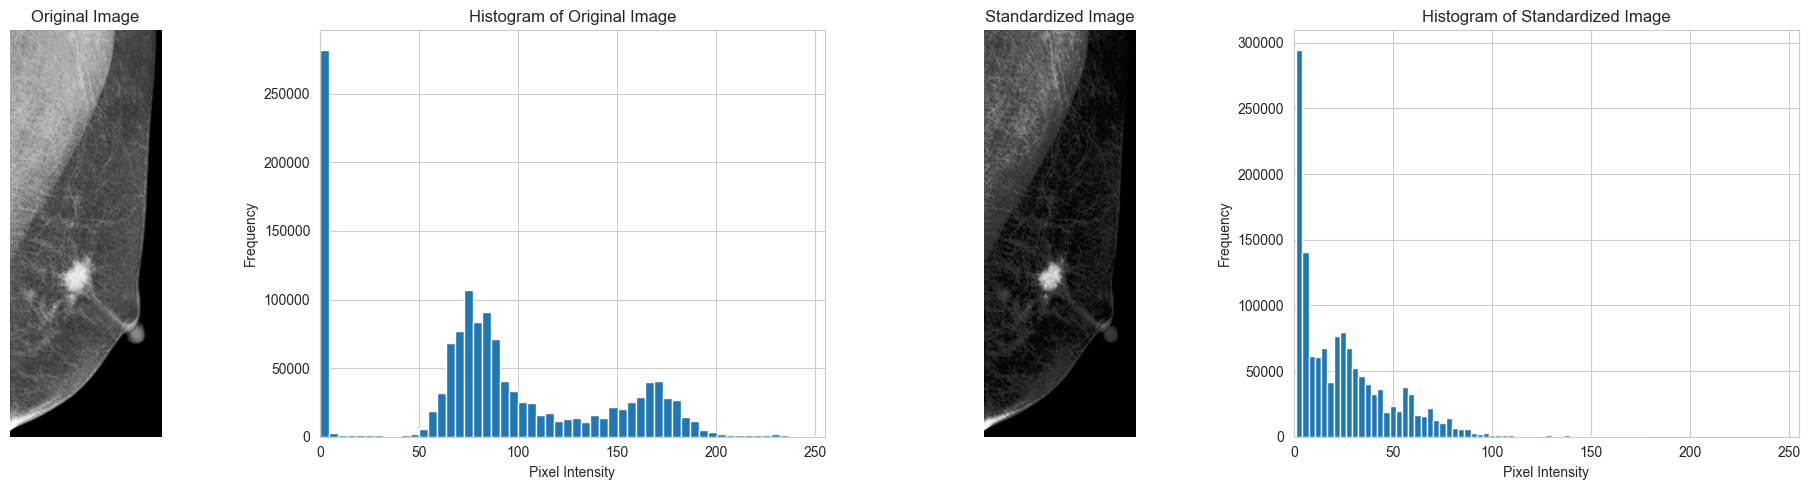
\includegraphics[width=\textwidth]{reports//assets/standarized1.png}
        \label{fig:standarized_1}
    \end{subfigure}
    \begin{subfigure}[t]{1.0\textwidth}
        \centering
        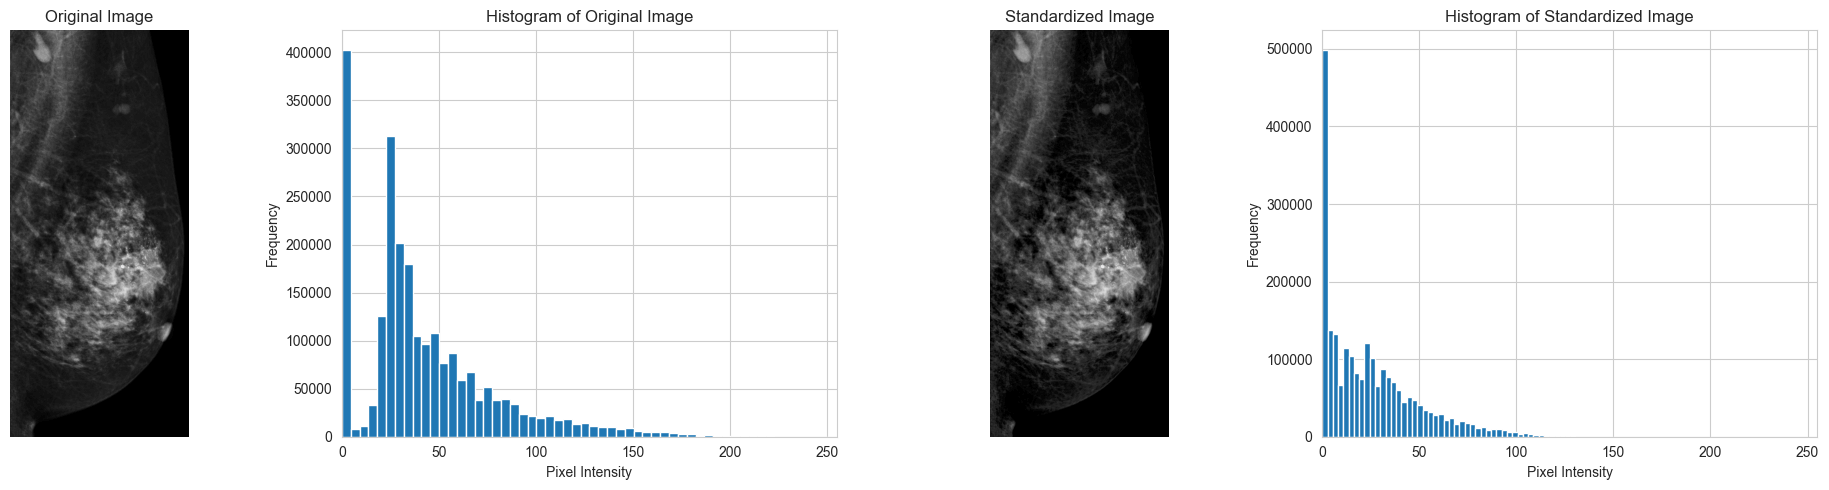
\includegraphics[width=\textwidth]{reports//assets/standarized2.png}
        \label{fig:standardized_2}
    \end{subfigure}
    \caption[Histogram standardization result]{Example of an image before and after applying histogram standardization. The histograms demonstrate how intensity distributions become more similar after standardization.}
    \label{fig:standardized_examples}
\end{figure}

\subsection{Final splits overview}

Following preprocessing, data splitting, and histogram standardization, the images were systematically organized by seed, split, and subtype to enable efficient data loading during training. The final image format chosen was \texttt{.npy}\footnote{NumPy binary format}, due to its capability for efficient storage, rapid loading of large arrays, and preservation of exact intensity values, including standardized histogram ranges, without any loss or alteration. The directory structure of the splits is presented as follows:

\vspace{0.5cm}
\dirtree{%
.1 splits/.
.2 SEED0.
.3 train.
.4 her2-enriched.
.5 D2-0001-CC-R.npy.
.4 luminal-a.
.4 luminal-b.
.4 triple-negative.
.3 test.
.2 SEED21.
.2 SEED42.
}

\section{Evaluation Metrics}

Selecting appropriate evaluation metrics is essential for accurately assessing model performance, especially in multiclass classification tasks like distinguishing breast cancer molecular subtypes. To ensure consistency with recent studies, such as those by Mota et al.\ \cite{mota_breast_2024} and Rabah et al.\ \cite{ben_rabah_multimodal_2025}, this work reports metrics including AUC, Precision, Recall, and F1-Score, with an emphasis on macro-averaged values. Macro-averaging treats each class equally by averaging metrics calculated independently for each class, which is particularly important given the high class imbalance in the dataset. 

Additionally, Cohen’s Kappa coefficient is included to measure agreement between predicted and true labels, accounting for chance. To further address class imbalance, Balanced Accuracy is reported instead of standard accuracy. For metrics visualization, the ROC AUC curve was used to compare the overall results of this metric and a confusion matrix \cite{noauthor_que_nodate} to evaluate predictions.

Table \ref{tab:metrics_overview} summarizes the evaluation metrics used in this study:

\begin{table}[h!]
\centering
\caption[Metrics Overview]{Overview of evaluation metrics used in this work. All metrics except AUC and Cohen's Kappa are reported as macro-averaged values.}
\begin{tabularx}{\textwidth}{l X X}
\toprule
\textbf{Metric} & \textbf{Formula} & \textbf{Description} \\
\midrule
    Balanced Accuracy &
    $\frac{1}{N}\sum_{i=1}^N \frac{TP_i}{TP_i + FN_i}$ &
    Average recall across all classes; robust to class imbalance.  \\
    Macro Precision &
    $\frac{1}{N}\sum_{i=1}^N \frac{TP_i}{TP_i + FP_i}$ &
    Average of per-class precision; treats all classes equally.  \\
    Macro Recall (Sensitivity) &
    $\frac{1}{N}\sum_{i=1}^N \frac{TP_i}{TP_i + FN_i}$ &
    Average of per-class recall; treats all classes equally.  \\
    Macro F1-Score &
    $\frac{1}{N}\sum_{i=1}^N 2 \cdot \frac{\text{Precision}_i \cdot \text{Recall}_i}{\text{Precision}_i + \text{Recall}_i}$ &
    Average of per-class F1-scores; balances precision and recall.  \\
    Cohen's Kappa &
    $\frac{p_o - p_e}{1 - p_e}$ &
    Measures agreement between predictions and true labels, adjusted for chance.  \\
    Macro AUC (ROC) &
    --- &
    Average area under the ROC curve for each class; measures the ability to distinguish between classes.  \\
\bottomrule
\end{tabularx}
\label{tab:metrics_overview}
\end{table}

\section{Model Architectures and Pipeline}

\subsection{Models Backbones Selection}

For this study, the model architectures (backbones) were selected using the \textit{timm} library \cite{TimmPyTorchImage2025}, which provides a wide range of state-of-the-art pretrained models for image classification.

\begin{itemize}
    \item \textbf{ResNet-101}: timm/resnet101
    \item \textbf{ViT}: timm/vit\_base\_patch16\_384
    \item \textbf{MaxVit}: timm/maxvit\_small\_tf\_384
    \item \textbf{Swin}: timm/swin\_base\_patch4\_window12\_384
\end{itemize}


\subsection{Models input format}

Defining the input shape is essential when working with pretrained models, as they are typically trained on benchmark datasets with fixed input sizes such as 224×224, 384×384 or 512×512. To ensure a fair comparison across all four architectures, we standardized the input size to 384×384×3 (RGB). This decision is supported by empirical evidence showing that transformer-based models achieve optimal performance at higher resolutions, while CNNs like ResNet101 are flexible and also benefit from larger images.

Since the dataset does not provide region of interest (ROI) annotations, as said earlier, we apply a transformation pipeline that first resizes each image so that its smallest dimension matches 384 pixels, preserving the original aspect ratio, and then applies a center crop to obtain a 384×384 patch. This straightforward approach is effective in practice and is illustrated in Figure~\ref{fig:384_patches}.

\begin{figure}[h!]
    \centering
    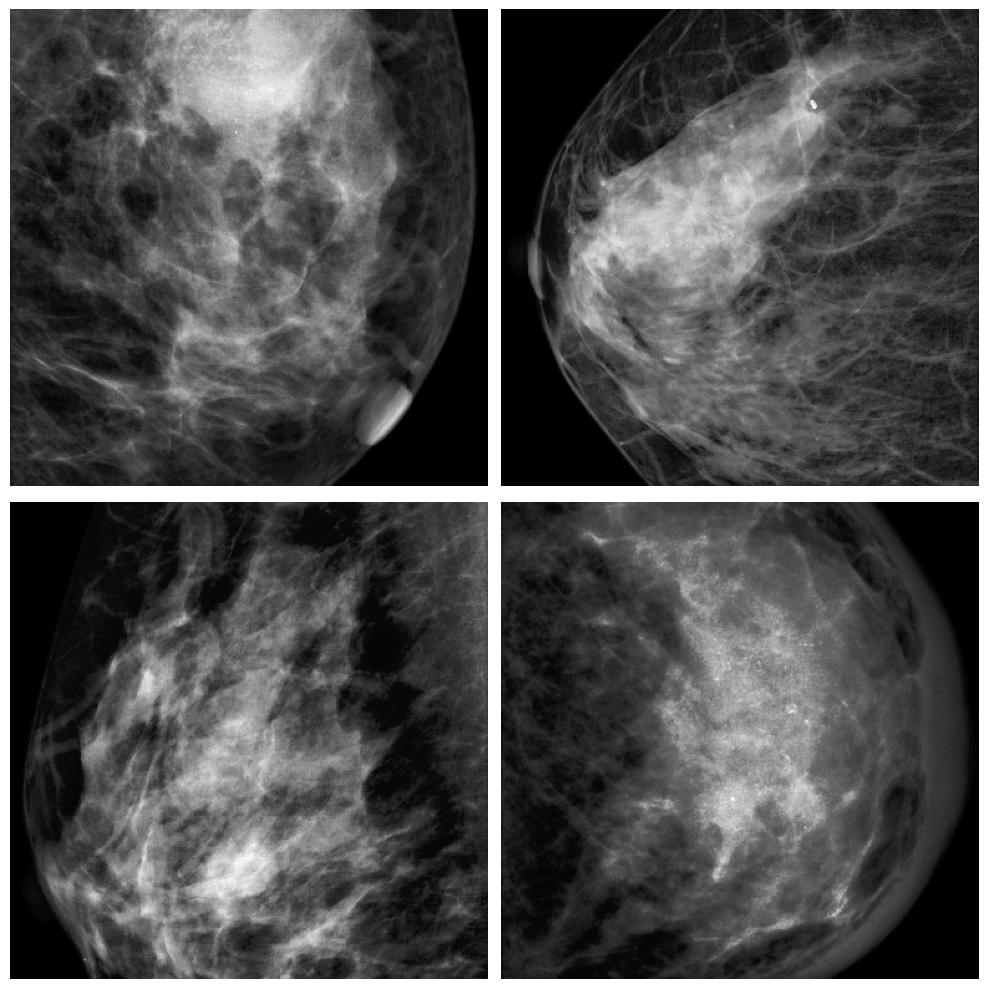
\includegraphics[width=0.3\linewidth]{reports//assets/384patchs.png}
    \caption[Input 384×384 patches]{Examples of centered 384×384 patches extracted from the original images, which are then converted to tensors for model input.}
    \label{fig:384_patches}
\end{figure}

\subsection{Model Output Format}

After processing an input image, each model produces a one-dimensional tensor containing the predicted probabilities for each of the four molecular subtypes. This means that for every image, the model assigns a likelihood to each subtype, reflecting its confidence in the classification. These probabilities are calculated using a softmax activation function in the final layer, ensuring that all values sum to one and can be interpreted as true probabilities. The subtype with the highest probability is then selected as the model’s final prediction for that case.

By adopting this standardized output format across all models, we make it easy to compare their predictions directly and to apply consistent evaluation metrics. This approach not only streamlines the analysis but also ensures that differences in performance can be attributed to the models themselves, rather than to variations in output processing. Figure~\ref{fig:flowchart} provides a high-level overview of the inference process, from image input to final subtype prediction.

\begin{figure}[h!]
    \centering
    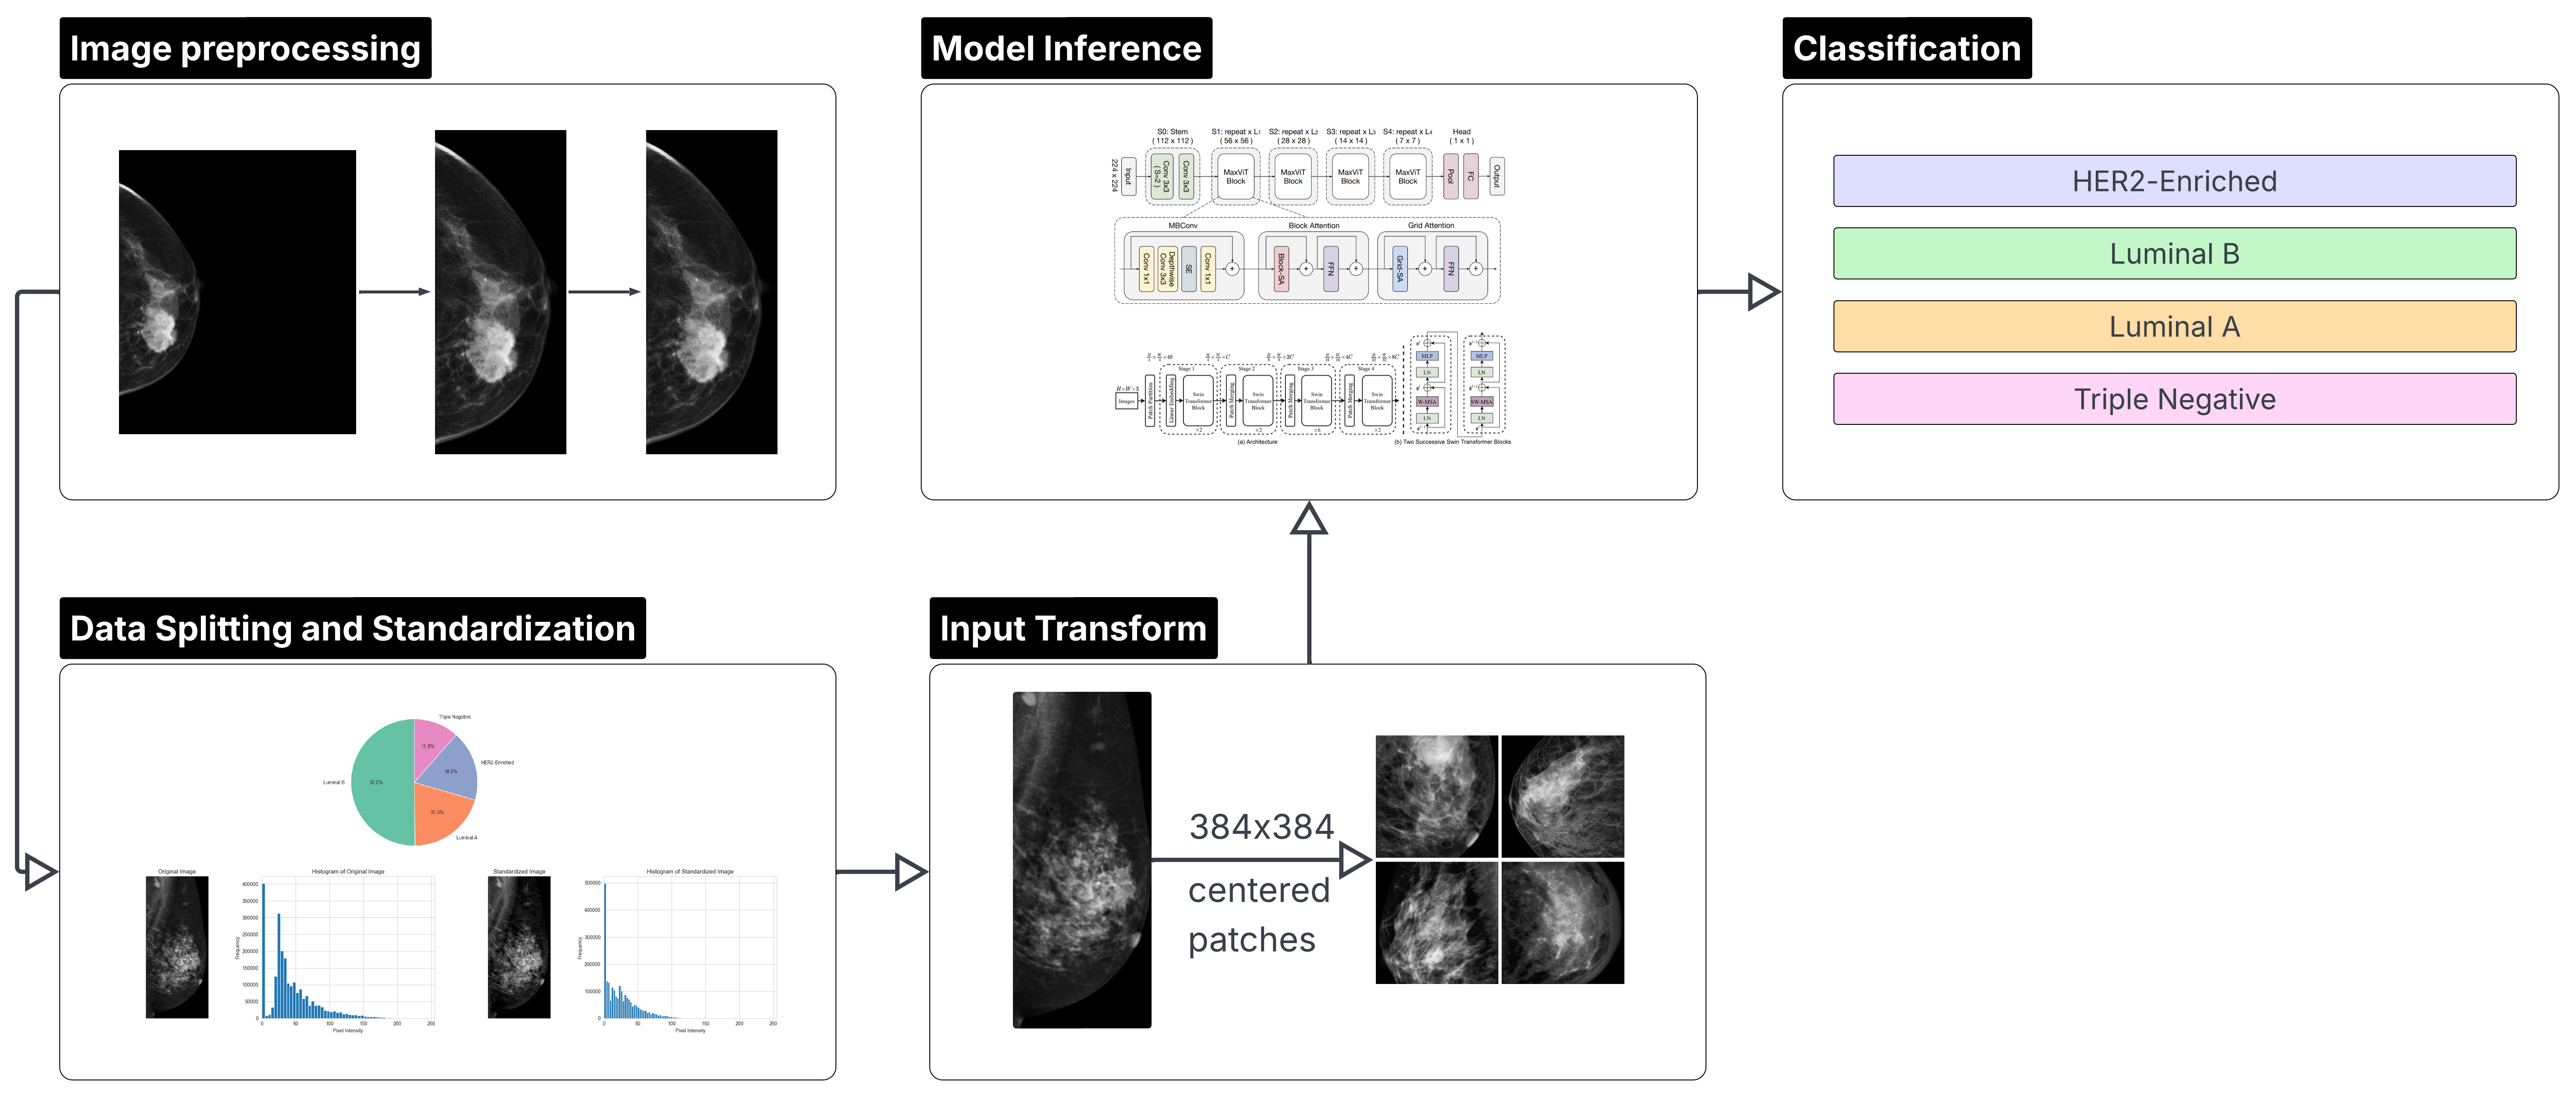
\includegraphics[width=0.9\linewidth]{reports//assets/Flowchart.png}
    \caption[Workflow pipeline]{Overview of the workflow pipeline for model inference after training and evaluation.}
    \label{fig:flowchart}
\end{figure}

\section{Experiments}

This section presents the experimental design employed to compare the performance of the four models (ResNet-101, ViT, Swin, and MaxViT). Common guidelines and configurations applied across all experiments are detailed, along with the different modalities evaluated using three distinct train-test splits.

\subsection{Evaluation Pipeline}

To systematically evaluate model performance in classifying breast cancer molecular subtypes, four training modalities were proposed. Each modality is designed to address and mitigate class imbalance within the dataset as effectively as possible:

\begin{itemize}
    \item Weighted loss without image augmentation
    \item Weighted loss with image augmentation
    \item Oversampling without image augmentation
    \item Oversampling with image augmentation
\end{itemize}

Each modality is applied to all four models using a 3-fold cross-validation strategy on the training set, and this process is repeated for each of the three different train-test splits.Validation metrics from the cross-validation are collected and summarized for each train-test split, providing the basis for subsequent statistical analysis.Based on the results of this analysis, the best-performing training modalities are selected for fine-tuning on the entire training set, followed by evaluation on the corresponding test holdout set for each split. In total, the evaluation required \textbf{144 experiments}, calculated as 4 models × 3 folds × 4 modalities × 3 train-test splits. The overall pipeline can be summarized as follows:

\begin{enumerate}[label=\textbf{Step \arabic*}:]
    \item Select a train-test split (e.g., SPLIT0).
    \item Select a model backbone (ResNet-101, ViT, Swin, or MaxViT).
    \item Evaluate the model using each of the four training modalities with 3-fold cross-validation.
    \item Collect validation metrics for each modality, seed, model, and fold.
    \item Repeat the process for all train-test splits and models.
\end{enumerate}

\subsection{Common Hyperparameters}

A set of common training hyperparameters was selected to ensure they were suitable for all model types evaluated in this study. Table~\ref{tab:hyperparams} summarizes the hyperparameters used.


\begin{table}[h!]
    \caption[Common training hyperparameters]{Common training hyperparameters.}
    \centering
    \begin{tabular}{l l}
        \toprule
        \textbf{Hyperparameter} & \textbf{Value} \\
        \midrule
        Optimizer  & AdamW \\

        Learning Rate  & 1e-4 (1e-5 for fine-tuning) \\
 
        Weight Decay (L2-Regularization) & 1e-2 \\

        LR Scheduler & OneCycleLR \\
   
        Batch Size & 32 \\

        Epochs & 100 (max) \\
        \bottomrule
    \end{tabular}
    \label{tab:hyperparams}
\end{table}

\subsection{Experiment modalities}

\subsubsection{Using image augmentation}

Image augmentation is a technique used to increase the diversity and size of a dataset by generating modified versions of existing images in memory through various transformations or contrast adjustments~\cite{noauthor_complete_nodate}. For model training, only slight transformations were applied, including horizontal flipping (50\%), rotations between $-10^\circ$ and $10^\circ$ (30\%), and CLAHE (10\%)\footnote{Contrast Limited Adaptive Histogram Equalization, an advanced image processing technique used to enhance local image contrast.}. These augmentations are medically safe and help the models generalize better and mitigate class imbalance. Figure \ref{fig:augmentations} illustrates these augmentations.

\begin{figure}[h!]
    \centering
    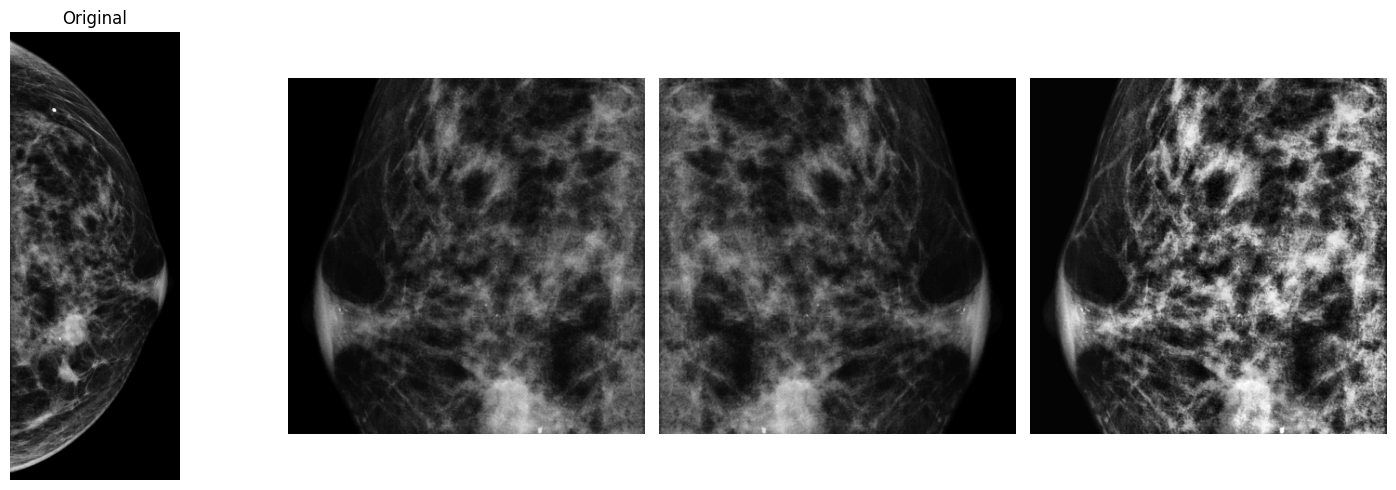
\includegraphics[width=0.8\linewidth]{reports//assets/augmentations.png}
    \caption[Image augmentations]{Image augmentations example.}
    \label{fig:augmentations}
\end{figure}


\textbf{Using Weighted Cross-entropy Loss}

The Cross-Entropy loss is a function to measure the difference between predicted and actual class distributions. The weighted version applies  a scaling factor (typically the inverse  of class frequencies) to address class imbalance effectively or emphasize certain classes during model training. Mathematically can be expressed as:

\begin{equation}
J_{\text{WCE}} = -\frac{1}{M} \sum_{m=1}^{M} \sum_{k=1}^{K} w_k \; y_{m,k} \; \log\left( h_\theta(x_m, k) \right)
\end{equation}

Where: $J_{\text{WCE}}$~: weighted cross-entropy loss, $M$~: number of samples in the batch, $K$~: number of classes, $w_k$~: weight for class~$k$, $y_{m,k}$~: indicator (1 if sample~$m$ belongs to class~$k$, else~0), and $h_\theta(x_m, k)$~: predicted probability for class~$k$ (softmax output).

This loss function can help significantly improve model performance in imbalanced datasets.

\textbf{Using Weighted Random Sampler}

Weighted random sampling is another technique to mitigate class imbalance. In this approach, sampling probabilities are assigned based on the inverse frequency of each class, giving samples from minority classes a higher probability of selection during batch training compared to samples from majority classes. This is especially useful in datasets like CMMD2, where one class, such as Luminal B, dominates and has significantly more samples than the others.

However, a key limitation is that weighted random sampling should not be combined with weighted cross-entropy loss, as both techniques address class imbalance and using them together can lead to overcompensation, potentially introducing bias during training. For this reason, weighted random sampling is implemented as a separate experimental modality. Figure~\ref{fig:batch_sampling} shows the typical class distribution within a batch (batch size 32), while Figure~\ref{fig:batch_sampling_weighted} illustrates the batch distribution after applying the Weighted Random Sampler.

\begin{figure}[h!]
    \centering
    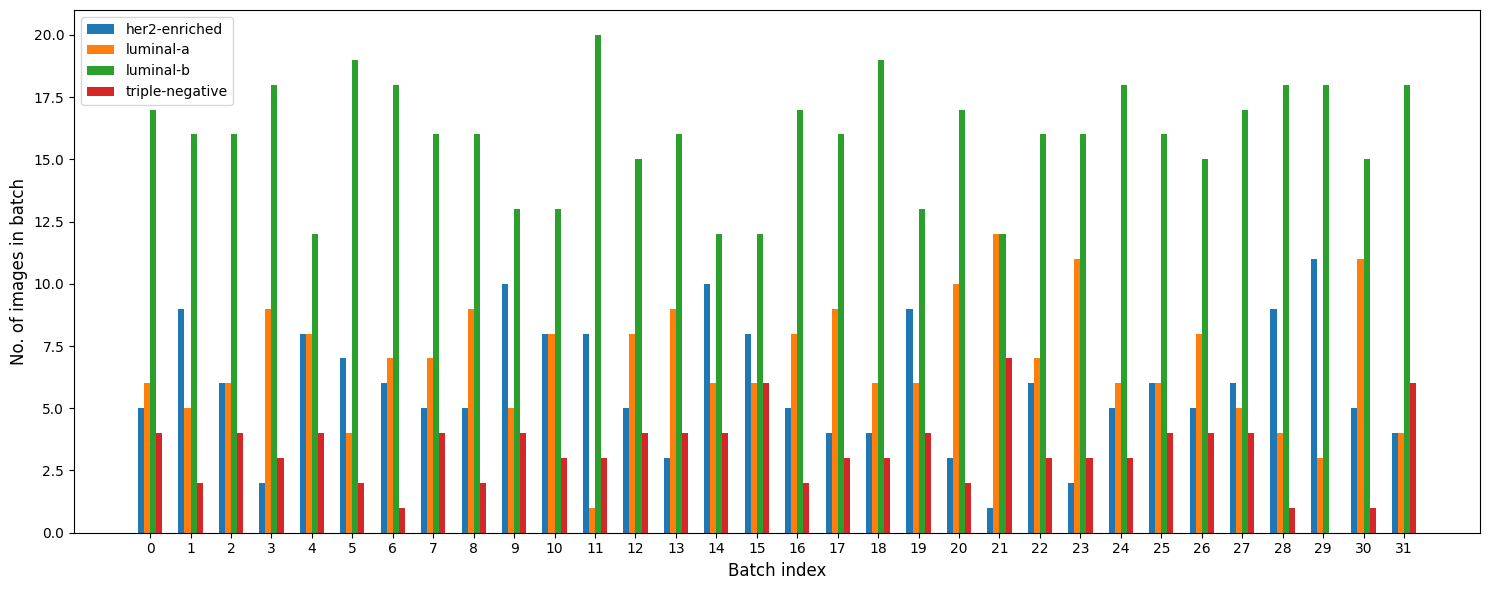
\includegraphics[width=.8\linewidth]{reports//assets/sampler.png}
    \caption[Batch Sampling (Default)]{Class distribution within a typical batch (batch size = 32) during a training epoch using default sampling. The average number of images per batch for each class is: HER2: 6.03, LumA: 6.72, LumB: 15.75, and TN: 3.50.}
    \label{fig:batch_sampling}
\end{figure}

\begin{figure}[ht!]
    \centering
    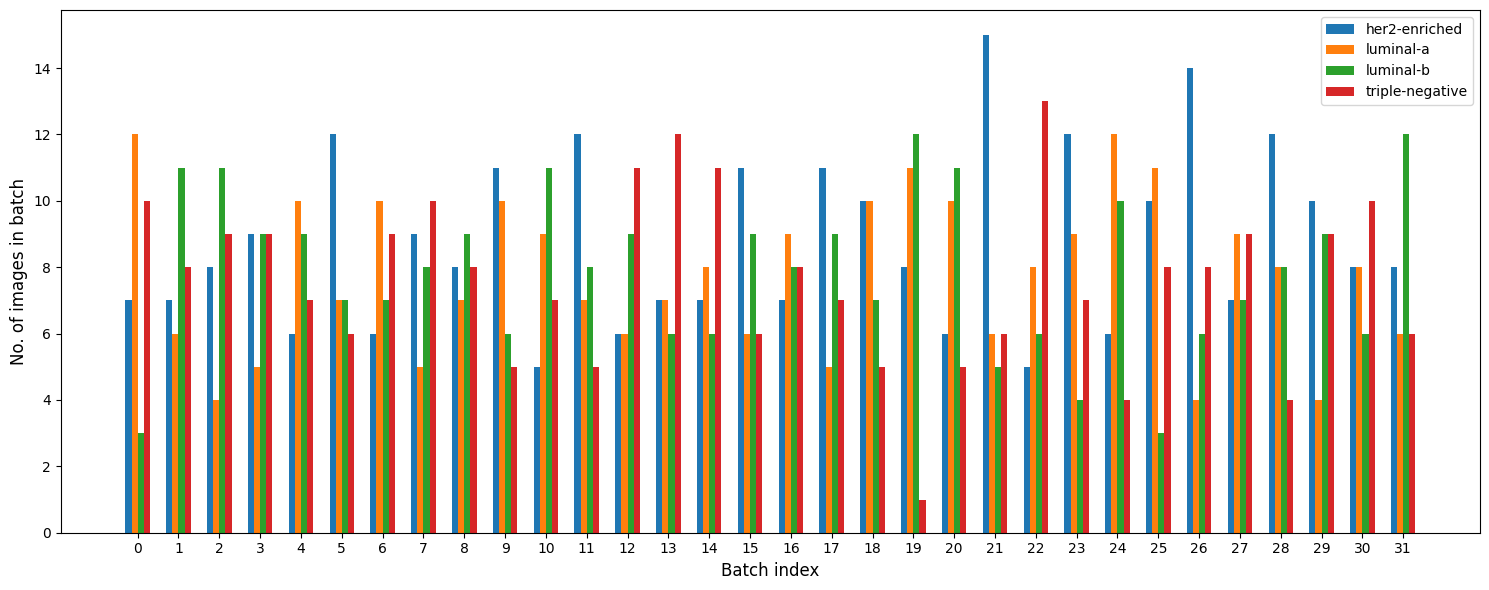
\includegraphics[width=0.8\linewidth]{reports//assets/sampler2.png}
    \caption[Batch Sampling (Weighted)]{Class distribution within a batch (batch size = 32) after applying weighted random sampling. The average number of images per batch for each class is: HER2: 8.25, LumA: 7.88, LumB: 7.28, and TN: 8.59.}
    \label{fig:batch_sampling_weighted}
\end{figure}


\subsection{Statistical Test}

After completing the experiments, this should be evaluated statistically. In studies of this nature, it is common practice to apply statistical methods to determine whether observed differences in model performance are significant or could have occurred by chance. The common methodology involves a two-step statistical analysis. For this study, a Friedman test was performed first to assess overall differences among models, followed by Wilcoxon signed-rank tests for pairwise comparisons between models \cite{demsar_statistical_2006}.

\subsubsection{Friedman Test}

The Friedman test is a simple, non-parametric statistical\footnote{Non-parametric methods are statistical techniques that do not assume a specific distribution for the data, making them suitable for non-normal or ordinal data.} test used to compare three or more related groups. The null hypothesis is that all models perform equally, meaning there are no significant differences in their median performance across repeated measurements \cite{demsar_statistical_2006}. To perform the test, each model’s performance (e.g., AUC) is ranked within each experimental unit (such as each combination of fold, seed, and modality). Then, the test statistic is calculated as:

\begin{equation}
\chi^2_F = \frac{12}{nk(k+1)} \sum_{j=1}^{k} R_j^2 - 3n(k+1)
\end{equation}

\noindent
Where $n$ is the number of experimental units, $k$ is the number of models being compared, and $R_j$ is the sum of ranks for model $j$. This statistic follows a chi-square distribution with $k-1$ degrees of freedom. If the resulting p-value\footnote{A measure of how likely your observed results are if there were no real difference or effect.} is less than 0.05, the null hypothesis can be rejected.

\subsubsection{Wilcoxon Signed-Rank Test}

The Wilcoxon signed-rank test is a non-parametric test used to determine if there is a statistically significant difference between two sets of paired or related values by ranking the absolute differences between each pair, then comparing the sums of the positive and negative ranks to assess whether the observed differences are likely due to chance or reflect a true effect \cite{demsar_statistical_2006}. The test statistic is defined as:

\begin{equation}
W = \min \left( W^+,\, W^- \right)
\end{equation}


Where $W^+$ is the sum of the ranks for the positive differences, and $W^-$ is the sum of the ranks for the negative differences.


\chapter{Results and Discussion}

This chapter presents the main findings of the study, including the performance evaluation of the proposed models and training modalities for breast cancer molecular subtyping using mammographic images. The results are analyzed using the evaluation metrics and statistical methods described in previous chapters. Comparative analyses highlight the strengths and limitations of each approach, and the implications of these findings are discussed in the context of current research.

\section{Experiments Results}

A total of 144 experiments were conducted to collect cross-validation metrics. As defined earlier, each model was trained using 3-fold cross-validation, recording validation metrics for each fold across 3 distinct train-test splits (seeds 0, 21, and 42) and 4 different modalities. To ensure the reliability of the results, each experiment used the same seed for the K-Fold partitioning, guaranteeing consistent data splits across all runs. The complete set of results is presented in Table~\ref{tab:complete_metrics}, while the results averaged by seed are shown in Tables~\ref{tab:avg_metrics_seed_0}, \ref{tab:avg_metrics_seed_21}, and \ref{tab:avg_metrics_seed_42}. To provide an overview of the validation metrics obtained from K-Fold cross-validation for each seed, Table~\ref{tab:per_seed_metrics_avg} presents the averaged values.


\begin{scriptsize}
\begin{longtable}{@{}l l p{0.6cm} p{1.5cm} p{1.5cm} p{1.5cm} p{1.5cm} p{1.5cm}@{}}
\caption[Average validation metrics per seed]{Average per seed validation metrics obtained after 3 Folds cross validation in 3 different train-test splits.}
\label{tab:per_seed_metrics_avg}\\
\toprule
\textbf{Model} & \textbf{Sampling} & \textbf{Aug.} &
\textbf{B.\ Acc.} & \textbf{AUC} & \textbf{F1} &
\textbf{Prec.} & \textbf{C.\ Kappa} \\
\midrule
\endfirsthead

\toprule
\textbf{Model} & \textbf{Sampling} & \textbf{Aug.} &
\textbf{B.\ Acc.} & \textbf{AUC} & \textbf{F1} &
\textbf{Prec.} & \textbf{C.\ Kappa} \\
\midrule
\endhead

\midrule
\multicolumn{8}{r}{\textit{Continued on next page}}\\
\midrule
\endfoot

\bottomrule
\endlastfoot
ResNet101 & Weighted    & No  & 0.2977 $\pm$ 0.032  & 0.5649 $\pm$ 0.0307 & 0.2788 $\pm$ 0.0345 & 0.2842 $\pm$ 0.0356 & 0.0734 $\pm$ 0.0409 \\
ResNet101 & Weighted    & Yes & 0.3133 $\pm$ 0.0158 & 0.5692 $\pm$ 0.0215 & 0.2941 $\pm$ 0.0213 & 0.3037 $\pm$ 0.0218 & 0.0931 $\pm$ 0.0250 \\
ResNet101 & Oversampled & No  & 0.2971 $\pm$ 0.0259 & 0.5619 $\pm$ 0.0294 & 0.2699 $\pm$ 0.0333 & 0.3049 $\pm$ 0.0295 & 0.0677 $\pm$ 0.0384 \\
ResNet101 & Oversampled & Yes & 0.3002 $\pm$ 0.0298 & 0.5681 $\pm$ 0.0241 & 0.2530 $\pm$ 0.0489 & 0.3229 $\pm$ 0.0777 & 0.0647 $\pm$ 0.0421 \\
ViT       & Weighted    & No  & 0.3319 $\pm$ 0.0439 & 0.5852 $\pm$ 0.0202 & 0.3002 $\pm$ 0.0450 & 0.3158 $\pm$ 0.0457 & 0.0888 $\pm$ 0.0466 \\
\textbf{ViT} & \textbf{Weighted} & \textbf{Yes} &
\textbf{0.3397 $\pm$ 0.0255} & \textbf{0.5864 $\pm$ 0.0202} &
\textbf{0.3062 $\pm$ 0.0467} & \textbf{0.3313 $\pm$ 0.0338} &
\textbf{0.1066 $\pm$ 0.0436} \\
ViT       & Oversampled & No  & 0.3134 $\pm$ 0.0378 & 0.5821 $\pm$ 0.0235 & 0.2816 $\pm$ 0.0273 & 0.3178 $\pm$ 0.0304 & 0.0719 $\pm$ 0.0367 \\
ViT       & Oversampled & Yes & 0.3214 $\pm$ 0.0293 & 0.5820 $\pm$ 0.0172 & 0.2923 $\pm$ 0.0406 & 0.3082 $\pm$ 0.0347 & 0.0867 $\pm$ 0.0362 \\
Swin      & Weighted    & No  & 0.3212 $\pm$ 0.0292 & 0.5819 $\pm$ 0.0193 & 0.2836 $\pm$ 0.0355 & 0.3083 $\pm$ 0.0207 & 0.0814 $\pm$ 0.0334 \\
Swin      & Weighted    & Yes & 0.3170 $\pm$ 0.0232 & 0.5825 $\pm$ 0.0169 & 0.2811 $\pm$ 0.0327 & 0.3051 $\pm$ 0.0254 & 0.0812 $\pm$ 0.0288 \\
Swin      & Oversampled & No  & 0.3152 $\pm$ 0.0183 & 0.5775 $\pm$ 0.0161 & 0.2838 $\pm$ 0.0325 & 0.3132 $\pm$ 0.0157 & 0.0790 $\pm$ 0.0180 \\
Swin      & Oversampled & Yes & 0.3143 $\pm$ 0.0211 & 0.5820 $\pm$ 0.0208 & 0.2806 $\pm$ 0.0391 & 0.3147 $\pm$ 0.0272 & 0.0812 $\pm$ 0.0317 \\
MaxVit    & Weighted    & No  & 0.3155 $\pm$ 0.0086 & 0.5776 $\pm$ 0.0171 & 0.3010 $\pm$ 0.0103 & 0.3098 $\pm$ 0.0116 & 0.0618 $\pm$ 0.0210 \\
MaxVit    & Weighted    & Yes & 0.3140 $\pm$ 0.0261 & 0.5836 $\pm$ 0.0255 & 0.2875 $\pm$ 0.0343 & 0.3119 $\pm$ 0.0332 & 0.0686 $\pm$ 0.0371 \\
MaxVit    & Oversampled & No  & 0.3157 $\pm$ 0.0270 & 0.5799 $\pm$ 0.0202 & 0.2886 $\pm$ 0.0240 & 0.2969 $\pm$ 0.0212 & 0.0649 $\pm$ 0.0322 \\
MaxVit    & Oversampled & Yes & 0.3107 $\pm$ 0.0355 & 0.5805 $\pm$ 0.0248 & 0.2896 $\pm$ 0.0297 & 0.3096 $\pm$ 0.0283 & 0.0637 $\pm$ 0.0438 \\
\end{longtable}
\end{scriptsize}


From these averaged results, it is notable that the best-performing model is ViT, which achieves the highest validation metrics, particularly in the modality using Weighted Cross-Entropy Loss and Data Augmentation. Although the results are modest and both training and validation were performed using only the classifier head, this provides an initial indication of the model's general performance. Focusing solely on the AUC score, the best-performing models and modalities are presented in Table \ref{tab:best_auc_modalities_validation}.

\begin{table}[h!]
  \centering
\caption[Best validation AUC scores by model and modality.]{Best validation AUC scores by model and modality.}
  \label{tab:best_auc_modalities_validation}
  \begin{tabular}{l l c c}
    \toprule
    \textbf{Model} & \textbf{Sampling} & \textbf{Augmentation} & \textbf{AUC} \\ 
    \midrule
    ViT & Weighted & Yes & 0.5864  $\pm$ 0.0202   \\
    MaxVit  & Weighted & Yes  & 0.5836 $\pm$  0.0255 \\
    Swin    & Weighted & Yes  & 0.5825 $\pm$  0.0169 \\
    ResNet-101    & Oversample & No & 0.5681 $\pm$  0.0241 \\
    \bottomrule
  \end{tabular}
\end{table}


Although these scores are quite low, this is understandable given the inherent difficulty of multiclass classification and the high heterogeneity of molecular subtypes. Nevertheless, based on these insights alone, we can suspect that our study hypothesis (that transformer-based models generalize somewhat better than our CNN baseline) is supported. The differences in performance across the three folds, particularly in metrics such as AUC and F1-score, suggest that transformer-based models may be capturing more complex patterns when classifying molecular subtypes compared to the ResNet-101 architecture.

To ensure these findings are not due to random chance or experimental variability, a statistical significance test was performed. Specifically, a Friedman test was applied to all collected validation metrics (Table \ref{tab:complete_metrics}). This test determines whether there are statistically significant differences among the experiments for each metric, with significance indicated by a p-value less than 0.05. Table \ref{tab:friedman_test_results} summarizes these results.

\begin{table}[h!]
  \centering
\caption[Summary of Friedman test statistics and p-values for all evaluation metrics.]{Friedman test statistics and corresponding p-values for different evaluation metrics comparing model and modality performance on the validation set. Statistically significant results ($p < 0.05$) are highlighted in bold.}
  \label{tab:friedman_test_results}
  \begin{tabular}{l l c c}
    \toprule
    \textbf{Metric} & \textbf{Friedman Statistic} & \textbf{p-value} \\
    \midrule
    Balanced Accuracy & 8.53 & \textbf{0.03}  \\
    AUC  & 15.36  &  \textbf{0.001 }\\
    Macro F1-Score    &  5.36  & 0.15 \\
    Macro Precision & 2.23 &  0.52 \\
    Cohen-Kappa & 4.89 & 0.18 \\
    \bottomrule
  \end{tabular}
\end{table}


These results show that the p-values for Balanced Accuracy and AUC are below the significance threshold of 0.05, indicating statistically significant differences among the models or modalities for these metrics. In other words, at least one model or modality performs differently from the others in terms of Balanced Accuracy and AUC. For the remaining metrics, the p-values are above 0.05, so there is not enough evidence to conclude that significant differences exist among the groups. This suggests that the models perform similarly with respect to these metrics, or that any observed differences are likely due to random variation.

Based on these findings, a Wilcoxon signed-rank test was conducted to identify which models perform significantly better than others in terms of Balanced Accuracy and AUC.

\begin{table}[h!]
  \centering
  \caption[Wilcoxon signed-rank test p-values for each model pair.]{Wilcoxon signed-rank test p-values for each model pair, for both Balanced Accuracy and AUC. Statistically significant results ($p < 0.05$) are highlighted in bold.}
  \label{tab:wilcoxon_pvalues}
  \begin{tabular}{@{}lcc@{}}
    \toprule
    \textbf{Model Pair} & \textbf{Balanced Accuracy (p-value)} & \textbf{AUC (p-value)} \\
    \midrule
    ResNet101 vs. ViT      & \textbf{0.004} & \textbf{0.008} \\
    ResNet101 vs. Swin     & \textbf{0.02} & \textbf{0.01} \\
    ResNet101 vs. MaxVit   & \textbf{0.03} & \textbf{0.007} \\
    ViT vs. Swin           & 0.101 & 0.809 \\
    ViT vs. MaxVit         & 0.111 & 0.508 \\
    Swin vs. MaxVit        & 0.658 & 0.882 \\
    \bottomrule
  \end{tabular}
\end{table}


As shown in Table~\ref{tab:wilcoxon_pvalues}, all transformer-based models exhibit statistically significant differences compared to ResNet-101 in both Balanced Accuracy and AUC. Notably, ViT and MaxVit show the lowest p-values for AUC when compared to ResNet-101, indicating particularly strong differences. These results support the findings presented in Table~\ref{tab:best_auc_modalities_validation}. Therefore, we have significant evidence to conclude that the transformer-based models outperform ResNet-101 with respect to these metrics. For the remaining model pairs, the Wilcoxon signed-rank test did not reveal statistically significant differences, suggesting that the transformer-based models perform comparably to each other in these metrics. Taken together, these findings provide strong support for our hypothesis that transformer-based models achieve superior performance compared to CNNs for this task.

\section{Fine-Tuning and Test-Set Evaluation}

With the statistical differences established, a fine-tuning phase was conducted. The modalities with the best averaged results, as shown in Table~\ref{tab:best_auc_modalities_validation}, were selected for this phase across the three train-test splits. In this stage, the entire training set was used for model training, and evaluation was subsequently performed on the corresponding holdout test set. 

The fine-tuning process was performed using the same hyperparameters listed in Table~\ref{tab:hyperparams}, except for the learning rate, which was set to a value ten times lower. Additionally, the training was conducted in two steps: first, the classifier head was trained for 10 epochs; then, fine-tuning was carried out for 5 epochs with all backbone layers unfrozen, in order to avoid overfitting.

The complete results can be explored in the Table \ref{tab:test_set_results}, but the Table \ref{tab:test_set_results_avg} summarizes the average per seed.

\begin{scriptsize}
\begin{longtable}{@{}l c c c c c@{}}
\caption[Test set results averaged]{Test Set results average after Fine-Tuning across three different train-test splits.}
\label{tab:test_set_results_avg} \\
\toprule
\textbf{Model} & \textbf{B. Acc.} & \textbf{AUC} & \textbf{F1} & \textbf{Prec.}  & \textbf{C.\ Kappa}\\
\midrule
\endfirsthead

\toprule
\textbf{Model} & \textbf{B. Acc.} & \textbf{AUC} & \textbf{F1} & \textbf{Prec.} & \textbf{C.\ Kappa}\\
\midrule
\endhead

\midrule
\multicolumn{6}{r}{\textit{Continued on next page}}\\
\midrule
\endfoot

\bottomrule
\endlastfoot
     \textbf{ViT} & \textbf{0.385 $\pm$ 0.042} & \textbf{0.635  $\pm$ 0.016} & \textbf{0.354  $\pm$ 0.049} & \textbf{0.362  $\pm$ 0.039} & \textbf{0.159  $\pm$ 0.063}  \\
     MaxVit & 0.341 $\pm$ 0.016 & 0.605 $\pm$  0.019 & 0.325 $\pm$  0.012 & 0.336 $\pm$  0.011 & 0.12 $\pm$  0.021 \\
    Swin & 0.358 $\pm$  0.033 & 0.619 $\pm$  0.008 & 0.319 $\pm$  0.041 & 0.339 $\pm$  0.051 & 0.118 $\pm$  0.04 \\
    ResNet-101 & 0.322 $\pm$  0.062 & 0.563 $\pm$  0.03 & 0.285 $\pm$  0.07 & 0.337 $\pm$  0.112 & 0.095 $\pm$  0.078 \\
\end{longtable}
\end{scriptsize}


As shown in the averaged test set results, the transformer-based models outperform ResNet-101 in almost all metrics, particularly in the AUC score. The best performing model was ViT, which achieved the highest values across all experiments. This suggests that the global attention mechanism in ViT may play a significant role in this classification task, in contrast to the local operations of the ResNet-101 model.

It is important to note, however, that these metrics are still quite low and fall below the clinically accepted threshold. Nonetheless, the results highlight the potential of transformer-based models or attention mechanism in the classification of breast cancer molecular subtypes.

Figure \ref{fig:mean_auc_images} shows the mean AUC curves from the models on the test set and reveals some interesting details. From these curves, we can see that the easiest class to classify is HER2-Enriched; in all cases, it is the class with the most prominent performance across all models. Another interesting pattern is that the Triple Negative class, which is the minority class in the dataset and the most difficult class to classify due to its high heterogeneity \cite{sinn_triple-negative_2023}, is more classifiable by the transformer-based models than by ResNet-101. This insight is especially valuable since it indicates that despite the class's significant heterogeneity, attention mechanisms can utilize patterns for its classification.

\begin{figure}[h!]
    \centering
    \begin{subfigure}[t]{0.48\textwidth}
        \centering
        \includegraphics[width=\textwidth]{reports/assets/MEAN_AUC_Vit.png}
        \caption{ViT}
        \label{fig:mean_auc_vit}
    \end{subfigure}
    \begin{subfigure}[t]{0.48\textwidth}
        \centering
        \includegraphics[width=\textwidth]{reports/assets/MEAN_AUC_ResNet.png}
        \caption{ResNet-101}
        \label{fig:mean_auc_resnet}
    \end{subfigure}
    \vspace{0.5cm}
    \begin{subfigure}[t]{0.48\textwidth}
        \centering
        \includegraphics[width=\textwidth]{reports/assets/MEAN_AUC_MaxVit.png}
        \caption{MaxVit}
        \label{fig:mean_auc_maxvit}
    \end{subfigure}
    \begin{subfigure}[t]{0.48\textwidth}
        \centering
        \includegraphics[width=\textwidth]{reports/assets/MEAN_AUC_Swin.png}
        \caption{Swin}
        \label{fig:mean_auc_swin}
    \end{subfigure}
     \caption[Mean AUC Curves]{Mean AUC curves for each model (ViT, ResNet, MaxVit, and Swin). Each curve represents the average AUC across the three train-test splits.}
    \label{fig:mean_auc_images}
\end{figure}

We now focus on the top-performing ViT and ResNet models, both derived from the Seed 42 train-test split (see Table \ref{tab:test_set_results}). The first one achieves 65.09\% AUC and the best ResNet achieves 58.84\% AUC. Figure \ref{fig:cm_vit_resnet} displays the confusion  matrices from these models.

\begin{figure}[h!]
    \centering
    \begin{subfigure}[t]{0.48\textwidth}
        \centering
        \includegraphics[width=\textwidth]{reports/assets/CM-42-ViT.png}
        \caption{}
        \label{fig:cm_vit}
    \end{subfigure}
    \begin{subfigure}[t]{0.48\textwidth}
        \centering
        \includegraphics[width=\textwidth]{reports/assets/CM-42-ResNet.png}
        \caption{}
        \label{fig:cm_resnet}
    \end{subfigure}
    \caption[Confusion Matrices Best ViT vs. Best ResNet]{Confusion matrices from the best ViT (a) and best ResNet-101 (b). Classes: 0 = HER2-enriched, 1 = Luminal A, 2 = Luminal B, 3 = TN.}
    \label{fig:cm_vit_resnet}
\end{figure}

The confusion matrices demonstrate that the ViT model consistently outperforms the ResNet-101 model, corroborating our previous findings. Both models exhibit excellent performance for the HER2-Enriched subtype, achieving high classification accuracy (33/50 correct predictions for ViT and 32/50 for ResNet-101). This performance confirms our earlier observation that HER2-Enriched represents the most distinguishable molecular subtype across all evaluated models. For Luminal A classification, the predictions show notable differences, ViT correctly classified 19/56 cases, while ResNet-101 achieved 22/56 correct predictions. However, ViT demonstrates reduced cross-class misclassification, particularly with the TN subtype. ViT also shows superior performance in the classification of Luminal B cases, demonstrating better discrimination patterns than ResNet-101, achieving 58/136 correct classifications compared to 51/136. Finally, although the TN class is the most difficult to classify, ViT demonstrates that it can better capture the complex features characteristic of this subtype.

Additionally, the t-SNE\footnote{t-Distributed Stochastic Neighbor Embedding is a powerful statistical method for visualizing high-dimensional data by reducing it to a two or three-dimensional map.} representation for each model's classification is presented to assess the models' ability to cluster the different molecular subtype classes (Figure \ref{fig:tsne_vit_resnet}).

\begin{figure}[h!]
    \centering
    \begin{subfigure}[t]{0.48\textwidth}
        \centering
        \includegraphics[width=\textwidth]{reports/assets/TSNE-VIT.png}
        \caption{ViT}
        \label{fig:tsne_vit}
    \end{subfigure}
    \begin{subfigure}[t]{0.48\textwidth}
        \centering
        \includegraphics[width=\textwidth]{reports/assets/TSNE-ResNet.png}
        \caption{ResNet-101}
        \label{fig:tsne_resnet}
    \end{subfigure}
    \caption[t-SNE Visualizations Best ViT vs. Best ResNet-101]{t-SNE visualizations of the learned feature representations from the best ViT (a) and best ResNet-101 (b) models.}
    \label{fig:tsne_vit_resnet}
\end{figure}

These visualizations demonstrate that the ViT model achieves superior feature organization compared to ResNet-101, with more distinct clustering patterns particularly visible in the upper regions where HER2-enriched cases form tighter groupings. While both models struggle with Luminal A and Luminal B overlap, the ViT model shows better separation of molecular subtypes and reduced intermixing of Triple Negative cases with other classes. Even though this visual evidence isn't perfect, it supports the idea that Vision Transformers are better at capturing discriminative mammographic features for molecular subtyping than traditional CNN architectures.

\subsection{A Brief Explainability Analysis}

Explainability analysis provides critical insights into model decision-making processes and enhances clinical trustworthiness. The best-performing ViT model and ResNet-101 were compared specifically for HER2-Enriched classification, given the ViT model's demonstrated superior capability in distinguishing this molecular subtype, as established in previous sections.

For the ResNet-101 model Captum \cite{noauthor_captum_nodate, noauthor_161002391_nodate} GRAD-Cam was employed and for the ViT, ViT-ReciproCam \cite{byun_vit-reciprocam_2023} algorithm was used.

\begin{figure}[h!]
    \centering
    \begin{subfigure}[c]{0.48\textwidth}
        \centering
        \includegraphics[width=\textwidth]{reports//assets/D2-0138_MLO-R_Resnet.png}
        \caption{}
        \label{fig:mlo_grad}
    \end{subfigure}
    \begin{subfigure}[c]{0.48\textwidth}
        \centering
        \includegraphics[width=\textwidth]{reports//assets/D2-0138_MLO-R.png}
        \caption{}
        \label{fig:mlo_reci}
    \end{subfigure}
    \caption[GradCAM vs. ViT-ReciproCAM (MLO view)]{GradCAM (a) vs. ViT-ReciproCAM (b) on a MLO mammogram.}
    \label{fig:grad_vs_vit}
\end{figure}



In Figure \ref{fig:grad_vs_vit}, the explainability outputs of both methods are compared for a HER2-Enriched MLO mammogram from the holdout test set. The ResNet-101 Grad-CAM highlights pixel attributions that contribute to the prediction score via gradient analysis, while ViT-ReciproCAM identifies salient regions by iteratively masking tokens in the transformer's feature space and measuring prediction impact.

Both models successfully detect the mass present in the image; however, their attribution patterns differ significantly. The Grad-CAM output highlights specific, localized regions with discrete boundaries, whereas the ViT-ReciproCAM attribution map displays more diffuse coverage with broader regions of importance. This difference reflects the Vision Transformer's tendency to capture global and distributed patterns across the entire image, contrasting with the CNN's focus on localized, patch-based features.


Using the TOMPEI-CMMD\cite{kashiwada_tompei-cmmd_2025} MLO segmentation mask, a comparison between both models is shown in Figure \ref{fig:grad_vs_vit_two}. The results indicate that the ViT model focuses more accurately on the mass region for classification compared to ResNet-101, which displays a less precise localization in its attribution map.



\begin{figure}[h!]
    \centering
    \begin{subfigure}[c]{0.30\textwidth}
        \centering
        \includegraphics[width=\textwidth]{reports//assets/path.png}
        \caption{}
        \label{fig:tompei_patch}
    \end{subfigure}
    \begin{subfigure}[c]{0.30\textwidth}
        \centering
        \includegraphics[width=\textwidth]{reports//assets/gcam.png}
        \caption{}
        \label{fig:mlo_grad_2}
    \end{subfigure}
      \begin{subfigure}[c]{0.30\textwidth}
        \centering
        \includegraphics[width=\textwidth]{reports//assets/recipro.png}
        \caption{}
        \label{fig:mlo_recipro_2}
    \end{subfigure}
    \caption[GradCAM vs. ViT-Recipro with TOMPEI Segmentation]{Mammogram with mass segmentation (a), Grad-CAM (b), ViT-ReciproCAM (c)}
    \label{fig:grad_vs_vit_two}
\end{figure}


This is further corroborated in Figure \ref{fig:grad_vs_vit_cc}, where the CC view from this same patient is analyzed. Here it is visible that again, ViT considers a wider area of the mammogram, covering a more extensive region than the actual mass boundaries, while the ResNet-101 Grad-CAM provides more spatially constrained attributions that closely correspond to the dense tissue regions visible in the original image.



\begin{figure}[h!]
    \centering
    \begin{subfigure}[c]{0.48\textwidth}
        \centering
        \includegraphics[width=\textwidth]{reports//assets/D2-0138_CC-R_Resnet.png}
        \caption{}
        \label{fig:cc_cam}
    \end{subfigure}
    \begin{subfigure}[c]{0.48\textwidth}
        \centering
        \includegraphics[width=\textwidth]{reports//assets/D2-0138_CC-R.png}
        \caption{}
        \label{fig:cc_reci}
    \end{subfigure}
     \caption[GradCAM vs. ViT-ReciproCAM (CC view)]{GradCAM (a) vs. ViT-ReciproCAM (b) on a CC mammogram.}
    \label{fig:grad_vs_vit_cc}
\end{figure}

In summary, ViT global attention seems to be a more effective approach for capturing distributed and context-rich patterns across the entire mammogram, allowing the model to consider broader regions that may be relevant for accurate classification. 



\subsection{Performance Comparison with Recent Literature}

As stated previously, recent research has provided insights into this very same problem. Comparing our results is a crucial step in validating our findings. For this reason, the research conducted by Mota et al. \cite{mota_breast_2024} and Rabah et al. \cite{ben_rabah_multimodal_2025} served as references for this study. It is important, however, to be clear about the differences in experimental settings and study parameters between the studies. Table \ref{tab:studies_comparison} summarizes their results and settings and compares them with ours.

\begin{scriptsize}
\begin{longtable}{@{}l l l l l l l l l l@{}}
\caption[Comparison with related studies]{Comparison with related studies on breast cancer molecular subtyping using different datasets, model architectures, and experimental settings.}
\label{tab:studies_comparison} \\
\toprule
\textbf{Study} & \textbf{Dataset} & \textbf{Classes} & \textbf{Patients} & \textbf{Images} &  \textbf{Size} & \textbf{Model}  & \textbf{ROI} & \textbf{Acc.}  & \textbf{AUC}\\
\midrule
\endfirsthead

\toprule
\textbf{Study} & \textbf{Dataset} & \textbf{Classes} & \textbf{Patients} & \textbf{Images} & \textbf{Size} &  \textbf{Model} & \textbf{ROI} & \textbf{Acc.}  & \textbf{AUC}\\
\midrule
\endhead

\midrule
\multicolumn{10}{r}{\textit{Continued on next page}}\\
\midrule
\endfoot

\bottomrule
\endlastfoot
        Ours & CMMD2 & 4  & 672 & 1348 & 384 &  ViT & No & 0.385 & 0.635 \\
        Rabah et al. \cite{ben_rabah_multimodal_2025} & CMMD2 & 5 & 1750  & 4101  & 224 & Xception & No & 0.3178 & 0.613 \\
        Mota et al. \cite{mota_breast_2024} & OMI-DB & 5  & 660 & 1397 & - & ResNet-101 & Yes & - & 0.6084 \\
\end{longtable}
\end{scriptsize}


The study by Rabah et al. was focused more on a multimodal approach; however, it provides insights from a multiclass unimodal test using the same dataset as this study, but additionally taking into account the Benign class from the CMMD1 subset, which augments the total number of patients and images for training. For the experiment, an Xception backbone was used. 

On the other hand, Mota et al. conducted different classification experiments, including multiclass and one-vs-all approaches against 5 classes. The dataset used in this case was the OMI-DB, which has the particularity of splitting the Luminal B subtype into Luminal-B1 and Luminal-B2 based on their HER2 expression. Another feature of this dataset is the availability of regions of interest in the images, which indeed helped the model focus only on the relevant parts of the lesions.

The three studies show different experimental settings that make it challenging to establish a completely fair comparison between all of them, but there are several meaningful insights that can be drawn:

\begin{itemize}
\item Despite methodological variations, our ViT model demonstrates competitive performance with an AUC of $0.635 \pm 0.016$, surpassing Rabah et al.'s unimodal results (AUC = 0.613) using the same CMMD dataset.
\item The use of pre-segmented regions of interest in the study by Mota et al. provides a significant boost in performance compared to our best ResNet-101 model ($0.563 \pm 0.03$ AUC).
\item Increasing the input size to $384 \times 384$ may contribute to improved feature extraction, particularly for transformer-based models.
\end{itemize}

Figure \ref{fig:auc_comparison} presents the ROC curves from the three studies. Although the experimental settings differ, a comparative analysis remains valuable for highlighting relative model performance.


\begin{figure}[h!]
    \centering
    \begin{subfigure}[t]{0.32\textwidth}
        \centering
        \includegraphics[width=\textwidth]{reports/assets/MEAN_AUC_Vit.png}
        \caption{}
        \label{fig:mean_auc_vit_final}
    \end{subfigure}
    \begin{subfigure}[t]{0.32\textwidth}
        \centering
        \includegraphics[width=\textwidth]{reports/assets/MotaMulticlass.png}
        \caption{}
        \label{fig:mota_auc}
    \end{subfigure}
    \begin{subfigure}[t]{0.32\textwidth}
        \centering
        \includegraphics[width=\textwidth]{reports/assets/rabaMulticlass.png}
        \caption{}
        \label{fig:rabah_auc}
    \end{subfigure}
    \caption[Studies AUC Comparison]{ROC curves for breast cancer molecular subtyping. (a) Ours (b) Mota et al.~\cite{mota_breast_2024}, (c)  Rabah et al.~\cite{ben_rabah_multimodal_2025}.}
    \label{fig:auc_comparison}
\end{figure}

Mota et al.'s results confirm our earlier observations. They identified the HER2-enriched subtype as the most distinct class \cite{mota_breast_2024}, as previously mentioned. This is evident from their ROC curve \ref{fig:mota_auc}, where the HER2 class (yellow line) performs best. Contrastingly, Rabah et al.'s ROC curve presents a more modest performance for the HER2 class.

In summary, while direct comparison is limited by differences in datasets and class definitions, our ViT model achieves competitive or superior AUCs, especially for the HER2-enriched subtype. These results highlight the potential of transformer-based models for breast cancer molecular subtyping using mammographic images.

\chapter{Conclusions and Future Work}

\section{Conclusions}

The primary objective of this study was to systematically evaluate the performance of DL Transformer-based models compared to a CNN baseline for mammography-based breast cancer molecular subtype classification. This aim was achieved through rigorous statistical testing, comprehensive performance evaluation, and a robust analytical framework. Our results demonstrate that Transformer-based architectures (ViT, MaxVit, Swin) significantly outperform the CNN baseline (ResNet-101) in this diagnostic task, achieving a mean AUC of 0.635 ± 0.016 with a Vision Transformer architecture, a notable improvement over published benchmarks in recent literature. While these results remain modest and below clinical acceptance thresholds, they highlight the potential of AI-driven tools for non-invasive molecular subtyping. Such tools could reduce patient burden and minimize exposure to risks associated with invasive diagnostic procedures like biopsies.

In addition to these findings, the study also revealed that the HER2-enriched subtype was the most easily classifiable among the molecular subtypes, a trend similarly observed by Mota et al. \cite{mota_breast_2024}. In addition, while the triple-negative subtype remains the most challenging to classify, Transformer-based models demonstrated a greater ability to capture discriminative patterns compared to CNNs. Beyond these insights, the secondary objectives were essential for drawing robust conclusions about the effectiveness of these models:

\begin{enumerate}[label=\Roman*.]
\item A comprehensive literature review was conducted, enabling comparative analysis and contextualization of current methodologies and research trends in mammography-based molecular subtyping.

\item Key challenges and limitations of the problem framework and dataset were identified, with targeted mitigation strategies successfully implemented to address them.

\item A rigorous evaluation protocol combining repeated holdout and $K$-fold cross-validation was applied, ensuring robust validation of model performance across diverse train-test splits.

\item A two-step statistical approach (Friedman Test followed by Wilcoxon signed-rank test) was employed to confirm statistically significant differences between Transformer-based models and the CNN baseline.

\item A comparative analysis with current state-of-the-art approaches was conducted, enabling a thorough assessment of the relative strengths of the proposed models within the context of existing literature.

\item A brief explainability analysis was performed to evaluate the interpretability of Transformer-based attention mechanisms in comparison to traditional CNN approaches, providing insights into model decision-making processes.
\end{enumerate}


\subsection{Limitations}

The primary limitation of the study is the absence of data annotations for molecular subtype classification. CMMD is the sole public dataset offering these features, yet optimal training of DL models, especially transformer-based ones, demands larger datasets. OMI-DB also includes molecular subtype annotations but requires access permissions. This limitation results in data imbalance, which we attempt to mitigate through data augmentation and oversampling. Another consequence of this limitation is the absence of generalization testing. CMMD images were acquired with one device, whereas mammographic images typically originate from various vendors and providers. Access to images from diverse settings enhances generalization robustness and clinical value.

\section{Future Work}

To expand this study, several enhancements can be pursued. Addressing the previously discussed limitations is crucial, particularly the need for models capable of producing generalizable predictions across diverse clinical settings. In this context, training on OMI-DB and testing on CMMD would provide valuable insight into model robustness and real-world applicability, thereby offering significant clinical relevance. Furthermore, inspired by the work of Ben Rabah et al. \cite{ben_rabah_multimodal_2025}, who achieved an impressive AUC of 88.87\% through the integration of medical metadata with imaging features, a promising direction for future research lies in multimodal learning. Combining this strategy with transformer-based architectures could potentially lead to even more accurate and interpretable models.

Finally, exploring alternative approaches such as Multi-View input models (where features from CC and MLO views are learned independently), along with ensemble techniques or hybrid architectures that merge CNNs and Transformers, offers a promising approach to enhance both performance and clinical trustworthiness.


\appendix

\chapter{Development Tools}

\section{Programming language and libraries}

The study's code was developed entirely in Python (v3.12), employing several libraries (Table \ref{tab:libraries}). All experiments were run in Google Colaboratory \cite{GoogleColab}, which provided access to specialized GPU (NVIDIA A100-SXM4-40GB).

\begin{table}[h!]
    \caption[Libraries]{Libraries used in this study.}
    \centering
    \begin{tabular}{l l p{7cm}}
        \toprule
        \textbf{Package} & \textbf{Version} & \textbf{Utility} \\
        \midrule
        pandas \cite{PythonDataAnalysis} & 2.2.3 & Data manipulation and analysis. \\
        pytorch/torchvision \cite{PyTorch} & 2.6.0 & DL framework and computer vision utilities. \\
        scikit-learn \cite{ScikitlearnMachineLearning} & 1.6.1 & ML algorithms and evaluation metrics. \\
        wandb \cite{WeightsBiasesAI} & 0.19.10 & Experiment tracking and visualization. \\
        numpy \cite{NumPy} & 2.2.5 & Numerical computations and array operations. \\
        pydicom \cite{Pydicom} & 3.0.1 & DICOM medical image processing. \\
        opencv-python \cite{OpenCV} & 4.11.0 & Image processing and computer vision. \\
        pytorch-lightning \cite{PyTorchLightning} & 2.5.1.post0 & High-level interface for PyTorch training. \\
        torchmetrics \cite{TorchMetrics} & 1.7.1 & Metrics for ML and DL models. \\
        albumentations \cite{AlbumentationsFastFlexible} & 2.0.7 & Data augmentation for images. \\
        seaborn \cite{waskomSeabornStatisticalData2021} & 0.13.12 & Statistical data visualization. \\
        timm \cite{TimmPyTorchImage2025} & 1.0.15 & Pretrained computer vision models and utilities for PyTorch. \\
        scipy \cite{noauthor_scipy_nodate} & 1.15.2 & Statistical operations. \\
        captum \cite{noauthor_captum_nodate} & 0.8.0 & Explainability methods. \\
        openvino-xai \cite{noauthor_welcome_nodate} & 1.1.0 & Explainability toolkit. \\
        \bottomrule
    \end{tabular}
    \label{tab:libraries}
\end{table}


\chapter{Splits  distribution and overlapping}

\begin{figure}[h!]
	\centering
	\includegraphics[width=0.8\linewidth]{reports/assets/overlap_train.png}
	\caption[Overlap index (Train)]{Jaccard Index overlap between training sets for the three selected seeds. About 67\%--68\% of patients are shared between different training splits, providing both sufficient data reuse and variation across experiments.}
	\label{fig:overlap_train}
\end{figure}

\begin{figure}[h!]
	\centering
	\includegraphics[width=0.8\linewidth]{reports/assets/overlap_test.png}
	\caption[Overlap index (Test)]{Jaccard Index overlap between test sets for the three selected seeds. Only 12\%--14\% of patients are shared between different test splits, indicating that the test sets are largely independent across experiments.}
	\label{fig:overlap_test}
\end{figure}
\newpage

\begin{figure}[h!]
	\centering
	\includegraphics[width=1.0\linewidth]{reports//assets/pie_dist.png}
	\caption[Per seed distribution (Pie)]{Per seed distribution of images (Pie Chart) }
	\label{fig:pie_dist}
\end{figure}


\begin{figure}[h!]
	\centering
	\includegraphics[width=1.0\linewidth]{reports//assets/hist_dist.png}
	\caption[Per seed distribution (Histogram)]{Per seed distribution of images (Histogram) }
	\label{fig:pie_hist}
\end{figure}

\chapter{Results}



\begin{scriptsize}
\begin{longtable}{@{}l l c c l c c c c c c c@{}}
\caption{Performance metrics for all experiments}\label{tab:complete_metrics}\\
\toprule
\# & \textbf{Model} & \textbf{Seed} & \textbf{Fold} & \textbf{Sampling} & \textbf{Aug.} &
\textbf{Acc.} & \textbf{AUC} & \textbf{F1} & \textbf{Prec.} & \textbf{Rec.} & \textbf{C.\ Kappa}\\
\midrule
\endfirsthead

\toprule
\# & \textbf{Model} & \textbf{Seed} & \textbf{Fold} & \textbf{Sampling} & \textbf{Aug.} &
\textbf{Acc.} & \textbf{AUC} & \textbf{F1} & \textbf{Prec.} & \textbf{Rec.} & \textbf{C.\ Kappa}\\
\midrule
\endhead

\midrule
\multicolumn{12}{r}{\textit{Continued on next page}}\\
\midrule
\endfoot

\bottomrule
\endlastfoot
 1 & ResNet101 & 0 & 0 & weighted & no & 0.261 & 0.524 & 0.246 & 0.239 & 0.261 & 0.017 \\ 
        2 & ResNet101 & 0 & 1 & weighted & no & 0.264 & 0.548 & 0.259 & 0.265 & 0.264 & 0.051 \\ 
        3 & ResNet101 & 0 & 2 & weighted & no & 0.332 & 0.568 & 0.322 & 0.328 & 0.332 & 0.134 \\ 
        4 & ResNet101 & 0 & 0 & weighted & yes & 0.284 & 0.537 & 0.272 & 0.268 & 0.284 & 0.054 \\ 
        5 & ResNet101 & 0 & 1 & weighted & yes & 0.306 & 0.550 & 0.279 & 0.278 & 0.306 & 0.082 \\ 
        6 & ResNet101 & 0 & 2 & weighted & yes & 0.311 & 0.565 & 0.293 & 0.296 & 0.311 & 0.115 \\ 
        7 & ResNet101 & 0 & 0 & oversampled & no & 0.273 & 0.513 & 0.252 & 0.347 & 0.273 & 0.031 \\ 
        8 & ResNet101 & 0 & 1 & oversampled & no & 0.319 & 0.551 & 0.290 & 0.313 & 0.319 & 0.086 \\ 
        9 & ResNet101 & 0 & 2 & oversampled & no & 0.323 & 0.560 & 0.291 & 0.290 & 0.323 & 0.112 \\ 
        10 & ResNet101 & 0 & 0 & oversampled & yes & 0.261 & 0.536 & 0.217 & 0.344 & 0.261 & 0.006 \\ 
        11 & ResNet101 & 0 & 1 & oversampled & yes & 0.266 & 0.549 & 0.174 & 0.190 & 0.266 & 0.011 \\ 
        12 & ResNet101 & 0 & 2 & oversampled & yes & 0.290 & 0.562 & 0.231 & 0.333 & 0.290 & 0.051 \\ 
        13 & ViT & 0 & 0 & weighted & no & 0.358 & 0.601 & 0.353 & 0.353 & 0.358 & 0.145 \\ 
        14 & ViT & 0 & 1 & weighted & no & 0.385 & 0.609 & 0.353 & 0.366 & 0.385 & 0.155 \\ 
        15 & ViT & 0 & 2 & weighted & no & 0.310 & 0.566 & 0.289 & 0.319 & 0.310 & 0.074 \\ 
        16 & ViT & 0 & 0 & weighted & yes & 0.352 & 0.599 & 0.347 & 0.354 & 0.352 & 0.149 \\ 
        17 & ViT & 0 & 1 & weighted & yes & 0.379 & 0.601 & 0.367 & 0.368 & 0.379 & 0.160 \\ 
        18 & ViT & 0 & 2 & weighted & yes & 0.325 & 0.575 & 0.302 & 0.340 & 0.325 & 0.094 \\ 
        19 & ViT & 0 & 0 & oversampled & no & 0.318 & 0.587 & 0.300 & 0.331 & 0.318 & 0.083 \\ 
        20 & ViT & 0 & 1 & oversampled & no & 0.315 & 0.583 & 0.303 & 0.339 & 0.315 & 0.084 \\ 
        21 & ViT & 0 & 2 & oversampled & no & 0.340 & 0.594 & 0.297 & 0.324 & 0.340 & 0.086 \\ 
        22 & ViT & 0 & 0 & oversampled & yes & 0.330 & 0.600 & 0.302 & 0.311 & 0.330 & 0.114 \\ 
        23 & ViT & 0 & 1 & oversampled & yes & 0.372 & 0.592 & 0.363 & 0.361 & 0.372 & 0.151 \\ 
        24 & ViT & 0 & 2 & oversampled & yes & 0.341 & 0.574 & 0.322 & 0.335 & 0.341 & 0.106 \\ 
        25 & Swin & 0 & 0 & weighted & no & 0.304 & 0.575 & 0.230 & 0.280 & 0.304 & 0.064 \\ 
        26 & Swin & 0 & 1 & weighted & no & 0.342 & 0.577 & 0.328 & 0.325 & 0.342 & 0.138 \\ 
        27 & Swin & 0 & 2 & weighted & no & 0.300 & 0.582 & 0.255 & 0.300 & 0.300 & 0.065 \\ 
        28 & Swin & 0 & 0 & weighted & yes & 0.321 & 0.571 & 0.297 & 0.299 & 0.321 & 0.095 \\ 
        29 & Swin & 0 & 1 & weighted & yes & 0.322 & 0.572 & 0.300 & 0.290 & 0.322 & 0.109 \\ 
        30 & Swin & 0 & 2 & weighted & yes & 0.327 & 0.589 & 0.285 & 0.341 & 0.327 & 0.106 \\ 
        31 & Swin & 0 & 0 & oversampled & no & 0.306 & 0.577 & 0.291 & 0.292 & 0.306 & 0.077 \\ 
        32 & Swin & 0 & 1 & oversampled & no & 0.312 & 0.571 & 0.314 & 0.329 & 0.312 & 0.107 \\ 
        33 & Swin & 0 & 2 & oversampled & no & 0.326 & 0.588 & 0.306 & 0.317 & 0.326 & 0.100 \\ 
        34 & Swin & 0 & 0 & oversampled & yes & 0.310 & 0.579 & 0.229 & 0.288 & 0.310 & 0.060 \\ 
        35 & Swin & 0 & 1 & oversampled & yes & 0.329 & 0.580 & 0.335 & 0.353 & 0.329 & 0.124 \\ 
        36 & Swin & 0 & 2 & oversampled & yes & 0.326 & 0.591 & 0.263 & 0.316 & 0.326 & 0.094 \\ 
        37 & MaxVit & 0 & 0 & weighted & no & 0.321 & 0.603 & 0.317 & 0.318 & 0.321 & 0.095 \\ 
        38 & MaxVit & 0 & 1 & weighted & no & 0.309 & 0.564 & 0.305 & 0.307 & 0.309 & 0.062 \\ 
        39 & MaxVit & 0 & 2 & weighted & no & 0.321 & 0.567 & 0.296 & 0.316 & 0.321 & 0.073 \\ 
        40 & MaxVit & 0 & 0 & weighted & yes & 0.339 & 0.603 & 0.336 & 0.338 & 0.339 & 0.124 \\ 
        41 & MaxVit & 0 & 1 & weighted & yes & 0.292 & 0.561 & 0.239 & 0.274 & 0.292 & 0.038 \\ 
        42 & MaxVit & 0 & 2 & weighted & yes & 0.347 & 0.611 & 0.316 & 0.360 & 0.347 & 0.115 \\ 
        43 & MaxVit & 0 & 0 & oversampled & no & 0.339 & 0.606 & 0.326 & 0.328 & 0.339 & 0.100 \\ 
        44 & MaxVit & 0 & 1 & oversampled & no & 0.276 & 0.571 & 0.258 & 0.263 & 0.276 & 0.023 \\ 
        45 & MaxVit & 0 & 2 & oversampled & no & 0.317 & 0.578 & 0.286 & 0.297 & 0.317 & 0.064 \\ 
        46 & MaxVit & 0 & 0 & oversampled & yes & 0.310 & 0.581 & 0.280 & 0.328 & 0.310 & 0.073 \\ 
        47 & MaxVit & 0 & 1 & oversampled & yes & 0.297 & 0.558 & 0.290 & 0.296 & 0.297 & 0.063 \\ 
        48 & MaxVit & 0 & 2 & oversampled & yes & 0.275 & 0.565 & 0.261 & 0.286 & 0.275 & 0.043 \\ 
        49 & ResNet101 & 21 & 0 & weighted & no & 0.340 & 0.583 & 0.320 & 0.326 & 0.340 & 0.117 \\ 
        50 & ResNet101 & 21 & 1 & weighted & no & 0.290 & 0.580 & 0.280 & 0.296 & 0.290 & 0.063 \\ 
        51 & ResNet101 & 21 & 2 & weighted & no & 0.335 & 0.620 & 0.323 & 0.328 & 0.335 & 0.119 \\ 
        52 & ResNet101 & 21 & 0 & weighted & yes & 0.317 & 0.580 & 0.296 & 0.311 & 0.317 & 0.094 \\ 
        53 & ResNet101 & 21 & 1 & weighted & yes & 0.309 & 0.570 & 0.308 & 0.330 & 0.309 & 0.081 \\ 
        54 & ResNet101 & 21 & 2 & weighted & yes & 0.345 & 0.601 & 0.338 & 0.336 & 0.345 & 0.142 \\ 
        55 & ResNet101 & 21 & 0 & oversampled & no & 0.277 & 0.577 & 0.254 & 0.281 & 0.277 & 0.052 \\ 
        56 & ResNet101 & 21 & 1 & oversampled & no & 0.317 & 0.586 & 0.310 & 0.345 & 0.317 & 0.096 \\ 
        57 & ResNet101 & 21 & 2 & oversampled & no & 0.313 & 0.607 & 0.227 & 0.309 & 0.313 & 0.064 \\ 
        58 & ResNet101 & 21 & 0 & oversampled & yes & 0.333 & 0.585 & 0.294 & 0.319 & 0.333 & 0.103 \\ 
        59 & ResNet101 & 21 & 1 & oversampled & yes & 0.319 & 0.592 & 0.315 & 0.323 & 0.319 & 0.110 \\ 
        60 & ResNet101 & 21 & 2 & oversampled & yes & 0.309 & 0.589 & 0.223 & 0.489 & 0.309 & 0.063 \\ 
        61 & ViT & 21 & 0 & weighted & no & 0.365 & 0.601 & 0.258 & 0.329 & 0.365 & 0.091 \\ 
        62 & ViT & 21 & 1 & weighted & no & 0.345 & 0.598 & 0.337 & 0.355 & 0.345 & 0.113 \\ 
        63 & ViT & 21 & 2 & weighted & no & 0.254 & 0.560 & 0.249 & 0.251 & 0.254 & 0.022 \\ 
        64 & ViT & 21 & 0 & weighted & yes & 0.357 & 0.607 & 0.362 & 0.389 & 0.357 & 0.176 \\ 
        65 & ViT & 21 & 1 & weighted & yes & 0.351 & 0.600 & 0.317 & 0.320 & 0.351 & 0.102 \\ 
        66 & ViT & 21 & 2 & weighted & yes & 0.293 & 0.548 & 0.288 & 0.289 & 0.293 & 0.065 \\ 
        67 & ViT & 21 & 0 & oversampled & no & 0.297 & 0.606 & 0.284 & 0.361 & 0.297 & 0.098 \\ 
        68 & ViT & 21 & 1 & oversampled & no & 0.366 & 0.606 & 0.323 & 0.344 & 0.366 & 0.120 \\ 
        69 & ViT & 21 & 2 & oversampled & no & 0.246 & 0.529 & 0.234 & 0.270 & 0.246 & 0.009 \\ 
        70 & ViT & 21 & 0 & oversampled & yes & 0.318 & 0.589 & 0.263 & 0.291 & 0.318 & 0.082 \\ 
        71 & ViT & 21 & 1 & oversampled & yes & 0.326 & 0.602 & 0.330 & 0.344 & 0.326 & 0.087 \\ 
        72 & ViT & 21 & 2 & oversampled & yes & 0.303 & 0.546 & 0.287 & 0.303 & 0.303 & 0.088 \\ 
        73 & Swin & 21 & 0 & weighted & no & 0.367 & 0.617 & 0.339 & 0.346 & 0.367 & 0.131 \\ 
        74 & Swin & 21 & 1 & weighted & no & 0.289 & 0.554 & 0.267 & 0.291 & 0.289 & 0.041 \\ 
        75 & Swin & 21 & 2 & weighted & no & 0.279 & 0.558 & 0.257 & 0.288 & 0.279 & 0.055 \\ 
        76 & Swin & 21 & 0 & weighted & yes & 0.359 & 0.616 & 0.306 & 0.341 & 0.359 & 0.122 \\ 
        77 & Swin & 21 & 1 & weighted & yes & 0.300 & 0.564 & 0.283 & 0.297 & 0.300 & 0.056 \\ 
        78 & Swin & 21 & 2 & weighted & yes & 0.284 & 0.564 & 0.277 & 0.276 & 0.284 & 0.061 \\ 
        79 & Swin & 21 & 0 & oversampled & no & 0.318 & 0.599 & 0.254 & 0.338 & 0.318 & 0.075 \\ 
        80 & Swin & 21 & 1 & oversampled & no & 0.275 & 0.550 & 0.241 & 0.303 & 0.275 & 0.045 \\ 
        81 & Swin & 21 & 2 & oversampled & no & 0.310 & 0.556 & 0.241 & 0.299 & 0.310 & 0.075 \\ 
        82 & Swin & 21 & 0 & oversampled & yes & 0.334 & 0.614 & 0.324 & 0.345 & 0.334 & 0.117 \\ 
        83 & Swin & 21 & 1 & oversampled & yes & 0.277 & 0.553 & 0.229 & 0.273 & 0.277 & 0.027 \\ 
        84 & Swin & 21 & 2 & oversampled & yes & 0.290 & 0.552 & 0.256 & 0.295 & 0.290 & 0.050 \\ 
        85 & MaxVit & 21 & 0 & weighted & no & 0.323 & 0.598 & 0.305 & 0.304 & 0.323 & 0.071 \\ 
        86 & MaxVit & 21 & 1 & weighted & no & 0.323 & 0.567 & 0.310 & 0.310 & 0.323 & 0.073 \\ 
        87 & MaxVit & 21 & 2 & weighted & no & 0.319 & 0.580 & 0.287 & 0.306 & 0.319 & 0.073 \\ 
        88 & MaxVit & 21 & 0 & weighted & yes & 0.340 & 0.612 & 0.292 & 0.325 & 0.340 & 0.076 \\ 
        89 & MaxVit & 21 & 1 & weighted & yes & 0.305 & 0.557 & 0.283 & 0.299 & 0.305 & 0.054 \\ 
        90 & MaxVit & 21 & 2 & weighted & yes & 0.313 & 0.581 & 0.278 & 0.307 & 0.313 & 0.070 \\ 
        91 & MaxVit & 21 & 0 & oversampled & no & 0.316 & 0.598 & 0.260 & 0.290 & 0.316 & 0.053 \\ 
        92 & MaxVit & 21 & 1 & oversampled & no & 0.286 & 0.556 & 0.287 & 0.289 & 0.286 & 0.040 \\ 
        93 & MaxVit & 21 & 2 & oversampled & no & 0.339 & 0.582 & 0.316 & 0.322 & 0.339 & 0.120 \\ 
        94 & MaxVit & 21 & 0 & oversampled & yes & 0.347 & 0.619 & 0.315 & 0.337 & 0.347 & 0.106 \\ 
        95 & MaxVit & 21 & 1 & oversampled & yes & 0.291 & 0.559 & 0.286 & 0.302 & 0.291 & 0.029 \\ 
        96 & MaxVit & 21 & 2 & oversampled & yes & 0.350 & 0.594 & 0.334 & 0.335 & 0.350 & 0.131 \\ 
        97 & ResNet101 & 42 & 0 & weighted & no & 0.267 & 0.525 & 0.255 & 0.260 & 0.267 & 0.032 \\ 
        98 & ResNet101 & 42 & 1 & weighted & no & 0.283 & 0.555 & 0.266 & 0.253 & 0.283 & 0.060 \\ 
        99 & ResNet101 & 42 & 2 & weighted & no & 0.308 & 0.581 & 0.236 & 0.263 & 0.308 & 0.069 \\ 
        100 & ResNet101 & 42 & 0 & weighted & yes & 0.311 & 0.551 & 0.306 & 0.310 & 0.311 & 0.079 \\ 
        101 & ResNet101 & 42 & 1 & weighted & yes & 0.316 & 0.574 & 0.273 & 0.305 & 0.316 & 0.088 \\ 
        102 & ResNet101 & 42 & 2 & weighted & yes & 0.320 & 0.597 & 0.281 & 0.299 & 0.320 & 0.103 \\ 
        103 & ResNet101 & 42 & 0 & oversampled & no & 0.271 & 0.529 & 0.243 & 0.271 & 0.271 & 0.041 \\ 
        104 & ResNet101 & 42 & 1 & oversampled & no & 0.261 & 0.554 & 0.242 & 0.268 & 0.261 & 0.007 \\ 
        105 & ResNet101 & 42 & 2 & oversampled & no & 0.321 & 0.582 & 0.320 & 0.320 & 0.321 & 0.120 \\ 
        106 & ResNet101 & 42 & 0 & oversampled & yes & 0.282 & 0.535 & 0.235 & 0.292 & 0.282 & 0.047 \\ 
        107 & ResNet101 & 42 & 1 & oversampled & yes & 0.292 & 0.566 & 0.272 & 0.286 & 0.292 & 0.064 \\ 
        108 & ResNet101 & 42 & 2 & oversampled & yes & 0.349 & 0.597 & 0.316 & 0.329 & 0.349 & 0.127 \\ 
        109 & ViT & 42 & 0 & weighted & no & 0.336 & 0.579 & 0.323 & 0.317 & 0.336 & 0.084 \\ 
        110 & ViT & 42 & 1 & weighted & no & 0.359 & 0.598 & 0.306 & 0.320 & 0.359 & 0.095 \\ 
        111 & ViT & 42 & 2 & weighted & no & 0.275 & 0.555 & 0.235 & 0.233 & 0.275 & 0.020 \\ 
        112 & ViT & 42 & 0 & weighted & yes & 0.319 & 0.581 & 0.276 & 0.305 & 0.319 & 0.079 \\ 
        113 & ViT & 42 & 1 & weighted & yes & 0.353 & 0.600 & 0.228 & 0.321 & 0.353 & 0.072 \\ 
        114 & ViT & 42 & 2 & weighted & yes & 0.329 & 0.566 & 0.269 & 0.296 & 0.329 & 0.062 \\ 
        115 & ViT & 42 & 0 & oversampled & no & 0.350 & 0.586 & 0.260 & 0.312 & 0.350 & 0.087 \\ 
        116 & ViT & 42 & 1 & oversampled & no & 0.270 & 0.584 & 0.269 & 0.282 & 0.270 & 0.017 \\ 
        117 & ViT & 42 & 2 & oversampled & no & 0.319 & 0.564 & 0.264 & 0.296 & 0.319 & 0.063 \\ 
        118 & ViT & 42 & 0 & oversampled & yes & 0.328 & 0.576 & 0.238 & 0.289 & 0.328 & 0.069 \\ 
        119 & ViT & 42 & 1 & oversampled & yes & 0.264 & 0.584 & 0.253 & 0.246 & 0.264 & 0.022 \\ 
        120 & ViT & 42 & 2 & oversampled & yes & 0.312 & 0.573 & 0.273 & 0.294 & 0.312 & 0.062 \\ 
        121 & Swin & 42 & 0 & weighted & no & 0.330 & 0.589 & 0.288 & 0.312 & 0.330 & 0.067 \\ 
        122 & Swin & 42 & 1 & weighted & no & 0.336 & 0.597 & 0.291 & 0.315 & 0.336 & 0.081 \\ 
        123 & Swin & 42 & 2 & weighted & no & 0.344 & 0.588 & 0.298 & 0.317 & 0.344 & 0.091 \\ 
        124 & Swin & 42 & 0 & weighted & yes & 0.331 & 0.593 & 0.299 & 0.321 & 0.331 & 0.077 \\ 
        125 & Swin & 42 & 1 & weighted & yes & 0.289 & 0.591 & 0.198 & 0.272 & 0.289 & 0.034 \\ 
        126 & Swin & 42 & 2 & weighted & yes & 0.322 & 0.581 & 0.285 & 0.307 & 0.322 & 0.070 \\ 
        127 & Swin & 42 & 0 & oversampled & no & 0.325 & 0.587 & 0.316 & 0.317 & 0.325 & 0.087 \\ 
        128 & Swin & 42 & 1 & oversampled & no & 0.338 & 0.587 & 0.274 & 0.298 & 0.338 & 0.068 \\ 
        129 & Swin & 42 & 2 & oversampled & no & 0.328 & 0.582 & 0.319 & 0.325 & 0.328 & 0.078 \\ 
        130 & Swin & 42 & 0 & oversampled & yes & 0.326 & 0.586 & 0.281 & 0.336 & 0.326 & 0.095 \\ 
        131 & Swin & 42 & 1 & oversampled & yes & 0.302 & 0.606 & 0.297 & 0.302 & 0.302 & 0.070 \\ 
        132 & Swin & 42 & 2 & oversampled & yes & 0.336 & 0.576 & 0.311 & 0.324 & 0.336 & 0.094 \\ 
        133 & MaxVit & 42 & 0 & weighted & no & 0.298 & 0.561 & 0.284 & 0.296 & 0.298 & 0.031 \\ 
        134 & MaxVit & 42 & 1 & weighted & no & 0.308 & 0.561 & 0.304 & 0.333 & 0.308 & 0.044 \\ 
        135 & MaxVit & 42 & 2 & weighted & no & 0.316 & 0.595 & 0.301 & 0.297 & 0.316 & 0.035 \\ 
        136 & MaxVit & 42 & 0 & weighted & yes & 0.272 & 0.561 & 0.255 & 0.274 & 0.272 & 0.020 \\ 
        137 & MaxVit & 42 & 1 & weighted & yes & 0.290 & 0.555 & 0.259 & 0.279 & 0.290 & 0.029 \\ 
        138 & MaxVit & 42 & 2 & weighted & yes & 0.327 & 0.611 & 0.330 & 0.351 & 0.327 & 0.092 \\ 
        139 & MaxVit & 42 & 0 & oversampled & no & 0.296 & 0.550 & 0.275 & 0.282 & 0.296 & 0.039 \\ 
        140 & MaxVit & 42 & 1 & oversampled & no & 0.314 & 0.572 & 0.281 & 0.286 & 0.314 & 0.054 \\ 
        141 & MaxVit & 42 & 2 & oversampled & no & 0.359 & 0.605 & 0.309 & 0.316 & 0.359 & 0.091 \\ 
        142 & MaxVit & 42 & 0 & oversampled & yes & 0.270 & 0.561 & 0.239 & 0.264 & 0.270 & -0.003 \\ 
        143 & MaxVit & 42 & 1 & oversampled & yes & 0.288 & 0.567 & 0.281 & 0.290 & 0.288 & 0.028 \\ 
        144 & MaxVit & 42 & 2 & oversampled & yes & 0.368 & 0.620 & 0.320 & 0.348 & 0.368 & 0.103 \\ 
\end{longtable}
\end{scriptsize}


\begin{scriptsize}
\begin{longtable}{@{}l l p{0.5cm} p{1.2cm} p{1.2cm} p{1.2cm} p{1.2cm} p{1.2cm} p{1.2cm}@{}}
\caption{Summarized results table (SEED 0)}\label{tab:avg_metrics_seed_0}\\
\toprule
\textbf{Model} & \textbf{Sampling} & \textbf{Aug.} &
\textbf{Acc.} & \textbf{AUC} & \textbf{F1} &
\textbf{Prec.} & \textbf{Rec.} & \textbf{C.\ Kappa}\\
\midrule
\endfirsthead

\toprule
\textbf{Model} & \textbf{Sampling} & \textbf{Aug.} &
\textbf{Acc.} & \textbf{AUC} & \textbf{F1} &
\textbf{Prec.} & \textbf{Rec.} & \textbf{C.\ Kappa}\\
\midrule
\endhead

\midrule
\multicolumn{9}{r}{\textit{Continued on next page}}\\
\midrule
\endfoot

\bottomrule
\endlastfoot
Resnet101 & Weighted & No & 0.2856 ± 0.0327 & 0.5467 ± 0.0180 & 0.2759 ± 0.0334 & 0.2772 ± 0.0375 & 0.2856 ± 0.0327 & 0.0672 ± 0.0494 \\ 
        Resnet101 & Weighted & Yes & 0.3005 ± 0.0120 & 0.5506 ± 0.0118 & 0.2815 ± 0.0090 & 0.2808 ± 0.0117 & 0.3005 ± 0.0120 & 0.0835 ± 0.0248 \\ 
        Resnet101 & Oversampled & No & 0.3050 ± 0.0228 & 0.5411 ± 0.0205 & 0.2775 ± 0.0181 & 0.3169 ± 0.0233 & 0.3050 ± 0.0228 & 0.0763 ± 0.0337 \\ 
        Resnet101 & Oversampled & Yes & 0.2726 ± 0.0128 & 0.5493 ± 0.0106 & 0.2072 ± 0.0240 & 0.2891 ± 0.0702 & 0.2726 ± 0.0128 & 0.0228 ± 0.0201 \\ 
        ViT & Weighted & No & 0.3511 ± 0.0314 & \textbf{0.5921 ± 0.0185} & 0.3314 ± 0.0303 & \textbf{0.3458 ± 0.0199} & 0.3511 ± 0.0314 & 0.1246 ± 0.0359 \\ 
        ViT & Weighted & Yes &\textbf{0.3518 ± 0.0219} & 0.5919 ± 0.0118 & \textbf{0.3389 ± 0.0270} & 0.3538 ± 0.0115 & \textbf{0.3518 ± 0.0219} & \textbf{0.1341 ± 0.0290} \\ 
        ViT & Oversampled & No & 0.3242 ± 0.0110 & 0.5882 ± 0.0046 & 0.3001 ± 0.0025 & 0.3315 ± 0.0063 & 0.3242 ± 0.0110 & 0.0842 ± 0.0012 \\ 
        ViT & Oversampled & Yes & 0.3477 ± 0.0177 & 0.5888 ± 0.0111 & 0.3289 ± 0.0255 & 0.3356 ± 0.0207 & 0.3477 ± 0.0177 & 0.1237 ± 0.0199 \\ 
        Swin & Weighted & No & 0.3154 ± 0.0187 & 0.5778 ± 0.0030 & 0.2709 ± 0.0417 & 0.3016 ± 0.0183 & 0.3154 ± 0.0187 & 0.0892 ± 0.0348 \\ 
        Swin & Weighted & Yes & 0.3230 ± 0.0027 & 0.5773 ± 0.0080 & 0.2942 ± 0.0066 & 0.3103 ± 0.0224 & 0.3230 ± 0.0027 & 0.1034 ± 0.0060 \\ 
        Swin & Oversampled & No & 0.3146 ± 0.0084 & 0.5786 ± 0.0069 & 0.3037 ± 0.0096 & 0.3127 ± 0.0151 & 0.3146 ± 0.0084 & 0.0945 ± 0.0130 \\ 
        Swin & Oversampled & Yes & 0.3216 ± 0.0084 & 0.5835 ± 0.0054 & 0.2757 ± 0.0440 & 0.3191 ± 0.0266 & 0.3216 ± 0.0084 & 0.0925 ± 0.0260 \\ 
        MaxVit & Weighted & No & 0.3173 ± 0.0057 & 0.5783 ± 0.0177 & 0.3057 ± 0.0085 & 0.3139 ± 0.0047 & 0.3173 ± 0.0057 & 0.0766 ± 0.0135 \\ 
        MaxVit & Weighted & Yes & 0.3261 ± 0.0240 & 0.5917 ± 0.0221 & 0.2970 ± 0.0421 & 0.3240 ± 0.0365 & 0.3261 ± 0.0240 & 0.0924 ± 0.0388 \\ 
        MaxVit & Oversampled & No & 0.3107 ± 0.0262 & 0.5849 ± 0.0152 & 0.2900 ± 0.0281 & 0.2957 ± 0.0264 & 0.3107 ± 0.0262 & 0.0625 ± 0.0316 \\ 
        MaxVit & Oversampled & Yes & 0.2941 ± 0.0147 & 0.5680 ± 0.0096 & 0.2772 ± 0.0122 & 0.3032 ± 0.0178 & 0.2941 ± 0.0147 & 0.0597 ± 0.0125 \\   
\end{longtable}
\end{scriptsize}


\begin{scriptsize}
\begin{longtable}{@{}l l p{0.5cm} p{1.2cm} p{1.2cm} p{1.2cm} p{1.2cm} p{1.2cm} p{1.2cm}@{}}
\caption{Summarized results table (SEED 21)}\label{tab:avg_metrics_seed_21}\\
\toprule
\textbf{Model} & \textbf{Sampling} & \textbf{Aug.} &
\textbf{Acc.} & \textbf{AUC} & \textbf{F1} &
\textbf{Prec.} & \textbf{Rec.} & \textbf{C.\ Kappa}\\
\midrule
\endfirsthead

\toprule
\textbf{Model} & \textbf{Sampling} & \textbf{Aug.} &
\textbf{Acc.} & \textbf{AUC} & \textbf{F1} &
\textbf{Prec.} & \textbf{Rec.} & \textbf{C.\ Kappa}\\
\midrule
\endhead

\midrule
\multicolumn{9}{r}{\textit{Continued on next page}}\\
\midrule
\endfoot

\bottomrule
\endlastfoot
            Resnet101 & Weigthed & No & 0.3219 ± 0.0224 & \textbf{0.5942 ± 0.0186} & 0.3078 ± 0.0195 & 0.3165 ± 0.0148 & 0.3219 ± 0.0224 & 0.0995 ± 0.0255 \\ 
                        
        
            Resnet101 & Weighted & Yes & 0.3238 ± 0.0151 & 0.5834 ± 0.0129 & 0.3141 ± 0.0179 & 0.3254 ± 0.0105 & 0.3238 ± 0.0151 & 0.1059 ± 0.0262 \\ 
            
            
            Resnet101 & Oversampled & No & 0.3024 ± 0.0177 & 0.5899 ± 0.0127 & 0.2637 ± 0.0343 & 0.3114 ± 0.0261 & 0.3024 ± 0.0177 & 0.0708 ± 0.0186 \\ 
            Resnet101 & Oversampled & Yes & 0.3204 ± 0.0097 & 0.5887 ± 0.0026 & 0.2774 ± 0.0395 & 0.3770 ± 0.0795 & 0.3204 ± 0.0097 & 0.0922 ± 0.0207 \\ 
            
            ViT & Weighted & No & 0.3213 ± 0.0484 & 0.5863 ± 0.0183 & 0.2810 ± 0.0395 & 0.3119 ± 0.0440 & 0.3213 ± 0.0484 & 0.0755 ± 0.0385 \\ 
            
            
            ViT & Weighted & Yes & \textbf{0.3335 ± 0.0287} & 0.5850 ± 0.0264 & \textbf{0.3222 ± 0.0304} & \textbf{0.3325 ± 0.0417} & \textbf{0.3335 ± 0.0287} & \textbf{0.1143 ± 0.0459} \\ 
            
            
            ViT & Oversampled & No & 0.3030 ± 0.0490 & 0.5803 ± 0.0361 & 0.2806 ± 0.0364 & 0.3250 ± 0.0398 & 0.3030 ± 0.0490 & 0.0758 ± 0.0482 \\ 
            
            ViT & Oversampled & Yes & 0.3154 ± 0.0095 & 0.5794 ± 0.0240 & 0.2934 ± 0.0277 & 0.3128 ± 0.0228 & 0.3154 ± 0.0095 & 0.0856 ± 0.0025 \\ 
            Swin & Weighted & No & 0.3115 ± 0.0392 & 0.5765 ± 0.0290 & 0.2877 ± 0.0368 & 0.3082 ± 0.0266 & 0.3115 ± 0.0392 & 0.0753 ± 0.0395 \\ 
            Swin & Weighted & Yes & 0.3142 ± 0.0323 & 0.5815 ± 0.0245 & 0.2885 ± 0.0126 & 0.3048 ± 0.0271 & 0.3142 ± 0.0323 & 0.0796 ± 0.0300 \\ 
            Swin & Oversampled & No & 0.3007 ± 0.0188 & 0.5684 ± 0.0221 & 0.2450 ± 0.0061 & 0.3132 ± 0.0174 & 0.3007 ± 0.0188 & 0.0651 ± 0.0140 \\ 
            Swin & Oversampled & Yes & 0.3000 ± 0.0245 & 0.5729 ± 0.0289 & 0.2696 ± 0.0398 & 0.3043 ± 0.0300 & 0.3000 ± 0.0245 & 0.0650 ± 0.0381 \\ 
            MaxVit & Weighted & No & 0.3218 ± 0.0018 & 0.5817 ± 0.0128 & 0.3008 ± 0.0097 & 0.3067 ± 0.0025 & 0.3218 ± 0.0018 & 0.0722 ± 0.0012 \\ 
            MaxVit & Weighted & Yes & 0.3196 ± 0.0148 & 0.5834 ± 0.0223 & 0.2842 ± 0.0062 & 0.3103 ± 0.0111 & 0.3196 ± 0.0148 & 0.0665 ± 0.0092 \\ 
            MaxVit & Oversampled & No & 0.3137 ± 0.0220 & 0.5788 ± 0.0175 & 0.2874 ± 0.0229 & 0.3006 ± 0.0155 & 0.3137 ± 0.0220 & 0.0710 ± 0.0350 \\ 
            MaxVit & Oversampled & Yes & 0.3294 ± 0.0269 & 0.5904 ± 0.0244 & 0.3116 ± 0.0196 & 0.3248 ± 0.0159 & 0.3294 ± 0.0269 & 0.0887 ± 0.0431 \\ 
\end{longtable}
\end{scriptsize}


\begin{scriptsize}
\begin{longtable}{@{}l l p{0.5cm} p{1.2cm} p{1.2cm} p{1.2cm} p{1.2cm} p{1.2cm} p{1.2cm}@{}}
\caption{Summarized results table (SEED 42)}
\label{tab:avg_metrics_seed_42} \\
\toprule
\textbf{Model} & \textbf{Sampling} & \textbf{Aug.} &
\textbf{Acc.} & \textbf{AUC} & \textbf{F1} &
\textbf{Prec.} & \textbf{Rec.} & \textbf{C.\ Kappa}\\
\midrule
\endfirsthead

\toprule
\textbf{Model} & \textbf{Sampling} & \textbf{Aug.} &
\textbf{Acc.} & \textbf{AUC} & \textbf{F1} &
\textbf{Prec.} & \textbf{Rec.} & \textbf{C.\ Kappa}\\
\midrule
\endhead

\midrule
\multicolumn{9}{r}{\textit{Continued on next page}}\\
\midrule
\endfoot

\bottomrule
\endlastfoot
            Resnet101 & Weigthed & No & 0.2857 ± 0.0168 & 0.5539 ± 0.0230 & 0.2527 ± 0.0124 & 0.2588 ± 0.0044 & 0.2857 ± 0.0168 & 0.0534 ± 0.0158 \\ 
            Resnet101 & Weighted & Yes & 0.3157 ± 0.0039 & 0.5738 ± 0.0189 & 0.2866 ± 0.0141 & 0.3049 ± 0.0046 & 0.3157 ± 0.0039 & \textbf{0.0899 ± 0.0099} \\ 
            Resnet101 & Oversampled & No & 0.2840 ± 0.0263 & 0.5548 ± 0.0214 & 0.2684 ± 0.0369 & 0.2865 ± 0.0240 & 0.2840 ± 0.0263 & 0.0561 ± 0.0472 \\ 
            Resnet101 & Oversampled & Yes & 0.3078 ± 0.0296 & 0.5662 ± 0.0255 & 0.2745 ± 0.0331 & 0.2745 ± 0.0331 & 0.3078 ± 0.0296 & 0.0791 ± 0.0343 \\ 
            ViT & Weighted & No & 0.3233 ± 0.0355 & 0.5773 ± 0.0173 & 0.2881 ± 0.0378 & 0.2898 ± 0.0404 & 0.3233 ± 0.0355 & 0.0664 ± 0.0328 \\ 
            ViT & Weighted & Yes & \textbf{0.3336 ± 0.0142} & 0.5822 ± 0.0142 & 0.2575 ± 0.0213 & 0.3075 ± 0.0104 &\textbf{0.3336 ± 0.0142} & 0.0713 ± 0.0068 \\ 
            ViT & Oversampled & No & 0.3130 ± 0.0327 & 0.5778 ± 0.0098 & 0.2641 ± 0.0038 & 0.2969 ± 0.0126 & 0.3130 ± 0.0327 & 0.0555 ± 0.0289 \\ 
            ViT & Oversampled & Yes & 0.3012 ± 0.0274 & 0.5779 ± 0.0047 & 0.2544 ± 0.0141 & 0.2762 ± 0.0215 & 0.3012 ± 0.0274 & 0.0508 ± 0.0206 \\ 
            Swin & Weighted & No & 0.3366 ± 0.0057 & \textbf{0.5912 ± 0.0042} & 0.2922 ± 0.0043 & \textbf{0.3150 ± 0.0020} & 0.3366 ± 0.0057 & 0.0797 ± 0.0100 \\ 
            Swin & Weighted & Yes & 0.3138 ± 0.0182 & 0.5887 ± 0.0053 & 0.2606 ± 0.0448 & 0.3002 ± 0.0207 & 0.3138 ± 0.0182 & 0.0606 ± 0.0188 \\ 
            Swin & Oversampled & No & 0.3304 ± 0.0052 & 0.5854 ± 0.0025 & \textbf{0.3028 ± 0.0206} & 0.3138 ± 0.0114 & 0.3304 ± 0.0052 & 0.0773 ± 0.0077 \\ 
            Swin & Oversampled & Yes & 0.3214 ± 0.0143 & 0.5895 ± 0.0124 & 0.2964 ± 0.0125 & 0.3207 ± 0.0141 & 0.3214 ± 0.0143 & 0.0860 ± 0.0116 \\ 
            MaxVit & Weighted & No & 0.3075 ± 0.0074 & 0.5726 ± 0.0162 & 0.2965 ± 0.0086 & 0.3088 ± 0.0174 & 0.3075 ± 0.0074 & 0.0367 ± 0.0055 \\ 
            MaxVit & Weighted & Yes & 0.2964 ± 0.0231 & 0.5756 ± 0.0249 & 0.2814 ± 0.0346 & 0.3013 ± 0.0350 & 0.2964 ± 0.0231 & 0.0470 ± 0.0323 \\ 
            MaxVit & Oversampled & No & 0.3228 ± 0.0263 & 0.5759 ± 0.0226 & 0.2882 ± 0.0147 & 0.2946 ± 0.0155 & 0.3228 ± 0.0263 & 0.0611 ± 0.0220 \\ 
            MaxVit & Oversampled & Yes & 0.3087 ± 0.0423 & 0.5830 ± 0.0263 & 0.2799 ± 0.0329 & 0.3009 ± 0.0348 & 0.3087 ± 0.0423 & 0.0426 ± 0.0448 \\ 
\end{longtable}
\end{scriptsize}


\begin{scriptsize}
\begin{longtable}{@{}l p{1.5cm} p{1.5cm} p{1.5cm} p{1.5cm} p{1.5cm} p{1.5cm} p{1.5cm}@{}}
\caption[Test results per seed]{Test Set results per seed}
\label{tab:test_set_results} \\
\toprule
\textbf{Model} & \textbf{Seed} &
\textbf{Acc.} & \textbf{AUC} & \textbf{F1} &
\textbf{Prec.} & \textbf{Rec.} & \textbf{C.\ Kappa}\\
\midrule
\endfirsthead

\toprule
\textbf{Model} & \textbf{Seed} &
\textbf{Acc.} & \textbf{AUC} & \textbf{F1} &
\textbf{Prec.} & \textbf{Rec.} & \textbf{C.\ Kappa}\\
\midrule
\endhead

\midrule
\multicolumn{8}{r}{\textit{Continued on next page}}\\
\midrule
\endfoot

\bottomrule
\endlastfoot
ViT     & 0  & 0.3437 & 0.6192 & 0.2991 & 0.3208 & 0.3437 & 0.0952 \\ 
        & 21 & 0.3825 & 0.6358 & 0.3700 & 0.3665 & 0.3825 & 0.1625 \\ 
        & 42 & 0.4279 & 0.6509 & 0.3936 & 0.3988 & 0.4279 & 0.2207 \\ 
        &    & \textbf{0.385 $\pm$ 0.042} & \textbf{0.635 $\pm$ 0.016} & \textbf{0.354 $\pm$ 0.049} & \textbf{0.362 $\pm$ 0.039} & \textbf{0.385 $\pm$ 0.042} & \textbf{0.159 $\pm$ 0.063} \\ 
MaxVit  & 0  & 0.3218 & 0.5826 & 0.3119 & 0.3243 & 0.3218 & 0.1005 \\ 
        & 21 & 0.3467 & 0.6129 & 0.3321 & 0.3386 & 0.3467 & 0.1155 \\ 
        & 42 & 0.3530 & 0.6182 & 0.3318 & 0.3464 & 0.3530 & 0.1425 \\ 
        &    & 0.341 $\pm$ 0.016 & 0.605 $\pm$ 0.019 & 0.325 $\pm$ 0.012 & 0.336 $\pm$ 0.011 & 0.341 $\pm$ 0.016 & 0.120 $\pm$ 0.021 \\ 
Swin    & 0  & 0.3763 & 0.6196 & 0.3623 & 0.3865 & 0.3763 & 0.1395 \\ 
        & 21 & 0.3200 & 0.6105 & 0.2810 & 0.2845 & 0.3200 & 0.0717 \\ 
        & 42 & 0.3765 & 0.6272 & 0.3131 & 0.3450 & 0.3765 & 0.1438 \\ 
        &    & 0.358 $\pm$ 0.033 & 0.619 $\pm$ 0.008 & 0.319 $\pm$ 0.041 & 0.339 $\pm$ 0.051 & 0.358 $\pm$ 0.033 & 0.118 $\pm$ 0.040 \\ 
ResNet  & 0  & 0.3309 & 0.5709 & 0.2992 & 0.3135 & 0.3309 & 0.1075 \\ 
        & 21 & 0.2565 & 0.5298 & 0.2086 & 0.2386 & 0.2565 & 0.0115 \\ 
        & 42 & 0.3788 & 0.5884 & 0.3473 & 0.4591 & 0.3788 & 0.1657 \\ 
        &    & 0.322 $\pm$ 0.062 & 0.563 $\pm$ 0.030 & 0.285 $\pm$ 0.070 & 0.337 $\pm$ 0.112 & 0.322 $\pm$ 0.062 & 0.095 $\pm$ 0.078 \\ 
\end{longtable}
\end{scriptsize}


\normalsize

%%%%%%%%%%%%%%%%%%%%%%%%%%%%%%%%%%%%%%%%%%%%%%%%%%%%%%%%%%%%%%%%%%%%%%%%%
\backmatter
\selectlanguage{english}
\addcontentsline{toc}{chapter}{Bibliography}
\bibliographystyle{IEEEtran}
\bibliography{references}

\end{document}